%!TEX root = ../main.tex

\chapter{多电子波函数与多电子算符}
\label{chap2}
本章介绍量子化学的基本概念、技巧及必要的记号。
具体有三方面:多电子算符(如哈密顿算符)的结构和多电子波函数的形式(即Slater行列式及其线性组合);
如何求算符在Slater行列式之间的矩阵元;
Hatree-Fock近似的基本思想。
之后的章节就是Hartree-Fock近似和以HF为起点的高级方法,
所以现在学的知识在以后的章节中极有用处。


\autoref{sec2.1}关注电子的问题,即在固定的原子核所产生的场中,电子的行为是怎样的。
这是量子化学的中心问题,也是本书的核心关注点。
如此,首先介绍完整的不含时非相对论Schr\"odinger方程,然后引入Born-Oppenhermer近似。
接下来会对Pauli排斥(反对称原理)作总体的阐述,
这是多电子波函数必须遵守的原理,即在交换任意两电子坐标的操作下,多电子波函数是反对称的。

\autoref{sec2.2}先介绍单电子函数(空间轨道和自旋轨道),
并用单电子函数构建多电子函数(Hartree积和Slater行列式)。
然后用单个Slater行列式来近似体系的精确波函数(属于Hartree-Fock近似)并考察这种近似的特点。
如此之后,我们再介绍一个简单体系:氢分子的极小基(每个原子上一个1s轨道)从头算模型。
这个模型简单却有教学上的优点,本书将频繁使用这个模型。
有些理论乍看非常繁杂,但用这个模型能够揭示出它们的核心特点。
本节最后一部分讨论$N-$电子波函数的多行列式(multi-determinatal)展开。

\autoref{sec2.3}的主要内容是量子化学中的单、双电子算符,以及这些算符在Slater行列式之间的矩阵元,并介绍了如何将这些算符关于自旋轨道的矩阵元转换为关于空间轨道的矩阵元。本节最后介绍了一个技巧以帮助记忆单个Slater行列式所对的应能量表达式。

\autoref{sec2.4}对产生、湮灭算符以及二次量子化形式作了简介。二次量子化是处理多电子体系的一种手段,它天然蕴含Pauli不相容原理,而非直接使用Slater行列式。这种形式广泛出现在多体理论的文献中。不过本书大部分的内容都不要求读者掌握二次量子化,所以跳过这一节也没什么影响。

\autoref{sec2.5}讨论多电子系统中的电子自旋与自旋算符,对限制性和非限制性自旋轨道、自旋匹配组态也作了阐述。自旋匹配组态和由限制性自旋轨道得出的单个Slater行列式不同,前者才是总电子自旋算符的正确的本征函数。本节对单、双、三重的自旋匹配组态,以及非限制性波函数(此函数不是总电子自旋算符的本征函数)作了阐述。

\section{电子的问题}
\label{sec2.1}
本书的主要关注点在于如何近似求解非相对论不含时Schr\"odinger方程
\begin{equation}
\label{2.1}
\scr{H}\ket{\Phi}=\scr{E}\ket{\Phi}
\end{equation}
其中$\scr{H}$是核和电子组成的系统的哈密顿算符,
核的坐标用$\bo{R}_A$记,
电子的用$\bo{r}_i$记. 
\autoref{fig2.1}就是一个分子坐标系的示例。
$i$电子与$A$核之间的距离是$r_{iA}=|\bo{r}_i-\bo{R}_A|$; 
$i$电子和$j$电子的距离是$r_{ij}=|\bo{r}_i-\bo{r}_j|$, 
A核与B核之间的距离为$R_{AB}=|\bo{R}_A-\bo{R}_B|$.
若用原子坐标,
则$N$个电子$M$个核的哈密顿量就是:

\begin{figure}[h]
	\begin{tikzpicture}[scale=2,inner sep=0,arrows=-latex]
		\draw (0,0)--(0,2);
		\draw (0,0)--(-1.2,-1.2);
		\draw (0,0)--(2,0);
		%	\draw[->]       (0,0)--(1,.8);
		%	\draw[->]       (0,0)--(-1,.6);
		\node[shape=circle,draw,minimum size=.4cm] (j) at (2,1) {\bf j};
		\node[shape=circle,draw,minimum size=.4cm] (B) at (-1.2,0.4) {\bf B};
		\node[shape=circle,draw,minimum size=.4cm,] (i) at (.7,1.8) {\bf i};
		\node[shape=circle,draw,minimum size=.4cm] (A) at (-.9,1) {\bf A};
		\draw (0,0)--node[right=13pt]{$\mathbf{r_j}$}(j);
		\draw (0,0)--node[right=5pt]{$\mathbf{r_i}$}(i);
		\draw (0,0)--node[right=2pt,above=7pt]{$\mathbf{R_A}$}(A);
		\draw (0,0)--node[left=3pt,below=2pt]{$\mathbf{R_B}$}(B);
		\draw (B)--node[left=.2cm,]{$\mathbf{R_{AB}}=\mathbf{R_A-R_B}$}(A);
		\draw (A)--node[left=.2cm]{$\mathbf{r_{iA}}=\mathbf{r_i-R_A}$}(i);
		\draw (A)--node[pos=.7,above]{$\mathbf{r_{jA}}=\mathbf{r_j-R_A}$}(j);
		\draw (j)--node[right=.2cm]{$\mathbf{r_{ij}}=\mathbf{r_i-r_j}$}(i);
		\draw[draw=none] (.52,-.5)node{$i,j \equiv \text{电子}$};
		\draw[draw=none] (.4,-.7)node{$A,B\equiv\text{核}$};
	\end{tikzpicture}
	\caption{一个分子中的坐标系:$i,j$=电子;$A,B$=核.}
	\label{fig2.1}
\end{figure}


\begin{equation}
\label{eq:2.2}
\begin{split}
\scr{H}=&-\sum_{i=1}^{N}\frac{1}{2}\nabla_i^2 - \sum_{A=1}^{M}\frac{1}{2M_A}\nabla_A^2 - \sum_{i=1}^{N}\sum_{A=1}^{M}\frac{Z_A}{r_{iA}}\\
+&\sum_{i=1}^{N}\sum_{j>i}^{N}\frac{1}{r_{ij}}+\sum_{A=1}^{M}\sum_{B>A}^M\frac{Z_AZ_B}{R_{AB}}
\end{split}
\end{equation}
这个方程中,
$M_A$是原子核A的质量与电子质量的比值,
$Z_A$是核的原子序号. 
Laplace算符$\nabla_i^2,\nabla_A^2$微分的对象分别是$i$电子的坐标和$A$核的坐标.
\autoref{eq:2.2}中的第一项是全部电子的动能算符,
第二项是核的动能算符,
第三项是核与电子间的Coulomb吸引势能,
第四项和第五项分别是电子间和核之间的排斥势.


\subsection{原子单位}
\label{sec2.1.1}
本书所采用的单位是原子单位. 
为了理解原子单位的由来,
我们先看SI单位下氢原子的Schr\"odinger方程:
\begin{align}
\label{2.3}
\left[-\frac{\hbar^2}{2m_e}\nabla^2-\frac{e^2}{4\pi\varepsilon_0r}\right]\phi=\scr{E}\phi
\end{align}
$ \hbar $是Planck常数除以$ 2\pi $, $ m_e $是电子质量,$ -e $是电子电荷.为将方程变为无量纲形式,进行坐标变换:$x,y,z\to\lambda x,\lambda y,\lambda z$,得到
\begin{equation}
\label{2.4}
\left[-\frac{\hbar^2}{2m_e\lambda^2}\nabla'^2-\frac{e^2}{4\pi\varepsilon_0\lambda r'}\right]\phi'=\scr{E}\phi'
\end{equation}
动能算符核势能算符里面的常数部分可以因子化,
即选定一个$ \lambda $使得
\begin{equation}
\label{2.5}
\frac{\hbar^2}{m_e\lambda^2}=\frac{e^2}{4\pi\epsilon_0\lambda}=\scr{E}_a
\end{equation}
其中$ \scr{E}_a $就是原子坐标下的能量,
叫作\emph{Hartree}.
由\autoref{2.5}可以求得$ \lambda $:
\begin{equation}
\label{2.6}
\lambda=\frac{4\pi\epsilon_0\hbar^2}{m_ee^2}=a_0
\end{equation}
所以$ \lambda $就是Bohr半径$ a_0 $,
在原子单位中是长度单位,
叫作\emph{Bohr}.
最后一点,
由于
\begin{equation}
\scr{E}_a\left[-\frac{1}{2}\nabla'^2-\frac{1}{r'}\right]\phi'=\scr{E}'\phi'	
\end{equation}
如果定义$ \scr{E}'=\scr{E}/\scr{E}_a $,
则可得到无量纲的方程
\begin{equation}
\left(-\frac{1}{2}\nabla'^2-\frac{1}{r'}\right)\phi'=\scr{E}'\phi'
\end{equation}
这就是原子坐标下的Schr\"odinger方程.
该氢原子方程的基态解对应的能量是$-0.5\,\text{原子单位}\equiv -0.5\,\text{Hartrees}$. 
\autoref{t2.1}中列出了原子单位和SI单位之间的转换因子$ X $,
一个量在SI单位中的值$ Q $和原子单位中的值$ Q' $按如下方程联系:
\begin{eqnarray}
\label{2.9}
Q=XQ'
\end{eqnarray}

\begin{table}[h!]
	\centering
	\begin{tabular}{lll}
		\hline
		物理量  & 转换因子$X$                   & $X$的值(SI单位)                                     \\ \hline
		     &  \\
		长度   & $a_0$                     & $ 5.2918\times10^{-11}\,\text{m} $              \\
		质量   & $m_e$                     & $9.1095\times10^{-31}\,\text{kg}$               \\
		电荷   & $e$                       & $1.6022\times 10^{-19}\,\text{C}$               \\
		能量   & $\scr{E}_a$               & $4.6598\times10^{-18}\,\text{J}$                \\
		角动量  & $\hbar$                   & $1.0546\times10^{-34}\,\text{Js}$               \\
		电偶极矩 & $ea_0$                    & $8.4784\times10^{-30}\,\text{Cm}$               \\
		电极化率 & $e^2a_0^2\scr{E}_a^{-1}$  & $1.6488\times10^{-41}\text{C$^2$m$^2$J$^{-1}$}$ \\
		电场强度 & $\scr{E}_ae^{-1}a_0^{-1}$ & $5.1423\times10^{11}\text{Vm$^{-1}$}$           \\
		波函数  & $a_0^{-3/2}$              & $2.5978\times10^{15}\,\text{m$^{-3/2}$}$        \\ \hline
	\end{tabular}
	\caption{SI转换为原子单位}
	\label{t2.1}
\end{table}

下面是一些文献中常见的非SI单位下的物理量的转换因子.
一原子单位长度等于$0.52918$埃($\text{\AA}$).
一原子单位偶极矩(相距$a_0$的两个单位电荷)等于$2.5418$德拜(D),
一原子单位能量等于$27.211$电子伏特(eV), 
627.
51\,
kcal/mole.


从现在起我们开始采用原子单位,
并去掉之前所有量中的撇号.


\subsection{Born-Oppenheimer近似}
\label{sec2.1.2}
Born-Oppenheimer近似在量子化学中占据着核心位置.
这里我们仅对该近似作定性的讨论. Sutcliffe\endnote{
B. T. Sutcliffe, Fundamentals of computational quantum chemistry, in \textit{Computational Techniques in Quantum Chemistry}, G. H. F. Diercksen,  B. T. Sutcliffe, and A. Veillard(Eds), Reidel, Boston, 1975, p. 1.
}
对该近似的定量层面作了清晰的讨论,包括如何推导对该近似的修正等. 
由于原子核远比电子重,所以它们运动得较慢。
因此,很大程度上可将分子中的电子视作在位置固定的核产生的势场中运动。
在这个近似下,\autoref{eq:2.2}中第二项,即核动能项,可以被忽略;式中第三项,即核间排斥势可以视作常量。
任意常数加到算符上产生的效果就是本征值加一常数,而本征函数不变。
\autoref{eq:2.2}中的剩余项称作电子的哈密顿量,或描述在M个点电荷产生的势场中运动的N个电子的哈密顿量,
\begin{equation}
\label{2.10}
\scr{H}_{elec}=-\sum_{i=1}^{N}\frac{1}{2}\nabla_i^2 - \sum_{i=1}^{N}\sum_{A=1}^{M}\frac{Z_A}{r_{iA}} + \sum_{i=1}^{N}\sum_{j>i}^{N}\frac{1}{r_{ij}}
\end{equation}
电子哈密顿量的\sch 方程为
\begin{equation}
\label{2.11}
\scr{H}_{elec\rm}\Phi_{\rm elec}=\scr{E}_{\rm elec}\Phi_{\rm elec}
\end{equation}
其解就是电子波函数,

\begin{equation}
\label{2.12}
\Phi_{\rm elec}=\Phi_{\rm elec}(\{\bo{r}\};\{\bo{R}_A\})
\end{equation}
它描述电子的运动,
并显式依赖于电子坐标,
并以参数的方式依赖于核坐标,
电子能量也参数地依赖于核坐标:
\begin{equation}
\label{2.13}
\scr{E}_{\rm elec}=\scr{E}_{\rm elec}(\{\bo{R}_A\})
\end{equation}

“参数地依赖”是指对每一种不同的核构型,
$\Phi_\mathrm{elec}$(电子坐标的函数)的形式都不一样. 
核坐标并不显示地出现在$\Phi_{\rm elec}$中. 
核固定构型下的总能量需包含核排斥能.
\begin{equation}
\label{2.14}
\scr{E}_{\rm tot}=\scr{E}_{\rm elec}+\sum_{A=1}^{M}\sum_{B>A}^M\frac{Z_AZ_B}{R_{AB}}
\end{equation}
\autoref{2.10}到\autoref{2.14}就构成了所谓的电子问题, 
即本书所关心的.


若电子问题已经得解, 
则接下来可用与电子问题同样的假设来求解核运动. 
因为电子运动远比核快, 
所以一个合理的近似是将\autoref{eq:2.2}中的电子坐标换成坐标的平均值(用电子波函数来取平均). 
由此得到在电子的平均势场中运动的核的\ha,

\begin{equation}
\begin{split}
\scr{H}_{\rm nucl}= &- \sum_{A=1}^{M}\frac{1}{2M_A}\nabla_A^2 + \braket{-\sum_{i=1}^{N}\frac{1}{2}\nabla_i^2 - \sum_{i=1}^{N}\sum_{A=1}^{M}\frac{Z_A}{r_{iA}} + \sum_{i=1}^{N}\sum_{j>i}^{N}\frac{1}{r_{ij}}}\\
& + \sum_{B>A}^M\frac{Z_AZ_B}{R_{AB}}\\
= & - \sum_{A=1}^{M}\frac{1}{2M_A}\nabla_A^2 + \scr{E}_{\rm elec}(\{\bo{R}_A\}) + \sum_{B>A}^M\frac{Z_AZ_B}{R_{AB}}\\
= & - \sum_{A=1}^{M}\frac{1}{2M_A}\nabla_A^2 + \scr{E}_{\rm tot}(\{\bo{R}_A\})
\end{split}
\end{equation}
总能量$ \scr{E}_{\rm tot}(\{\bo{R}_A\}) $是核运动的势能面. 
势能面函数简例如\autoref{f2.2}所示. 
在Born-Oppenheimer近似中, 
有电子问题求解得到势能面, 
核又在势能面上运动. 

\begin{figure}[H]
	\def\FunctionA(#1){180*((0.6/(#1+.5))^(12) -(0.6/(#1+ .5))^(6)) + 60}
	\def\FunctionF(#1){(#1)^3- 3*(#1)}
	\begin{tikzpicture}
	\begin{axis}[
	ticks=none,
	axis y line*=center,
	axis x line*=middle, 
%	axis on top=true,
	xmin=-.45,
	xmax=.9,
	ymin=-50,
	ymax=140,
	height=8.0cm,
	width=8.0cm,
	restrict y to domain=-120:140,
	]
	\addplot [domain=0:1.2, samples=500, mark=none, thick, blue] {\FunctionA(x)};
	\node [left, blue] at (axis cs: 0,120) {$ \scr{E}_{\rm tot}(\{\bo{R}_A\})$};
	\node [above, blue] at (axis cs: .8,0) {$\{\bo{R}_A\}$};
	\end{axis}
	\end{tikzpicture}
	\caption{势能面的图示.}
	\label{f2.2}
\end{figure}
核\sch 方程
\begin{equation}
\scr{H}_{\rm nucl}\Phi_{\rm nucl} = \scr{E}_{\rm nucl}\Phi_{\rm nucl}
\end{equation}的解
\begin{equation}
\Phi_{\rm nucl}=\Phi_{\rm nucl}(\{\bo{R}_A\})
\end{equation}
可以描述分子的振动、转动和平动。
而$\scr{E}$, 
即对\autoref{2.1}中总能量的Born-Oppenheimer近似,
包含着电子能量、振动、转动以及平动能量。
\autoref{2.1}中的精确波函数的Born-Oppenheimer近似就是
\begin{equation}
\Phi(\{\bo{r}_i\};\{\bo{R}_A\}) = \Phi_{\rm elec}(\{\bo{r}\};\{\bo{R}_A\})\Phi_{\rm nucl}(\{\bo{R}_A\})
\end{equation}
从现在起,
我们仅关心由\autoref{2.11}到\autoref{2.14}所代表的电子问题, 
不把注意力放在振动-转动问题上.
以后的表述中将舍弃下标``$\rm elec$", 
 这意味着仅考虑电子哈密顿量和电子波函数. 
在必要和方便的时候, 
我们会区分\autoref{2.13}所带表的电子能量和\autoref{2.14}所代表的总能量 (后者中包括核-核排斥能).


\subsection{反对称/Pauli不相容原理}
\label{sec2.1.3}
方程\autoref{2.10}中的电子哈密顿量只取决于电子的\emph{空间}坐标, 
为了完整描述电子, 
必须引入\emph{自旋}. 
此处采用自旋的非相对论描述, 
即引入两个自旋函数$\alpha(\omega)$和$\beta(\omega)$, 
分别代表自旋朝上和朝下. 
函数变量是$\omega$, 
但该变量并无明显的意义, 
从操作角度而言, 
只需要自旋函数正交完备:
\begin{subequations}
	\begin{align}
\int\dd\omega\alpha^*(\omega)\alpha(\omega)=\int\dd\omega\beta^*(\omega)\beta(\omega)=1\\
\braket{\alpha|\alpha}=\braket{\beta|\beta}=1
	\end{align}
\end{subequations}
\begin{subequations}
	\begin{align}
	\int\dd\omega\alpha^*(\omega)\beta(\omega)=\int\dd\omega\beta^*(\omega)\alpha(\omega)=0\\
	\braket{\alpha|\beta}=\braket{\beta|\alpha}=0
	\end{align}
\end{subequations}
\label{2.20}

其中的积分号仅是形式上的. 
用这种办法引入自旋后, 
电子就由三个空间坐标加一个自旋坐标来描述. 
将这四个坐标写在一起,
用$\bo{x}$来表示:
 \begin{equation}
 \label{2.21}
 \bo{x}=\{\bo{r},\omega\}
 \end{equation}

 随之, $N$电子波函数的变量就是$ \bo{x_1,x_2,\cdots ,x_N} $, 即写作$\Phi(\bo{x_1,x_2,\cdots ,x_N})$.
 
由于哈密顿算符中并无自旋,
仅仅在波函数中强加自旋无法产生任何后果。
但若对波函数加上一个额外的约束,就能得到一个完善的理论: 
\emph{
	多电子波函数在交换任意两个电子坐标的操作下,必须是反对称的:
}
\begin{equation}
\label{2.22}
\Phi(\bo{x_1,\cdots,x_i,\cdots,x_j,\cdots ,x_N})=-\Phi(\bo{x_1,\cdots,x_j,\cdots,x_i,\cdots ,x_N})
\end{equation}

这个额外的要求有时叫作\emph{反对称原理}, 
它是我们熟悉的Pauli不相容原理最常见的一种表述. 
这个原理是量子力学的基本假设之一. 
波函数不仅要满足\sch 方程, 
也要满足反对称要求, 即\autoref{2.22}. 
以后我们就会明白, 反对称性可以用Slater行列式来保证.
 
\section{轨道, Slater行列式,基函数}
\label{sec2.2}
本节来学习如何写出用来描述多电子系统波函数,以及各种命名和约定俗成的习惯。
这里我们仅考虑用单Slater行列式或Slater行列式的线性组合来刻画多电子波函数。
有时量子化学研究者也用其他特殊的函数形式来刻画一些小体系的波函数,
但大部分情况下还是用Slater行列式。
学习多电子波函数之前, 我们先来讨论单电子的波函数.
 
 \subsection{自旋轨道与空间轨道}
 \label{sec2.2.1}
 \emph{轨道}就是单粒子(这里是一个电子)的波函数. 我们关心分子中的电子, 所以将分子中电子的波函数叫作\emph{分子轨道}. 而所谓\emph{空间轨道}$\psi_i(\bo{r})$, 则是位置矢量 $\bo{r}$的函数, 用来描述电子的空间分布: $|\psi_i(\bo{r})|^2\dd \bo{r}$即在包含$\bo{r}$的体积微元$\dd\bo{r}$中找到电子的概率. 常认为空间分子轨道构成一组正交基
 \begin{equation}
 \int\dd\bo{r}\psi_i^*(\bo{r})\psi_j(\bo{r})=\delta_{ij}
 \end{equation}
 若空间轨道集合$\{\psi_i \}$是完备的, 则用它可以精确地展开任意函数:
 \begin{equation}
 f(\bo{r})=\sum_{i=1}^{\infty}a_i\psi_i(\bo{r})
 \end{equation}
其中$a_i$是常系数. 
绝大多数情况, 
这个集合想要完备则其元素必须无限多, 
但实际运算时不可能用到完备集, 
而是只用其中有限的一部分$\{\psi_i|i=1,2,\cdots,K\}$(共$K$个轨道). 
这个有限集合只是完备集中特定的一部分, 
使用这$K$个轨道来展开, 
我们就认为这种展开在这个子空间中是``精确"的了.


为完整描述一个电子, 
需要指定电子自旋. 
描述电子自旋的完备集包括两个相互正交的函数$\alpha(\omega),\,\beta(\omega)$, 
代表自旋朝上($\uparrow$)和自旋朝下($\downarrow$). 
描述自旋和空间两部分的波函数叫作\emph{自旋轨道},
$\chi(\bo{x})$,
其中$\bo{x}$代表自旋坐标与空间坐标(\autoref{2.21}). 
每个空间轨道都可以构造两个自旋轨道--一个对应自旋向上,
一个对应向下, 
只需要将空间轨道乘以$\alpha$或$\beta$即可, 
如下式:
\begin{equation}
	\chi(\bo{x})=
	\begin{cases}
	\psi(\bo{r})\alpha(\omega)\\
	\text{or}\\
	\psi(\bo{r})\beta(\omega)
	\end{cases}
\end{equation}
给定一由$K$个空间轨道组成的集合$\{\psi_i|i=1,2,\cdots,K \}$, 
就可以构造$2K$个自旋轨道$\{\chi_i|i=1,2,\cdots, 2K\}$:
\begin{equation}
\begin{rcases}
	\chi_{2i-1}(\bo{x})=\psi_i(\bo{r})\alpha(\omega)\\
	\chi_{2i}(\bo{x})=\psi_i(\bo{r})\beta(\omega)
\end{rcases}
i=1,2,\cdots,K
\end{equation}
若空间轨道相互正交, 
则自旋轨道也相互正交:
\begin{equation}
\int\dd\bo{x}\chi_i^*(\bo{x})\chi_j(\bo{x})=\braket{\chi_i|\chi_j}=\delta_{ij}
\end{equation}
\begin{xercise}
给定一组$K$个正交空间轨道\{$\psi_i^\alpha(\bo{r})$\}与另一组$K$个正交空间轨道$\{\psi_i^\beta(\bo{r})\}$, 
但第一组和第二组之间不正交, 
即
\[
\int\dd\bo{r}\psi_i^{\alpha*}(\bo{r})\psi_j^\beta(\bo{r})=S_{ij}
\]
其中$\bo{S}$是重叠矩阵. 
请证明, 
由第一组轨道乘以$\alpha$自旋函数生成的自旋轨道, 
由第二组轨道乘以$\beta$自旋函数生成的自旋轨道, 
总共$2K$个轨道$\{\chi_i \}$:
\begin{equation*}
\begin{rcases}
\chi_{2i-1}(\bo{x})=\psi_i^\alpha(\bo{r})\alpha(\omega)\\
\chi_{2i}(\bo{x})=\psi_i^\beta(\bo{r})\beta(\omega)
\end{rcases}
i=1,2,\cdots,K
\end{equation*}
它们之间相互正交.

\end{xercise}
\subsection{Hartree积}
 \label{sec2.2.2}
学习过用自旋轨道描述单电子之后, 
现在来考虑电子集合的波函数, 
即 $N$电子波函数. 
在考察相互作用系统的精确波函数之前, 
先来看一个较简单的情况: 无相互作用电子的集合, 
其哈密顿量形式如下:
\begin{equation}
\label{2.28}
\scr{H}=\sum_{i=1}^{N}h(i)
\end{equation}
其中$h(i)$是描述电子i的动能和势能的算符. 
若忽略电子间排斥, 
则电子哈密顿就具有这种形式. 
除此之外, 
我们也能将$h(i)$视作有效单电子哈密顿量, 
即以平均的方式将电子间的排斥纳入.


算符$h(i)$有它自己的一组本征函数, 
我们将其视作一组自旋轨道$\{\chi_j\}$:
\begin{equation}
\label{2.29}
h(i)\chi_j(\bo{x}_i)=\epsilon_j\chi_j(\bo{x}_i)
\end{equation}
现在的问题是, 
知道了$h(i)$的本征函数, 
那$\scr{H}$的本征函数是什么? 由于$\scr{H}$是单电子哈密顿量之和, 
如果将每个电子的自旋轨道乘在一起:
\begin{equation}
\label{2.30}
\Psi^{\rm HP}(\bo{x_1,x_2,\cdots,x_N})=\chi_i(\bo{x_1})\chi_j(\bo{x_2})\cdots\chi_k(\bo{x_N})
\end{equation}
它就是$\scr{H}$的一个本征函数:
\begin{equation}
\label{2.31}
\scr{H}\Psi^{\rm HP}=E\Psi^{\rm HP}
\end{equation}
本征值是$E$, 
$E$是$\Psi^{\rm HP}$中每个自旋轨道的能量之和:
\begin{equation}
\label{2.32}
E=\epsilon_i + \epsilon_j + \cdots + \epsilon_k
\end{equation} 
我们把这样的多电子波函数叫作\emph{Hartree积}, 
其中电子1用$\chi_i$描述. 
电子2用$\chi_j$描述, 
如此.


\exercise{证明\autoref{2.30}中的Hartree积是$\scr{H}=\sum_{i=1}^Nh(i)$的本征函数, 本征值是\autoref{2.32}.}

Hartree积是独立电子波函数(或者叫无相关波函数, uncorrelated), 因为
\begin{equation*}
|\Psi^{\rm HP}(\bo{x_1,\cdots,x_N})|^2\dd\bo{x_1}\cdots\dd\bo{x_N}
\end{equation*}

即在体积微元$\dd\bo{x_1}$中找到电子1的概率, 
同时在$\dd\bo{x_2}$中找到电子2的概率, 
等等, 
就等于(按照\autoref{2.30}的定义):
\begin{equation*}
|\chi_i(\bo{x_1})|^2\dd\bo{x_1}|\chi_j(\bo{x_2})|^2\dd\bo{x_2}\cdots|\chi_k(\bo{x_N})|^2\dd\bo{x_N}
\end{equation*}

即电子1在$\dd\bo{x_1}$的概率乘以电子2在$\dd\bo{x_2}$的概率等等等等. 
这种情况与扑克牌很类似: 52张牌中找到红心A的概率(1/52)等于红心的概率(1/4)乘以A的概率(1/13), 
因为红心的概率和A的概率是不相关的(独立的). 
Hartree积就意味着在空间中一点找到电子1的概率与找到电子2的概率是独立的. 
但实际上, 
电子1和2每时每刻都在通过Colomb(库伦)作用相互排斥, 
电子1会尽可能避开电子2所在的区域, 
所以两个电子之间明显是相互关联着的. 
举个相关概率的例子: 2个热土豆和2个冷苹果放在桶内, 
随机取一个出来, 
取到热的东西的概率是1/2, 
取到土豆的概率是1/2, 
但取到热土豆的概率是1/2, 
不等于前两者之积, 
原因是``热"属性和``土豆"属性完全是相互关联着的.


即使假设电子相互独立, 
哈密顿量取\autoref{2.28}的形式, 
Hartree积仍有天然的缺陷: 它将电子1放在$\chi_i$轨道上, 
电子2放在$\chi_j$轨道上, 
把它们很明显地区分开来, 
而没有考虑到电子之间不可分辨. 
反对称原理不区分全同的电子, 
它要求电子波函数在交换任意两个电子坐标的操作下必须反对称(改变正负).

\subsection{Slater行列式}
 \label{sec2.2.3}
Hartree积不满足反对称原理,
但我们可以用如下方式得到反对称的波函数。
考虑一个两电子系统,
自旋轨道分别是$\chi_i$和$\chi_j$,
若将电子1放在$\chi_i$上、电子2放在$\chi_j$上,则有
\begin{subequations}
\begin{equation}
\Psi^{\rm HP}_{1\,2}(\bo{x_1,x_2})=\chi_i(\bo{x_1})\chi_j(\bo{x_2})\label{2.33a}
\end{equation}
另一方面, 
若置电子1于$\chi_j$轨道, 
电子2于$\chi_i$轨道, 
则有
\begin{equation}
\Psi^{\rm HP}_{1\,2}(\bo{x_1,x_2})=\chi_i(\bo{x_2})\chi_j(\bo{x_1})\label{2.33b}
\end{equation}
\end{subequations}
这两种Hartree积都明显地区分电子, 
但是如果将这两种Hartree积线性组合在一起, 
则可以得到满足反对称原理的波函数:
\begin{equation}
\label{2.34}
\Psi(\bo{x_1,x_2})=2^{-1/2}(\chi_i(\bo{x_1})\chi_j(\bo{x_2})-\chi_i(\bo{x_2})\chi_j(\bo{x_1}))
\end{equation}
$2^{-1/2}$是归一化因子. 式中的符号保证了$\Psi(\bo{x_1,x_2})$在交换电子1和2的坐标时是反对称的:
\begin{equation}
\Psi(\bo{x_1,x_2})=-\Psi(\bo{x_2,x_1})
\end{equation}
从\autoref{2.34}出发, 
很明显, 
当两个电子同时占据相同的自旋轨道时(即$i=j$), 
电子波函数为0. 
由此, 
从反对称原理能立马导出Pauli不相容原理: 不能有超过一个电子占据一个自旋轨道.


\exercise{证明\autoref{2.34}中的波函数$\Psi(\bo{x_1,x_2})$是归一化的
\Next
若$\chi_i$和$\chi_j$是某单电子算符$h$(见\autoref{2.29})的本征函数, 
对应本征值为$\epsilon_i,\epsilon_j$. 
证明, 
\autoref{2.33a}、\autoref{2.33b}中的Hartree积和\autoref{2.34}中的反对称波函数都是独立电子哈密顿量$\scr{H}=h(1)+h(2)$(见\autoref{2.28})的本征函数, 
本征值是$\epsilon=\epsilon_i+\epsilon_j$}.


反对称波函数(\autoref{2.34})可以写成行列式形式:
\begin{equation}
\Psi(\bo{x_1,x_2})=\frac{1}{2^{1/2}}
\begin{vmatrix}
\chi_i(\bo{x_1})&\chi_j(\bo{x_1})\\
\chi_i(\bo{x_2})&\chi_j(\bo{x_2})
\end{vmatrix}
\end{equation}
这式子叫作\emph{Slater行列式}.
对于$N$电子系统, 
上式推广为
\begin{equation}
\Psi(\bo{x_1,x_2,\cdots,x_N})=\frac{1}{(N!)^{1/2}}
\begin{vmatrix}
\chi_i(\bo{x_1})&\chi_j(\bo{x_1})&\cdots&\chi_k(\bo{x_1})\\
\chi_i(\bo{x_2})&\chi_j(\bo{x_2})&\cdots&\chi_k(\bo{x_2})\\
\vdots			&\vdots			& \,&\vdots\\
\chi_i(\bo{x_N})&\chi_j(\bo{x_N})&\cdots&\chi_k(\bo{x_N})
\end{vmatrix}
\end{equation}

$(N!)^{-1/2}$是归一化因子. 
这个Slater行列式代表N个电子占据N个自旋轨道$(\chi_i,\chi_j,\cdots,\chi_k)$, 
而且没有规定哪个电子在哪个轨道中. 
注意Slater行列式中, 行表示电子: 第一行$(\bo{x_1})$,第一行$(\bo{x_2})$等等; 
列表示自旋轨道: 第一列$(\chi_i)$,第一列$(\chi_j)$等等. 
交换两个电子的坐标相当于交换行列式中的两行,行列式交换两行则变号。
因此Slater行列式满足反对称原理。
若两个电子同时占据一个自旋轨道就意味着行列式有两列是一样的,
此时行列式为$0$,
所以不能够有多于一个电子占据一个自旋轨道(Pauli不相容原理)。
为简便计, 引入归一化的Slater行列式的简写符号: 隐去归一化因子, 仅写出行列式的对角项:
\begin{equation}
\label{2.38}
\Psi(\bo{x_1,x_2,\cdots,x_N})=\ket{\chi_i(\bo{x_1})\chi_j(\bo{x_2})\cdots\chi_k(\bo{x_N})}
\end{equation}

若我们默认电子坐标记号的顺序是$\bo{x_1,x_2,\cdots,x_N}$, 
那么\autoref{2.38}可以继续简写为
\begin{equation}
\Psi(\bo{x_1,x_2,\cdots,x_N})=\ket{\chi_i\chi_j\cdots\chi_k}
\end{equation}

由于交换行列式中的两行要改变符号, 
所以上式中自旋轨道的顺序很重要. 
在这种简计符号中, 
Slater行列式的反对称性表现在:
\begin{equation}\label{2.40}
\ket{\cdots\chi_m\cdots\chi_n\cdots}=-\ket{\cdots\chi_n\cdots\chi_m\cdots}
\end{equation}

一个Slater行列式完全由构成它的自旋轨道(即被占据的自旋轨道)决定。由正交归一的自旋轨道构成的Slater行列式是归一化的。由不同的正交归一的自旋轨道构成的N电子Slater行列式相互正交。

\exercise{考虑如下Slater行列式:
\begin{align*}
\ket{K}=\ket{\chi_i\chi_j}\\
\ket{L}=\ket{\chi_k\chi_l}
\end{align*}
请证明\begin{equation*}
\braket{K|L}=\delta_{ik}\delta_{jl}-\delta_{il}\delta_{jk}
\end{equation*}
注意, 
上式两个Slater行列式之间的重叠积分只有如下情况不是0: 1)$k=i$且$l=j$, 
此时$\ket{K}=\ket{L}$, 
重叠积分为1. 
2)$k=j$且$l=i$, 
此时$\ket{L}=\ket{\chi_j\chi_i}=-\ket{K}$, 
重叠积分为-1.

}

到此, 
我们已经知道Hartree积是独立电子波函数, 
因为同时在$\dd\bo{x_1}$(在$\bo{x_1}$附近)找到电子1的概率和在$\dd\bo{x_2}$内(在$\bo{x_2}$附近)找到电子2的概率是二者的乘积. 
将Hartree积反对称化后, 
可以得到Slater行列式, 
这样就引入了\emph{交换}作用, 
交换作用得名于这个规定(要求): $|\Psi|^2$在交换两个电子的空间及自旋坐标的操作下,
保持不变。 
须指出, 
Slater行列式中包括了\emph{交换关联}, 
\emph{交换关联}的意思是,
自旋平行的两个电子的运动是相互关联的. 
由于在Slate行列式中,
自旋反平行的电子之间依然缺失关联作用,
我们也习惯把Slater行列式叫作无相关波函数.


为了理解交换关联的来源, 
我们来看,
把Hartree积反对称化之后, 
电子密度受什么影响. 
考虑双电子Slater行列式, 
自旋轨道分别为$\chi_1,\chi_2$(即这两个轨道被占据):
\begin{equation}
\Psi(\bo{x_1,x_2})=\ket{\chi_1(\bo{x_1})\chi_2(\bo{x_2})}
\end{equation}
若两电子自旋相反, 
而且占据不同的空间轨道:
\begin{align}
\chi_1(\bo{x_1})=\psi_1(\bo{r_1})\alpha(\omega_1)\\
\chi_2(\bo{x_2})=\psi_2(\bo{r_2})\beta(\omega_2)
\end{align}
那么由此可以得到Slater行列式, 
将其展开就得到:
\begin{equation}
\label{2.44}
|\Psi|^2\dd\bo{x_1}\dd\bo{x_2}=\frac{1}{2}|\psi_1(\bo{r_1})\alpha(\omega_1)\psi_2(\bo{r_2})\beta(\omega_2)-\psi_1(\bo{r_2})\alpha(\omega_2)\psi_2(\bo{r_1})\beta(\omega_1)|^2\dd\bo{x_1}\dd\bo{x_2}
\end{equation}
这就是同时在$\dd\bo{x_1}$找到电子1和在$\dd\bo{x_2}$找到电子2的概率. 
记$P(\bo{r_1,r_2})\dd\bo{r_1}\dd\bo{r_2}$为在$\dd\bo{r_1}$(在$\bo{r_1}$附近)找到电子1和在$\dd\bo{r_2}$(在$\bo{r_2}$附近)找到电子2的概率, 
如\autoref{fig2.3}所示. 
这个概率可以如此得到: 将\autoref{2.44}对两电子的自旋坐标积分:
\begin{align}
\label{2.45}
P(\mathbf{r}_1,\mathbf{r}_2)\dd\bo{r_1}\dd\bo{r_2}&=\int\dd\omega_1\dd\omega_2|\Psi|^2\db{r_1}\db{r_2}\notag\\
&=\frac{1}{2}\left[|\psi_1(\bo{r_1})|^2|\psi_2(\bo{r_2})|^2+|\psi_1(\bo{r_2})|^2|\psi_2(\bo{r_1})|^2\right]\db{r_1}\db{r_2}
\end{align}

\begin{figure}[h]
	\centering
	\begin{tikzpicture}[scale=2]
	\draw[->,thick] (0,0)--(0,2);
    \draw[->,thick]                (0,0)--(-1.2,-1.2);
    \draw[->]                (0,0)--(1,1);
    \draw[->]                (0,0)--(-1,1);
    \draw[->,thick]                (0,0)--(2,0);
	\node[below right] at (0.5,0.5) {$\bo{r_2}$};
	\node[below left]  at (-0.5,0.5) {$\bo{r_1}$};
	% 1st box denoted dr_1
	\draw[thick] (-1,1)--(-1.1,1)
	             (-1,1)--(-0.95,1.05)
	             (-1.1,1)--(-1.1,1.1)
	             (-1.1,1.1)--(-1.05,1.15)
	             (-1.05,1.15)--(-0.95,1.15)
	             (-0.95,1.15)--(-0.95,1.05)
	             (-1.1,1.1)--(-1,1.1)
	             (-1,1.1)--(-1,1);
	\draw (-1,1.1)--(-0.95,1.15);
	% 2nd box denoted dr_2
	\draw[thick] (1,1)--(1.1,1)
	             (1,1)--(0.95,1.05)
	             (1.1,1)--(1.1,1.1)
	             (1.1,1.1)--(1.05,1.15)
	             (1.05,1.15)--(0.95,1.15)
	             (0.95,1.15)--(0.95,1.05)
	             (1.1,1.1)--(1,1.1)
	             (1,1.1)--(1,1);
	\draw (1,1.1)--(0.95,1.15);
	\node[above] at (-1.05, 1.15) {$\db{r_1}$} ;
	\node[above] at (1.05, 1.15) {$\db{r_2}$} ;
	\node[below] at (1,-0.5) {$P(\bo{r_1,r_2})\db{r_1}\db{r_2}$};
	\end{tikzpicture}
	\caption{电子1在$\db{r_1}$电子2在$\db{r_2}$的概率}
        \label{fig2.3}
\end{figure}

如果我们\emph{预设}电子1占据$\psi_1$, 
电子2占据$\psi_2$, 
那么\autoref{2.45}中第一项是在$\db{r_1}$($\db{r_1}$附近)找到电子1的概率乘以在$\db{r_2}$($\db{r_2}$附近)找到电子2的概率. 
第二项代表电子1占据$\psi_2$以及电子2占据$\psi_1$. 
由于电子不可分辨, 
正确的概率应当是二者的平均, 
这正是该式所表达的. 
因此, 
两个电子的运动之间没有相关. 
若$\psi_1=\psi_2$, 
这将更加明显:
\begin{equation}
P(\bo{r_1,r_2})=|\psi_1(\bo{r_1})|^2|\psi_1(\bo{r_2})|^2
\end{equation}
注意$P(\bo{r_1,r_2})$永远不等于0, 
所以总有有限的概率找到两个自旋相反的电子在同一空间点.


若两电子自旋相同(比如$\beta$), 
那么
\begin{align}
\chi_1(\bo{x_1})=\psi_1(\bo{r_1})\beta(\omega_1)\\
\chi_2(\bo{x_2})=\psi_2(\bo{r_2})\beta(\omega_2)
\end{align}
仿照上面的步骤有
\begin{align}
P(\bo{r_1,r_2})&=\frac{1}{2}\big\{|\psi_1(\bo{r_1})|^2|\psi_2(\bo{r_2})|^2+|\psi_1(\bo{r_2})|^2|\psi_2(\bo{r_1})|^2\notag\\
&\quad - \left[\psi^*_1(\bo{r_1})\psi_2(\bo{r_1}) \psi^*_2(\bo{r_2})\psi_1(\bo{r_2}) + \psi_1(\bo{r_1})\psi_2^*(\bo{r_1})\psi_2(\bo{r_2})\psi_1^*(\bo{r_2})\right]\big\}
\end{align}
此式中多出一个交叉项, 
因此概率是相关的. 
这就是同自旋电子之间的交换相关作用. 
注意$P(\bo{r_1,r_1})=1$, 
所以两个同自旋电子处在同一点的概率为0. 
我们称电子周围有\emph{费米穴}. 
总之, 
在单Slater行列式语言中, 
同自旋电子之间的运动是相关的, 
自旋相反的电子是不相关的.


\subsection{Hatree-Fock近似}
 \label{sec2.2.4}
自量子力学诞生以来, 
量子化学的主要任务就是求出并解释\sch 方程的近似解. 
除了特别简单的体系如$\text{H}^+_2$外, 
量子化学所面对的都是多电子问题. 
解决这种问题的核心思想, 
当然也是本书的核心, 
就是Hartree-Fock近似. 
这个近似在展开现代量子化学的内容时非常重要. 
此外, 
很多更精确的方法的第一步就是HF近似. 
到了学一点HF近似的基本思想的时候了! 到了第三章对此会有更具体的阐述.


描述$N$电子系统基态最简单的反对称波函数, 
是单Slater行列式:
\begin{equation}
\label{2.50}
\ket{\Psi_0}=\ket{\chi_1\chi_2\cdots\chi_N}
\end{equation}
变分原理称, 
如上形式的波函数中, 
最优的波函数应该给出最低的能量:
\begin{equation}
E_0=\braket{\Psi_0|\scr{H}|\Psi_0}
\end{equation}
$\scr{H}$是全电子哈密顿量. 
变分中可变动的地方就是\autoref{2.50}中的自旋轨道. 
选择不同的自旋轨道, 
求出最小能量, 
由此可以导出一个方程: Hartree-Fock方程, 
它决定了最优的自旋轨道. 
第三章将会证明Hartree-Fock方程是如下的本征值方程:
\begin{equation}
f(i)\chi(\bo{x}_i)=\epsilon\chi(\bo{x}_i)
\label{2.52}
\end{equation}
$f(i)$是一有效单电子算符,叫Fock算符, 其形式为:
\begin{equation}
\label{2.53}
f(i)=-\frac{1}{2}\nabla_i^2 - \sum_{A=1}^M\frac{Z_A}{r_{iA}} + v^{\rm HF}(i)
\end{equation}
$v^{\rm HF}(i)$是i电子感受到其他电子对其造成的平均势, 其定义会在第三章给出. Hartree-Fock近似的精髓在于将复杂的多电子问题转换为单电子问题, 而单电子问题是以平均的方式处理电子之间的排斥.

Hartree-Fock势$v^{\rm HF}(i)$, 或者叫作i电子感受到的场, 由其他电子的自旋轨道决定(即Fock算符依赖于它的本征函数).  因此Hartree-Fock方程\autoref{2.52}是非线性方程, 只能迭代求解. 求解HF方程的办法叫作自洽场(self-consistent-field, SCF)方法.

SCF的基本想法比较简单. 首先对自旋轨道作一个初始猜测, 此时就可以算出每个电子感受到的平均场$v^{\rm HF}$, 然后就可以利用这个有效势解方程\autoref{2.52}, 得到一组新的自旋轨道. 再用新自旋轨道得到新的平均场, 重复这个步骤直到方程自洽(即直到有效场不再变化, 自旋轨道与Fock算符的本征函数一致).

Hartree-Fock本征值问题\autoref{2.52}的解是一组正交的Hartree-Fock自旋轨道$\{\chi_k\}$和一组对应的本征值$\{\varepsilon_k\}$. N个有最低能量的自旋轨道称为\emph{被占}自旋轨道或\emph{穴}自旋轨道. 由这N个轨道生成的Slater行列式就是Hartree-Fock基态波函数, 也即Hartree-Fock单Slater行列式框架下体系波函数的最优变分近似. 我们暂且将占据轨道的指标记为$a,b,c\cdots$(即$\chi_a,\chi_b,\chi_c,\cdots$). 余下的轨道就是\emph{虚自旋轨道}, 或者叫\emph{未占据自旋轨道、粒子自旋轨道(particle)}. 暂将虚自旋轨道指标记为$r,s,t\cdots$($\chi_r,\chi_s,\chi_t,\cdots$).

\usetikzlibrary{decorations.pathreplacing}
\usetikzlibrary{decorations.pathmorphing}
\begin{figure}[h]
	\centering
	\begin{tikzpicture}[scale=2]
% virtual orbitals
	\node[text width = 1em] at (0.3, 1.15) {\bf 虚自旋轨道};
	\draw[decorate,decoration={brace, amplitude=0.4cm}, line width=0.1cm] (0.8,0.3) -- (0.8,2); 
	\draw[ultra thick] (1, 2)--(3,2) node[right]{$\chi_{2K}$};
	\fill[black] (2,1.55) circle (0.05cm);
	\fill[black] (2,1.70) circle (0.05cm);
	\fill[black] (2,1.85) circle (0.05cm);
	\draw[ultra thick] (1,1.40)--(3,1.40) node[right]{$\chi_s$};
	\draw[ultra thick] (1,1)--(3,1) node[right]{$\chi_r$};
	\fill[black] (2,0.75) circle (0.05cm);
	\fill[black] (2,0.6) circle (0.05cm);
	\fill[black] (2,0.45) circle (0.05cm);
	\draw[ultra thick] (1, 0.3)--(3,0.3)node[right]{$\chi_{N+1}$};
% the divisioin line
	\draw[decorate,decoration={coil,aspect=0,segment length=0.5cm}, line width = 0.15cm] (0, -0.2)--(4,-0.2);
%occupied oribtals
	\draw[decorate,decoration={brace, amplitude=0.4cm}, line width=0.1cm] (0.8, -2.85) -- (0.8, -0.7);
	\node[text width = 1em] at (0.3,-1.775){\bf 占据自旋轨道};
	\draw[thick] (1, -0.7)--(3, -0.7) node[right]{$\chi_N$};
	\node at (2,-0.75){\Huge*};
	\fill[black] (2,-0.85) circle (0.05cm);
	\fill[black] (2,-1) circle (0.05cm);
	\fill[black] (2,-1.15) circle (0.05cm);
	\draw[thick] (1, -1.35)--(3, -1.35) node[right]{$\chi_a$};
	\node at (2,-1.4){\Huge*};
	\draw[thick] (1, -1.75)--(3, -1.75) node[right]{$\chi_b$};
	\node at (2,-1.8){\Huge*};
	\fill[black] (2,-1.9) circle (0.05cm);
	\fill[black] (2,-2.05) circle (0.05cm);
	\fill[black] (2,-2.2) circle (0.05cm);
	\draw[thick] (1, -2.4)--(3, -2.4) node[right]{$\chi_2$};
	\node at (2,-2.45){\Huge*};
	\draw[thick] (1, -2.85)--(3, -2.85) node[right]{$\chi_1$};
	\node at (2,-2.9){\Huge*};
	\end{tikzpicture}
	\caption{Hartree-Fock基态行列式$\ket{\chi_1\chi_2\cdots\chi_a\chi_b\cdots\chi_N}$}\label{fig2.4}
\end{figure}
原则上, 
Hartree-Fock方程\autoref{2.52}有无数个解, 
即无数个自旋轨道. 
但实际上在求解Hartree-Fock方程时, 
仅能选用有限组空间基函数$\{\phi_\mu(\bo{r})|\mu=1,2,\cdots,K\}$. 
带$\alpha$自旋的自旋轨道空间部分可由$\{\phi_\mu\}$展开, 
带$\beta$自旋的自旋轨道也一样. 
将两个展开代入本征值问题\autoref{2.52}中, 
可以得到关于展开系数的矩阵本征值方程.

这些本征值方程(也就是Roothan方程)将在第三章详细讲解. 
此处只要明白包含K个空间基函数的基组会生成2K个自旋轨道(分别带$\alpha$自旋和$\beta$自旋), 
其中有N个占据自旋轨道$\{\chi_{a}\}$, 
余下$2K-N$个虚自旋轨道$\{\chi_r\}$. 
由$\{\chi_{a}\}$构成的单Slater行列式就是变分Hartree-Fock框架下的基态, 
我们用$\Psi_0$或$\ket{\Psi_0}$来记. 
$\ket{\Psi_0}$的图示如图$\autoref{fig2.4}$. 
在该图中, 
$2K$个自旋轨道按能量顺序排列, 
而且忽略了可能的简并态. 
图中有N个轨道被电子占据,
(一个电子占据一个自旋轨道), 
占据轨道由星号标记.


选取的基函数集$\{\phi_\mu \}$越大越完全, 
展开自旋轨道时的灵活性就更强, 
能量期望$E_0=\braket{\Psi_0|\scr{H}|\Psi_0}$也就越低. 
基组越来越大, 
Hartree-Fock能量$E_0$也会越来越低, 
直到一个极限, 
我们称之为\emph{Hartree-Fock极限}. 
实际上, 
任何有限的K(即基函数数目)都会产生一个高于Hartree-Fock极限的数值.


\subsection{极小基$\hd$模型}
 \label{sec2.2.5}
现在来介绍一个简单的模型体系, 
此模型贯穿全书, 
我们会用它来展示许多量子化学的思想和方法. 
它就是我们熟悉的极小基MO-LCAO下的H$_2$分子. 


模型中有两个氢原子, 
每个氢原子1个1s轨道. 
按照通常处理两原子的办法, 
分子轨道(MO)由两个原子的原子轨道线性组合而成(LCAO). 
体系的坐标如\autoref{f2.5}所示, 
第一个原子轨道$\phi_1$的中心是原子1的坐标$\bo{R_1}$. 
$\phi_1$在空间中$\bo{r}$点取值为$\phi_1(\bo{r})$, 
由于$\phi_1$取值依赖于距该轨道中心$\bo{R_1}$的距离, 
有时我们也写成$\phi_1\equiv\phi_1(\bo{r-R_1})$. 
第二个原子轨道中心是原子2的坐标$\bo{R_2}$, 
也即$\phi_2\equiv\phi_2(\bo{r-R_2})$. 
氢原子准确的1s轨道(若以$\bo{R}$为中心)是:
\begin{equation}
\phi(\bo{r-R})=(\zeta^3/\pi)^{1/2}e^{-\zeta|\bo{r-R}|}
\end{equation}
$\zeta$是轨道指数, 本式取$1.0$, 该轨道是一个\emph{Slater型轨道}, 但本书中多数情况下都用\emph{Gaussian}轨道, 因为它在积分时比Slater型的要容易. $1s$ Gaussian轨道形式如下:
\begin{equation}
\phi(\bo{r-R})=(2\alpha/\pi)^{3/4}e^{-\alpha|\bo{r-R}|^2}
\end{equation}
$\alpha$是Gaussian轨道指数. 此处我们不用关注1s原子轨道的具体形式. 不妨认为两个原子轨道$\phi_1,\phi_2$都已归一化, 但注意它们并不正交. 轨道之间会有\emph{重叠(overlap)}, 对应重叠积分为:
\begin{equation}
S_{12}=\int\db{r}\phi_1^*(\bo{r})\phi_2(\bo{r})
\end{equation}
\begin{figure}[h]
	\centering
	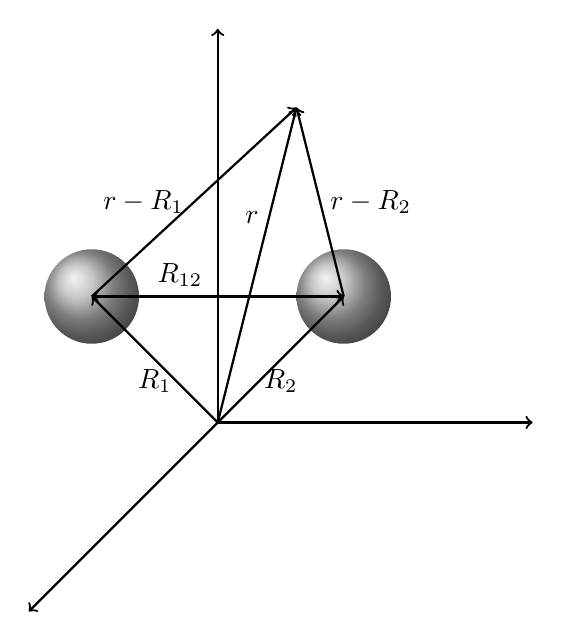
\begin{tikzpicture}[thick,scale=2]
	\draw[<->] (0,2.5)--(0,0)--(2,0);
	\draw[->] (0,0)--(-1.2,-1.2);
	\shade[ball color=black!30] (0.8,0.8)circle (0.3);
	\shade[ball color=black!30] (-0.8,0.8)circle (0.3);
	\draw[<->] (-0.8,0.8)--node[below]{$\bo{R_1}$}(0,0)--node[below]{$\bo{R_2}$}(0.8,0.8);
	\draw[<->](-.8,.8)--node[above,pos=.35]{$\bo{R_{12}}$}(.8,.8);
	\draw[->] (-.8,.8)--node[above,left]{$\bo{r-R_1}$}(.5,2);
	\draw[->] (.8,.8)--node[above,right]{$\bo{r-R_2}$}(.5,2);
	\draw[->] (0,0)--node[above,left,pos=.65]{$\bo{r}$}(.5,2);
	\end{tikzpicture}
	\caption{\phrase{极小基 $\hd$}的坐标}
	\label{f2.5}
\end{figure} 
重叠积分依赖于距离$R_{12}=|\bo{R_1-R_2}|$, 
$R_{12}=0$则$S_{12}=1$, 
$R_{12}=\infty$那么$S_{12}=0$.


利用两个定域原子轨道$\phi_1,\phi_2$, 
可以采取线性组合的方式构建两个离域分子轨道. 
对称组合生成$gerade$宇称的成键分子轨道(所谓gerade对称是指, 
以两核之间的中点作为反演点, 
将分子轨道反演, 
轨道保持不变, 
即对称).
:
\begin{equation}
\label{2.57}
\psi_1=[2(1+S_{12})]^{-1/2}(\phi_1+\phi_2)
\end{equation}
相反地也可以构建反对称组合, 
生成具有$ungerade$对称性的反键分子轨道(也即在中点反演下轨道反对称):
\begin{equation}
\label{2.58}
\psi_2=[2(1-S_{12})]^{-1/2}(\phi_1-\phi_2)
\end{equation}
\exercise{请证明$\psi_1,\psi_2$构成一组正交基.}

以上这个最简单的例子所用的是一个普适的技术: 用已知的空间(sptial)基函数将分子轨道展开: 
\begin{equation}
\label{2.59}
\psi_i(\bo{r})=\sum_{\mu=1}^{K}C_{\mu i}\phi_{\mu}(\bo{r})
\end{equation} 

仅用两个基函数描述H$_2$就是所谓的\emph{极小}基组模型. 
在这个体系中, 
基函数的一个很自然的选择就是两个原子原来的轨道$\phi_1,\phi_2$. 
两个基函数正确的线性组合方式由对称性决定, 
而且不需要解Hartree-Fock方程. 
\autoref{2.57}、\autoref{2.58}中的$\psi_1,\psi_2$就是用$\phi_1,\phi_2$展开的Hartree-Fock空间轨道.


给定两个空间轨道$\psi_1,\psi_2$, 
可以构成四个自旋轨道:
\begin{equation}
\begin{split}
\chi_1(\bo{x})=\psi_1(\bo{r})\alpha(\omega)\\
\chi_2(\bo{x})=\psi_1(\bo{r})\beta(\omega)\\
\chi_3(\bo{x})=\psi_2(\bo{r})\alpha(\omega)\\
\chi_4(\bo{x})=\psi_2(\bo{r})\beta(\omega)
\end{split}
\label{2.60}
\end{equation}
对应自旋轨道的轨道能量可用Hartree-Fock算符得到. 
但是无需计算就可以发现, 
$\chi_1,\chi_2$是简并的, 
而且有更低的能量, 
对应成键态. 
$\chi_3,\chi_4$也是简并的, 
但能量更高, 
对应反键态. 
此模型的Hartree-Fock基态是单行列式:
\begin{equation}
\ket{\Psi_0}=\ket{\chi_1\chi_2}
\end{equation}
如\autoref{fig2.6}所示.

\begin{figure}[h]
	\begin{tikzpicture}[ thick,scale=2.5]
	% 1st four orbitals psi_0 = 
	\node at (0, 0) {$\ket{\Psi_0}=$};
	\draw (0.7,0.2)node[left]{$\chi_3$}--(1.5,0.2);
	\draw (1.7,0.2)--(2.5,0.2)node[right]{$\chi_3$};
	\draw (0.7,-.2)node[left]{$\chi_1$}--(1.5,-.2);
	\draw (1.7,-.2)--(2.5,-.2)node[right]{$\chi_2$};
	\node at(1.1,-.25) {\Huge\bf*};
	\node at(2.1,-.25) {\Huge\bf*};
	\node at (0.2, -1.2){$\equiv$};
	\draw (0.7, -1)node[left]{$\chi_3$}--(1.5, -1);
	\draw (1.7, -1)--(2.5, -1)node[right]{$\chi_4$};
	% replac asterisk by arrow 
	\draw (0.7,-1.4)node[left]{$\chi_1$}--(1.5,-1.4);
	\draw (1.7,-1.4)--(2.5,-1.4)node[right]{$\chi_2$};
	\node at(1.1,-1.4) {$\bm{\big\uparrow}$};
	\node at(2.1,-1.4) {$\bm{\big\downarrow}$};
	
	\node at (0.8,-2.4){$\equiv$};
	\draw (1.2,-2.2)--(2.0,-2.2)node[right]{$\psi_2$};
	\draw (1.2,-2.6)--(2.0,-2.6)node[right]{$\psi_1$};
	\node at(1.47,-2.6) {$\bm{\big\uparrow}$};
	\node at(1.73,-2.6) {$\bm{\big\downarrow}$};
	\end{tikzpicture}
	\caption{H$_2$的Hartree-Fock基态: 3种表达法}
		\label{fig2.6}
\end{figure}
有时用自旋轨道空间部分的记号来标记自旋轨道本身, 
符号上面有无横线代表自旋是$\alpha$或$\beta$:
\begin{equation}
\begin{split}
\chi_1\equiv\psi_1\qquad\qquad\chi_2\equiv\bar{\psi}_1\\
\chi_3\equiv\psi_2\qquad\qquad\chi_4\equiv\bar{\psi}_2
\end{split}
\end{equation}
用这种记号, 
Hartree-Fock基态就写成:
\begin{equation}
\ket{\Psi_0}=\ket{\psi_1\bar{\psi}_1}=\ket{1\bar{1}}
\end{equation}
这种符号代表两个电子占据同一个空间轨道$\psi_1$, 
一个自旋是$\alpha$一个是$\beta$. 
从上下文可以清楚地分辨出$\psi_1$是代表空间轨道还是由$\psi_1$和$\alpha$自旋函数组成的自旋轨道.


\subsection{被激发的(Slater)行列式}
 \label{sec2.2.6}
Hartree-Fock这种手续生成一组$2K$个自旋轨道$\{\chi_i\}$. Hartree-Fock基态:
\begin{equation}
\label{2.64}
\ket{\Psi_0}=\ket{\chi_1\chi_2\cdots\chi_a\chi_b\cdots\chi_N}
\end{equation}
是单行列式形式下, 
对基态的最优近似(以变分的意义来说). 
然而很明显, 
用$2K>N$个自旋轨道可以构建很多行列式, 
Hartree-Fock基态只是其中之一. 
从$2K$个物品中一次性取出$N$个的取法数目为(即二项式系数):
\begin{equation*}
\binom{2K}{N}=\frac{(2K)!}{N!(2K-N)!}
\end{equation*}

这也是2K个自旋轨道能构成的$N$电子单行列式的数目; 
Hartree-Fock基态只是其一. 
我们可以如此表示这些行列式: 将Hartree-Fock基态\autoref{2.64}作为参考态, 
将其他行列式按照它们与参考态的不同来分类, 
也就是: \autoref{2.64}中的某个自旋轨道(或穴)$\{\chi_a\}$替换为了哪个虚轨道(或粒子自旋轨道). 
这些其他的行列式可以认为是体系激发态的一个近似. 
很快我们就可以知道, 
由这些行列式和$\Psi_0$可以给出对体系基态或激发态更精确的描述.


单重激发态是指在Hartree-Fock基态中占据某轨道$\chi_a$的电子被提升到了某虚轨道$\chi_r$上:

\begin{equation}
\ket{\Psi_a^r}=\ket{\chi_1\chi_2\cdots\chi_r\chi_b\cdots\chi_N}
\end{equation}
见\autoref{f2.7}.


双重激发态(见\autoref{f2.8})是$\chi_a,\chi_b$上的电子被激发到$\chi_r,\chi_s$:
\begin{equation}
\ket{\Psi_{ab}^{rs}}=\ket{\chi_1\chi_2\cdots\chi_r\chi_s\cdots\chi_N}
\end{equation}

总共$\binom{2K}{N}$个行列式都可按照Hartree-Fock基态或者单重、二重,
三重、四重……N重激发态来分类. 
某种程度上, 
行列式的重数越高, 
在近似描述体系的真实态时, 
其重要性就越低. 
虽然激发态行列式描述的不是真实的激发态, 
但重要的是, 
它们可以作为$N$电子基函数来展开精确的$N$电子态.

\begin{figure}[H]
	\begin{minipage}[t]{0.3\textwidth}
	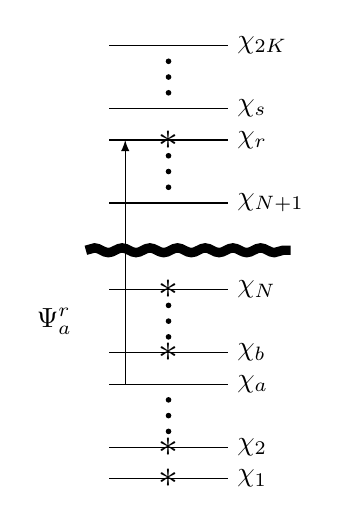
\begin{tikzpicture}[baseline={(0,.2)}]
	\draw[](0,0)--node{\Large$*$}+(1.5,0)node[right]{$\chi_1$};
	\draw[](0,.4)--node{\Large$*$}+(1.5,0)node[right]{$\chi_2$};
	\filldraw (.75,.6)circle(.8pt) (.75,.8)circle(.8pt) (.75,1.0)circle(.8pt);
	\draw  (0,1.2)--node{}+(1.5,0)node[right]{$\chi_a$};
	\draw  (0,1.6)--node{\Large$*$}+(1.5,0)node[right]{$\chi_b$};
	\filldraw (.75,1.8)circle(.8pt) ++(0,.2)circle(.8pt) ++(0,.2)circle(.8pt);
	\draw  (0,2.4)--node{\Large$*$}+(1.5,0)node[right]{$\chi_N$};
	\draw[line width=1.2mm,style={decorate, decoration={snake, amplitude=.3mm}}] (-.3,2.9)--++(2.6,0);
	\draw (0,3.5)--+(1.5,0)node[right]{$\chi_{N+1}$};
	\filldraw (.75,3.7)circle(.8pt) ++(0,.2)circle(.8pt) ++(0,.2)circle(.8pt);
	\draw (0,4.3)--node{\Large$*$}+(1.5,0)node[right]{$\chi_{r}$};
	\draw (0,4.7)--+(1.5,0)node[right]{$\chi_{s}$};
	\filldraw (.75,4.9)circle(.8pt) ++(0,.2)circle(.8pt) ++(0,.2)circle(.8pt);
	\draw (0,5.5)--+(1.5,0)node[right]{$\chi_{2K}$};
	\draw[arrows =-latex] (.2,1.2)--++(0,3.1);
	\draw (-.7,2)node{$\displaystyle\ket{\Psi_a^r}$};
	\end{tikzpicture}\end{minipage}\qquad
	\begin{minipage}[t]{0.6\textwidth}
		\caption{一个单激发行列式.}\label{f2.7}\end{minipage}
\end{figure}
\begin{figure}[H]
	\begin{minipage}[t]{0.3\textwidth}
		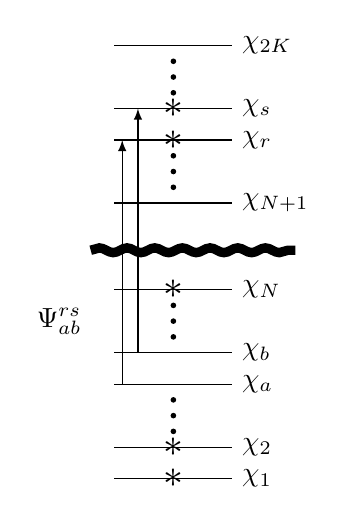
\begin{tikzpicture}[baseline={(0,.2)}]
		\draw[](0,0)--node{\Large$*$}+(1.5,0)node[right]{$\chi_1$};
		\draw[](0,.4)--node{\Large$*$}+(1.5,0)node[right]{$\chi_2$};
		\filldraw (.75,.6)circle(.8pt) (.75,.8)circle(.8pt) (.75,1.0)circle(.8pt);
		\draw  (0,1.2)--node{}+(1.5,0)node[right]{$\chi_a$};
		\draw  (0,1.6)--node{}+(1.5,0)node[right]{$\chi_b$};
		\filldraw (.75,1.8)circle(.8pt) ++(0,.2)circle(.8pt) ++(0,.2)circle(.8pt);
		\draw  (0,2.4)--node{\Large$*$}+(1.5,0)node[right]{$\chi_N$};
		\draw[line width=1.2mm,style={decorate, decoration={snake, amplitude=.3mm}}] (-.3,2.9)--++(2.6,0);
		\draw (0,3.5)--+(1.5,0)node[right]{$\chi_{N+1}$};
		\filldraw (.75,3.7)circle(.8pt) ++(0,.2)circle(.8pt) ++(0,.2)circle(.8pt);
		\draw (0,4.3)--node{\Large$*$}+(1.5,0)node[right]{$\chi_{r}$};
		\draw (0,4.7)--node{\Large$*$}+(1.5,0)node[right]{$\chi_{s}$};
		\filldraw (.75,4.9)circle(.8pt) ++(0,.2)circle(.8pt) ++(0,.2)circle(.8pt);
		\draw (0,5.5)--+(1.5,0)node[right]{$\chi_{2K}$};
		\draw[arrows =-latex] (.1,1.2)--++(0,3.1);
		\draw[arrows =-latex] (.3,1.6)--(.3,4.7);
		\draw (-.7,2)node{$\displaystyle\ket{\Psi_{ab}^{rs}}$};
		
		\end{tikzpicture}\end{minipage}\qquad
	\begin{minipage}[t]{0.6\textwidth}
		\caption{一个双激发行列式.}\label{f2.8}\end{minipage}
\end{figure}


\subsection{从精确波函数到组态相互作用}
 \label{sec2.2.7}
现在来看如何将激发态行列式用作$N$电子基函数. 
想象有一组完全集$\{\chi_i(x)\}$. 
任意单变量函数$\Phi(x_1)$都可以展开成:
\begin{equation}
	\Phi(x_1)=\sum_ia_i\chi_x(x_1)
\end{equation}
$a_i$是展开系数. 那么, 如何展开两个变量的函数$\Phi(x_1,x_2)$? 如果想象$x_2$被固定, 那么可以将$\Phi(x_1,x_2)$展成:
\begin{equation}
\label{2.68}
\Phi(x_1,x_2)=\sum_ia_i(x_2)\chi_i(x_1)
\end{equation}
展开系数现在是$x_2$的函数. 
由于$a_i(x_2)$是单变量的, 
可用完全集$\{\chi_i \}$将其展开:
\begin{equation}
a_i(x_2)=\sum_jb_{ij}\chi_j(x_2)
\end{equation}
代到\autoref{2.68}内得到:
\begin{equation}
\Phi(x_1,x_2)=\sum_i\sum_jb_{ij}\chi_j(x_2)\chi_i(x_i)
\end{equation}
若要求$\Phi$反对称:
\begin{equation}
\Phi(x_1,x_2)=-\Phi(x_2,x_1)
\end{equation}
那么$b_{ij}=-b_{ji},b_{ii}=0$, 
那么
\begin{equation}
\begin{split}
\Phi(x_1,x_2)&=\sum_i\sum_{j>i}b_{ij}[\chi_i(x_1)\chi_j(x_2)-\chi_j(x_1)\chi_i(x_2)]\\
&=\sum_{i<j}2^{1/2}b_{ij}\ket{\chi_i\chi_j}
\end{split}
\end{equation}
可见, 
任意反对称的两变量函数都可以由完全集$\{\chi_i(x)\}$构成的所有(二阶)行列式展开. 
这个结论容易扩展到多变量情形. 
所以, 
$N$电子问题中的基态和激发态精确波函数都可以写成由一组完全集$\{\chi_i(x) \}$所生成的全部可能的$N$电子Slater行列式的线性组合.


由于所有可能的行列式都可以借助基态Hartree-Fock行列式(的激发)来表示, 
所以可将体系任意态对应的精确波函数写作:
\begin{equation}
\ket{\Phi}=c_0\ket{\Psi_0}+\sum_{ra}c_a^r\ket{\Psi_a^r}+\sum_{\substack{a<b\\r<s}}c_{ab}^{rs}\ket{\Psi_{ab}^{rs}}+\sum_{\substack{a<b<c\\r<s<t}}c_{abc}^{rst}\ket{\Psi_{abc}^{rst}}+\cdots
\end{equation}
求和号下的$a<b$是指对所有$a$以及所有大于$a$的$b$求和(即对所有的占据轨道对进行求和). 
同样, 
$r<s$代表对所有虚轨道对进行求和. 
由此, 
展开中就包含了所有双激发组态. 
三重和更高激发行列式的情况是一样的. 
所以, 
无穷集合$\{\ket{\Psi_i} \}=\{\ket{\Psi_0}, \ket{\Psi_a^r}, \ket{\Psi_{ab}^{rs}}, \cdots \}$就是完备集, 
可用于展开$N$电子波函数. 
由完备集$\ket{\Psi_i}$生成的哈密顿算符矩阵, 
其本征值就是基态和激发态的准确能量(哈密顿算符矩阵即矩阵元为$\braket{\Psi_i|\scr{H}|\Psi_j}$的矩阵.
) 由于每个$\ket{\Psi_i}$都对应一种自旋轨道的组态(组态即生成$\ket{\Psi_i}$的那些自旋轨道), 
所以这种方法叫作\emph{组态相互作用configuration interaction ({CI\rm})}. 
CI在第四章有详细阐述. 
哈密顿矩阵的最低本征值, 
记为$\scr{E}_0$, 
就是Born-Oppenheimer近似下体系精确的非相对论基态能量. 
这个能量与Hartree-Fock极限能量$E_0$的差值就叫作\emph{相关能}:
\begin{equation}
E_{\mathrm{corr}}=\scr{E}_0-E_0
\end{equation} 
这个差值不为0是因为Hartree-Fock近似下, 
有相反自旋的电子的运动没有相关.


可惜上面的程序无法实际运用于多电子问题, 
即无法如此求得多电子问题所有的解, 
这是由于我们无法处理无限基组. 
若采用有限个自旋轨道$\{\chi_i|i=1,2,\cdots,2K \}$, 
那么这些轨道构成的$\binom{2K}{N}$个行列式就不是完备的$N$电子基. 
然而, 
若将这些行列式生成的有限维哈密顿矩阵对角化, 
我们就得到这2K个自旋轨道张成的单电子子空间内的精确解(即在这个子空间内是最精确的), 
换一种等价的说法, 
就是这$\binom{2K}{N}$个行列式构成的$N$电子子空间内的精确解. 
这种程序叫\emph{full CI}. 
即使是较小的体系, 
采用极小基, 
full CI所需要的行列式数目仍十分巨大. 
因此在实际操作中, 
需要对full CI展开进行截断, 
即仅用$\binom{2K}{N}$个行列式中的一小部分进行计算. 
\autoref{f2.9}是Born-Oppenheimer近似下的非相对论波函数随单电子和$N$电子基组数目增长的关系.


\exercise{苯的极小基包含72个自旋轨道. 计算由行列式生成的full CI的矩阵的大小. 其中有多少单激发行列式, 多少双激发行列式? }

下面以$\text{H}_2$极小基模型为例, 
阐述以上操作的核心 .

\begin{figure}[H]
	\begin{tikzpicture}
\begin{axis}[
%standard,
%ticks=none,
axis y line=center,
axis x line=middle, 
%axis x line shift=-.55,
every axis x label/.style={at={(axis description cs:.5,-.1)}},
xlabel={Slater行列式的数目$\binom{2K}{N}$},
every axis y label/.style={rotate=90,at={(axis description cs:-0.13,.54)}},
ylabel={空间轨道基函数的数目K},
%	axis on top=true,
xmin=0,
xmax=5.9,
xtick={1,2,3,4,5},
xticklabels={1,10,100,1000,10000},
%x tick label style={
%	/pgf/number format/1000 sep=},
%extra x ticks={2,4,6,8,12,18,14},
%extra x tick style={xticklabel style={yshift=0.5ex, anchor=south}},
ymin=0,
ymax=57,
ytick distance=10,
height=.7\textwidth,
width=.7\textwidth,]
\draw[->, thick] (axis cs: 1,24)--(axis cs: 1,50)node[above]{{极限}};
\draw (axis cs:1,53)node[above]{{Hartree-Fock}};
\draw[->, thick] (axis cs:2.1,33)--(axis cs:4.7,50)node[above]{精确结果};
\draw[->,thick] (axis cs:1.8,27)--(axis cs:4.7,27)node[right]{Full CI};
\end{axis}
\end{tikzpicture}
\caption{单电子基组和N电子基组的大小对计算的影响}\label{f2.9}
\end{figure}
之前提到(\autoref{2.60})该模型有四($2K=4$)个自旋轨道$\chi_1,\chi_2,\chi_3,\chi_4$. 
$N=2$, 
那么可以构造$\dbinom{4}{2}=\dfrac{4!}{2!2!}=6$个不重复的行列式. 
Hartree-Fock基态行列式是:
\begin{equation}
\ket{\Psi_0}=\ket{\chi_1\chi_2}=\ket{\psi_1\bar{\psi}_1}=\ket{1\bar{1}}\qquad
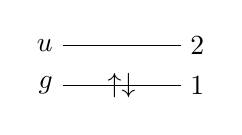
\begin{tikzpicture}[baseline={([yshift=-.8ex]current bounding box.center)}]
\draw (0,0)node[left] {$u$}--(1.5,0)node[right]{2};
\draw (0,-0.5)node[left] {$g$}--node[pos=0.5]{$\uparrow\downarrow$}(1.5,-0.5)node[right]{1};
\end{tikzpicture}
\end{equation}
单激发行列式为:
\begin{subequations}\label{eq:2.76}
    \begin{align}
\ket{\Psi_1^2}=\ket{2\bar{1}}\qquad
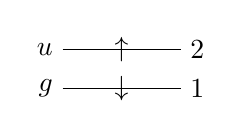
\begin{tikzpicture}[baseline={([yshift=-.8ex]current bounding box.center)}]
\draw (0,0)node[left] {$u$}--node[pos=0.5]{$\uparrow$}(1.5,0)node[right]{2};
\draw (0,-0.5)node[left] {$g$}--node[pos=0.5]{$\downarrow$}(1.5,-0.5)node[right]{1};
\end{tikzpicture}
\\
\ket{\Psi_1^{\bar{2}}}=\ket{\bar{21}}\qquad
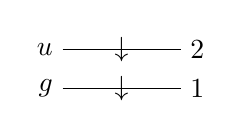
\begin{tikzpicture}[baseline={([yshift=-.8ex]current bounding box.center)}]
\draw (0,0)node[left] {$u$}--node[pos=0.5]{$\downarrow$}(1.5,0)node[right]{2};
\draw (0,-0.5)node[left] {$g$}--node[pos=0.5]{$\downarrow$}(1.5,-0.5)node[right]{1};
\end{tikzpicture}
\\                                                                                                    \ket{\Psi_{\bar{1}}^2}=\ket{{12}}\qquad
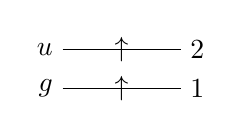
\begin{tikzpicture}[baseline={([yshift=-.8ex]current bounding box.center)}]
\draw (0,0)node[left] {$u$}--node[pos=0.5]{$\uparrow$}(1.5,0)node[right]{2};
\draw (0,-0.5)node[left] {$g$}--node[pos=0.5]{$\uparrow$}(1.5,-0.5)node[right]{1};
\end{tikzpicture}
\\
\ket{\Psi_{\bar{1}}^{\bar{2}}}=\ket{1\bar{2}}\qquad
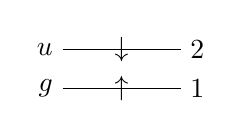
\begin{tikzpicture}[baseline={([yshift=-.8ex]current bounding box.center)}]
\draw (0,0)node[left] {$u$}--node[pos=0.5]{$\downarrow$}(1.5,0)node[right]{2};
\draw (0,-0.5)node[left] {${g}$}--node[pos=0.5]{$\uparrow$}(1.5,-0.5)node[right]{1};
\end{tikzpicture}
    \end{align}
\end{subequations}
双激发行列式只有一个:
\begin{equation}
\ket{\Psi_{1\bar{1}}^{2\bar{2}}}=\ket{2\bar{2}}=\ket{\chi_3\chi_4}=\ket{\Psi_{12}^{34}}\qquad
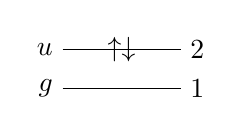
\begin{tikzpicture}[baseline={([yshift=-.8ex]current bounding box.center)}]
\draw (0,0)node[left] {$u$}--node[pos=0.5]{$\uparrow\downarrow$}(1.5,0)node[right]{2};
\draw (0,-0.5)node[left] {$g$}--(1.5,-0.5)node[right]{1};
\end{tikzpicture}
\end{equation}
局限在极小基组张成的空间内, 
精确波函数就是这六个行列式的线性组合. 
Hartree-Fock基态中两个电子都在gerade轨道上, 
所以此态有g对称性(正乘正得正). 
双激发行列式中两个电子在ungerade轨道上, 
此态对称性也为g(负乘负得正). 
剩余的单激发行列式中电子一个在gerade轨道一个在ungerade轨道, 
因此这些态对称性都是u(正乘负得负). 
\phrase{极小基 $\mathrm{H}_2$}的精确波函数$\ket{\Phi_0}$的对称性与Hartree-Fock近似下的基态一样, 
都有$g$对称性. 
因此, 
只有带$g$对称性的行列式会出现在$\ket{\Phi_0}$的展开中, 
即
\begin{equation}
\ket{\Phi_0}=c_0\ket{\Psi_0} + c_{1\bar{1}}^{2\bar{2}}\ket{\Psi_{1\bar{1}}^{2\bar{2}}}=c_0\ket{\Psi_0} + c_{12}^{34}\ket{\Psi_{12}^{34}}
\end{equation}
确定了上述展开式中的系数, 
也就确定了精确波函数$\ket{\Phi_0}$和精确能量$\braket{\Phi_0|\mathscr{H}|\Phi_0}$. 
为此, 
我们需将全组态相互作用(full CI)矩阵对角化, 
也即将以$\ket{\Psi_0}$和$\ket{\Psi_{1\bar{1}}^{2\bar{2}}}$为基底的$2\times 2$哈密顿矩阵对角化:
\begin{equation}
	\label{2.79}
	\mathbf{H}=
	\begin{pmatrix}
		\braket{{\Psi_0}|\mathscr{H} | {\Psi_0}} & \braket{{\Psi_0} |\mathscr{H} |{\Psi_{1\bar{1}}^{2\bar{2}}}}\\
		\braket{{\Psi_{1\bar{1}}^{2\bar{2}}}|\mathscr{H} | {\Psi_0}} & \braket{{\Psi_{1\bar{1}}^{2\bar{2}}} |\mathscr{H} |{\Psi_{1\bar{1}}^{2\bar{2}}}}
	\end{pmatrix}
\end{equation}

问题到此没有结束, 
因为我们还不知道如何求出行列式之间的哈密顿矩阵元, 
这在其他量子化学方法中也是常见的问题. 
我们下节进行介绍.


\section{算符及其矩阵元 }
 \label{sec2.3}
本节来讲如何求得某算符在正交归一轨道构成的行列式之间的矩阵元. 
今有某算子$\mathcal{O}$与两个$N$电子行列式$\ket{K},\ket{L}$, 
如何求得$\braket{K|\mathcal{O}|L}$? 所谓求矩阵元, 
指的是将这个积分化为仅包含自旋轨道$\chi_i$的积分($\chi_i$即$\ket{K},\ket{L}$中的轨道), 
然后再约化为仅包含空间轨道$\psi_i$的积分. 
 我们将以\phrase{极小基 $\mathrm{H}_2$}为例展示该过程, 
然后给出求这种矩阵元的一般规则.


\subsection{\phrase{极小基 $\mathrm{H}_2$}的矩阵元}
 \label{sec2.3.1}
我们先来计算\phrase{极小基 $\mathrm{H}_2$}模型的full CI矩阵元(方程\autoref{2.79}). 
该模型的精确基态是Hartree-Fock基态$\ket{\Phi_0}=\ket{\chi_1\chi_2}=\ket{1\bar{1}}$和双激发态$\ket{\Phi_{12}^{34}}=\ket{\chi_3\chi_4}=\ket{\Phi_{1\bar{1}}^{2\bar{2}}}=\ket{2\bar{2}}$的线性组合, 
我们要做的是求出对角元$\braket{{\Phi_0}|\mathscr{H} | {\Phi_0}}$, 
$\braket{{\Phi_{1\bar{1}}^{2\bar{2}}} |\mathscr{H} |{\Phi_{1\bar{1}}^{2\bar{2}}}}$(即Hartree-Fock基态和双激发态的能量)以及非对角元$\braket{{\Phi_0} |\mathscr{H} |{\Phi_{1\bar{1}}^{2\bar{2}}}},$$\,\braket{{\Phi_{1\bar{1}}^{2\bar{2}}}|\mathscr{H} | {\Phi_0}}$.


双电子体系的哈密顿量为
\begin{align}
\mathscr{H}&=\left( -\frac{1}{2}\nabla_1^2 - \sum_A\frac{Z_A}{r_{1A}} \right) + \left( -\frac{1}{2}\nabla_2^2 - \sum_A\frac{Z_A}{r_{2A}} \right) + \frac{1}{r_{12}}\notag\\
&=h(1) + h(2) + \frac{1}{r_{12}}
\end{align}
其中$h(1)$是电子1的``核哈密顿量", 
代表电子在核的势场中的动能和势能, 
此即``核哈密顿量"的由来. 
为了方便, 
将总哈密顿量分成单电子和双电子部分:
\begin{align}
\mathcal{O}_1&=h(1)+h(2)
\label{2.81}
\end{align}
\begin{align}
\mathcal{O}_2&=r_{12}^{-1}
\end{align}

先来考虑矩阵元$\braket{\Psi_0|\mathcal{O}_1|\Psi_0}$, 
由\autoref{2.81}可知它是两项之和. 
第一项为
\begin{align}
\braket{\Psi_0|h(1)|\Psi_0}=&\int\db{x}_1\db{x}_2\left[2^{-1/2}\left(\chi_1(\mathbf{x}_1)\chi_2(\mathbf{x}_2)-\chi_2(\mathbf{x}_1)\chi_1(\mathbf{x}_2)\right)\right]^*\notag\\
\qquad&\times h(\mathbf{r}_1)\left[ 2^{-1/2}\left(\chi_1(\mathbf{x}_1)\chi_2(\mathbf{x}_2)-\chi_2(\mathbf{x}_1)\chi_1(\mathbf{x}_2)\right)\right]\notag\\
=\frac{1}{2}\int\dd{\mathbf{x}_1}\dd\mathbf{x}_2\{\chi_1^*(\mathbf{x_1})&\chi_2^*(\mathbf{x}_2)h(\mathbf{r}_1)\chi_1(\mathbf{x}_1)\chi_2(\mathbf{x}_2) + \chi_2^*(\mathbf{x}_1)\chi_1^*(\mathbf{x}_2)h(\mathbf{r}_1)\chi_2(\mathbf{x_1})\chi_1(\mathbf{x}_2) \notag\\
 - \chi_1^*(\mathbf{x}_1)&\chi_2^*(\mathbf{x}_2)h(\mathbf{r}_1)\chi_2(\mathbf{x}_1)\chi_1(\mathbf{x}_2) + \chi_2^*(\mathbf{x}_1)\chi_1^*(\mathbf{x}_2)h(\mathbf{r}_1)\chi_1(\mathbf{x_1})\chi_2(\mathbf{x}_2)
\}
\end{align}
上式的四项中, 
对$\mathbf{x}_2$的积分不是1(前两项)就是0(后两项), 
这是由于自旋轨道的正一性. 
因此有
\begin{equation}
\braket{\Psi_0|h(1)|\Psi_0}=\frac{1}{2}\int\dd\mathbf{x}_1\chi_1^*(\mathbf{x}_1)h(\mathbf{r}_1)\chi_1(\mathbf{x}_1)+\frac{1}{2}\int\dd\mathbf{x}_1\chi_2^*(\mathbf{x}_1)h(\mathbf{r}_1)\chi_2(\mathbf{x}_1)
\end{equation}
以同样的手续, 
可以求得$\braket{\Psi_0|h(2)|\Psi_0}=\braket{\Psi_0|h(1)|\Psi_0}$, 
那么
\begin{equation}
\braket{\Psi_0|\mathcal{O}_1|\Psi_0}=\int\dd\mathbf{x}_1\chi_1^*(\mathbf{x}_1)h(\mathbf{r}_1)\chi_1(\mathbf{x}_1) + \int\dd\mathbf{x}_1\chi_2^*(\mathbf{x}_1)h(\mathbf{r}_1)\chi_2(\mathbf{x}_1)
\end{equation}
上式中的积分叫作\emph{单电子积分}, 
也即, 
积分都是对单个电子的坐标作的. 
单电子积分中的积分变量习惯上都选成电子1的坐标. 
我们引入如下记号来表示包含自旋轨道的单电子积分:
\begin{equation}
\braket{i|h|j}=\braket{\chi_i|h|\chi_j}=\int\dd\mathbf{x}_1\chi_i^*(\mathbf{x}_1)h(\mathbf{r}_1)\chi_j(\mathbf{x}_1)
\end{equation}
那么有
\begin{equation}
\braket{\Psi_0|\mathcal{O}|\Psi_0}=\braket{1|h|1}+\braket{2|h|2}
\end{equation}

\exercise{
请证明
\begin{equation*}
\braket{\Psi_{12}^{34}|\mathcal{O}_1|\Psi_{12}^{34}}=\braket{3|h|3}+\braket{4|h|4}
\end{equation*}
以及
\begin{equation*}
\braket{\Psi_{0}|\mathcal{O}_1|\Psi_{12}^{34}}=
\braket{\Psi_{12}^{34}|\mathcal{O}_1|\Psi_0}=0
\end{equation*}
}

现来计算$\mathcal{O}_2$的矩阵元:
\begin{align}
\braket{\Psi_0|\mathcal{O}_2|\Psi_0}=&\int\dd\mathbf{x}_1\dd\mathbf{x}_2[2^{-1/2}(\chi_1(\mathbf{x}_1)\chi_2(\mathbf{x}_2)-\chi_2(\mathbf{x}_1)\chi_1(\mathbf{x}_2))]^*\notag\\
\qquad&\times r_{12}^{-1} [2^{-1/2}(\chi_1(\mathbf{x}_1)\chi_2(\mathbf{x}_2)-\chi_2(\mathbf{x}_1)\chi_1(\mathbf{x}_2))]\notag\\
=&\frac{1}{2}\int\dd{\mathbf{x}_1}\dd{\mathbf{x}_2}\{\chi_1^*(\mathbf{x}_1)\chi_2^*(\mathbf{x}_2)r_{12}^{-1}\chi_1(\mathbf{x}_1)\chi_2(\mathbf{x}_2) + \chi_2^*(\mathbf{x}_1)\chi_1^*(\mathbf{x}_2)r_{12}^{-1}\chi_2(\mathbf{x_1})\chi_1(\mathbf{x}_2) \notag\\
\qquad& - \chi_1^*(\mathbf{x}_1)\chi_2^*(\mathbf{x}_2)r_{12}^{-1}\chi_2(\mathbf{x}_1)\chi_1(\mathbf{x}_2) - \chi_2^*(\mathbf{x}_1)\chi_1^*(\mathbf{x}_2)r_{12}^{-1}\chi_1(\mathbf{x_1})\chi_2(\mathbf{x}_2)
\}
\end{align}
由于$r_{12}=r_{21}$, 
上式第二项中$\chi_1$与$\chi_2$的积分变量可以交换, 
所以该项与第一项相等. 
类似地, 
第三项和第四项也相等. 
因此有
\begin{align}
\braket{\Psi_0|\mathcal{O}_2|\Psi_0}=\int&\dd\mathbf{x}_1\dd\mathbf{x}_2 \chi_1^*(\mathbf{x}_1)\chi_2^*(\mathbf{x}_2)r_{12}^{-1}\chi_1(\mathbf{x}_1)\chi_2(\mathbf{x}_2)\notag\\
 -& \int\dd\mathbf{x}_1\dd\mathbf{x}_2\chi_1^*(\mathbf{x}_1)\chi_2^*(\mathbf{x}_2)r_{12}^{-1}\chi_2(\mathbf{x}_1)\chi_1(\mathbf{x}_2)
\end{align}
上面的积分就是\emph{双电子积分}之一例,
之所以叫双电子,
是因为积分变量包括电子1和2的空间坐标以及两个自旋坐标,
共八个变量。
习惯上,
常将所有双电子积分中的积分变量都写成电子1和2的坐标。
现引入记号来表示含自旋轨道的双电子积分:
\begin{equation}
\braket{ij|kl}=\braket{\chi_i\chi_j|\chi_k\chi_l}=\int\dd\mathbf{x}_1\dd\mathbf{x}_2\chi_i^*(\mathbf{x}_1)\chi_j^*(\mathbf{x}_1)r_{12}^{-1}\chi_k(\mathbf{x}_1)\chi_l(\mathbf{x}_2)
\label{2.90}
\end{equation}
那么就有
\begin{equation}
\braket{\Psi_0|\mathcal{O}|\Psi_0}=\braket{12|12}-\braket{12|21}
\end{equation}
Hartree-Fock基态能量就成为
\begin{align}
\label{2.92}
\braket{\Psi_0|\mathscr{H}|\Psi_0}&=\braket{\Psi_0|\mathcal{O}_1+\mathcal{O}_2|\Psi_0}\notag\\
&=\braket{1|h|1}+\braket{2|h|2}+\braket{12|12}-\braket{12|21}
\end{align}

\exercise{
用刚才介绍的方式写出极小基$\rm H_2$的full CI矩阵:
\begin{equation*}
\mathscr{H}=\begin{pmatrix}
\braket{1|h|1}+\braket{2|h|2} +\braket{12|12}-\braket{12|21} &\braket{12|34}-\braket{12|43}\\

\braket{34|12}-\braket{34|21}& 
\braket{3|h|3}+\braket{4|h|4} +\braket{34|34}-\braket{34|43}

\end{pmatrix}
\end{equation*}
并证明其厄密性.

}

\subsection{单、双电子积分的记法}
\label{sec2.3.2}
在推广上面的结果以及给出$N$电子行列式的矩阵元之前,
先来总结一下此书中所用的几种不同的单、双电子积分的记号。

关于自旋轨道的双电子积分已在\autoref{2.90}中提过,
即:
\begin{equation}
\braket{ij|kl}=\braket{\chi_i\chi_j|\chi_k\chi_l}=\int\dd\mathbf{x}_1\dd\mathbf{x}_2\chi_i^*(\mathbf{x}_1)\chi_j^*(\mathbf{x}_2)r_{12}^{-1}\chi_k(\mathbf{x}_1)\chi_l(\mathbf{x}_2)
\end{equation}
这种记法常叫作物理学家的记号。
注意自旋轨道的复共轭并排出现在积分的左边,
并且电子1的空间自旋坐标先出现。
从以上定义可以知道:
\begin{equation}
\braket{ij|kl}=\braket{ji|lk}
\end{equation}
以及
\begin{equation}
\braket{ij|kl}=\braket{kl|ij}^*
\end{equation}
由于双电子积分经常以如下的组合形式出现,
在此引入一个特别的记号来表示\emph{反对称}双电子积分:
\begin{align}
\braket{ij||kl}&=\braket{ij|kl} - \braket{ij|lk}\notag\\
&=\int\dd\bo{x}_1\dd\bo{x}_2\chi_i^*(\bo{x}_1)\chi_j^*(\bo{x}_2)r_{12}^{-1}(1-\mathscr{P}_{12})\chi_k(\bo{x}_1)\chi_l(\bo{x}_2)
\end{align}
其中$\mathscr{P}_{12}$是一个算子,
它的效果是交换电子1和2的坐标。
注意
\begin{align}
\braket{ij||kk}=0
\label{2.97}
\end{align}

但略有遗憾的是,
还存在另一套自旋轨道双电子积分的记号,
而且还被广泛使用,
尤其是在关于Hartree-Fock理论的文献中。
这套记号常称作化学家的记号,
写作:
\begin{equation}
[ij|kl]=\int\ddx_1\ddx_2\chi_i^*(\bo{x}_1)\chi_j(\bo{x}_1)r_{12}^{-1}\chi_k^*(\bo{x}_2)\chi_l(\bo{x}_2)
\end{equation}
可以看到在这个记法中,
电子1坐标对应的两个自旋轨道并排出现在左边,
并且复共轭的函数排在第一个。
交换积分变量,
可以得到:
\begin{equation}
[ij|kl]=[kl|ij]\tag{2.99a}
\end{equation}
此外,
若自旋轨道都是实函数,
这正是大多数分子的Hartree-Fock计算中的情况,
就有如下等式:
\begin{align}
[ij|kl]=[ji|kl]=[ij|lk]=[ji|lk]\tag{2.99b}
\end{align}
\addtocounter{equation}{1}
\begin{table}[h]
	\renewcommand\arraystretch{1.5}
	\centering
	\caption{\bf 关于自旋轨道($\chi$)以及关于空间轨道$\psi$的单、双电子积分}
	\begin{tabular}{l}
		\hline
		\multicolumn{1}{c}{\textit{自旋轨道}}\\
		\parbox{\textwidth}{$[i|h|j]=\braket{i|h|j}=\int\ddx_1\chi_i^*(\bo{x}_1)h(\bo{r}_1)\chi_j(\bo{x}_1) $}\\
		$\braket{ij|kl}=\braket{\chi_i\chi_j|\chi_k\chi_l}=\int\ddx_1\ddx_2\chi_i^*(\bo{x}_1)\chi_j^*(\bo{x}_2)r_{12}^{-1}\chi_k(\bo{x}_1)\chi_l(\bo{x}_2)=[ik|jl] $\\
		$[ij|kl]=[\chi_i\chi_j|\chi_k\chi_l]=\int\ddx_1\ddx_2 \chi_i^*(\bo{x}_1)\chi_j(\bo{x}_1)r_{12}^{-1}\chi_k^*(\bo{x}_2)\chi_l(\bo{x}_2) = \braket{ik|jl}$\\
		$\braket{ij||kl}=\braket{ij|kl} - \braket{ij|lk}=\int\ddx_1\ddx_2 \chi_i^*(\bo{x}_1)\chi_j^*(\bo{x}_2)r_{12}^{-1}(1-\mathscr{P}_{12})\chi_k(\bo{x}_1)\chi_l(\bo{x}_2) $\\
		\multicolumn{1}{c}{\textit{空间轨道}}\\
		$(i|h|j)=h_{ij} = (\psi_i|h|\psi_j)=\int\dd\bo{r}_1\psi_i^*(\bo{r}_1)h(\bo{r}_1)\psi_j(\bo{r}_1)$\\
		$(ij|kl)=(\psi_i\psi_j|\psi_k\psi_l)=\int\dd\bo{r}_1\dd\bo{r}_2\psi_i^*(\bo{r}_1)\psi_j(\bo{r}_1)r_{12}^{-1}\psi_k^*(\bo{r_2})\psi_l(\bo{r}_2) $\\
		$J_{ij}\,\,=(ii|jj)$ 库伦积分\\
		$K_{ij}=(ij|ji)$ 交换积分\\\hline
	\end{tabular}
	\label{t2.2}
\end{table}

对关于自旋轨道的单电子积分来说,
化学家和物理学家的记号完全一样:
\begin{align}
[i|h|j]=\braket{i|h|j}=\int\ddx_1\chi_i^*(\bo{x}_1)h(\bo{r}_1)\chi_j(\bo{x}_1)
\end{align}
\autoref{t2.2}总结了本书所涉及的所有单、双电子积分。
以后在考察如何将自旋轨道的积分转化为空间轨道的积分时,
会介绍一种新的符号来表示对空间轨道的积分,
为完整计,
上表也包含了这些记号。



\subsection{矩阵元的一般规则}
\label{sec2.3.3}
我们已经看到,
求两电子Slater行列式之间的矩阵元非常简单。
$N$电子行列式比这要复杂。
现在我们介绍一套系统地推求矩阵元的规则,
其推导留在下一节再说,
如果读者愿意,
跳过推导也没问题。


量子化学中有两类算符。
第一类是单电子算符之和
\begin{align}
\mathcal{O}_1=\sum_{i=1}^N h(i)
\end{align}
其中$h(i)$是仅关于第$i$个电子的算符,
这种算符代表仅依赖于本电子的位置或动量的动力学变量,
而不依赖于其他电子的位置或动量。
比如动能算符,
电子与核吸引之间势的算符,
偶极矩算符等等。
第二类算符是两电子算符之和:
\begin{align}
\label{2.102}
\mathcal{O}_2 = \sum_{i=1}^{N}\sum_{j>i}^N v(i,j)=\sum_{i<j}v(i,j)
\end{align}
其中$v(i,j)$同时依赖于$i$电子和$j$电子的位置(或动量)。
\autoref{2.102}中的求和遍及所有不同的电子对。
两电子间的库伦势为:
\begin{align}
v(i,j)=r_{ij}^{-1}
\end{align}
这是一个两电子算符。


求$\ket{K}$与$\ket{L}$之间的矩阵元$\braket{K|\mathcal{O}|L}$的规则视$\mathcal{O}$为单电子算符($\mathcal{O}_1$)之和还是双电子算符($\mathcal{O}_2$)之和而不同。
此外,
$\braket{K|\mathcal{O}|L}$的值还视$\ket{K}$和$\ket{L}$的差异程度而不同。
我们分三种情况来说:首先,
若两个行列式完全相同,
即矩阵元是一对角元$\braket{K|\mathcal{O}|K}$,
此时将行列式记作
\begin{align}
\ket{K}=\ket{\cdots\chi_m\chi_n\cdots}
\end{align}
第二,
两个行列式只差一个自旋轨道,
$\ket{K}$中的$\chi_m$在$\ket{L}$中变成$\chi_p$,
其余都一样:
\begin{align}
\ket{K}=\ket{\cdots\chi_p\chi_n\cdots}
\end{align}
第三,
两个行列式中有两个自旋轨道不同,

$\ket{K}$中的$\chi_m,\chi_n$在$\ket{L}$中变成$\chi_p,\chi_q$,其余都一样:
\begin{align}
\ket{K}=\ket{\cdots\chi_p\chi_q\cdots}
\end{align}
此时矩阵元为0,
不同的自旋轨道超过三个以上,
矩阵元同样也是0.


\begin{table}[h]
	\renewcommand\arraystretch{1.7}
	\centering
	\caption{\bf 单电子算符在行列式间的矩阵元(关于自旋轨道)}
	\label{t2.3}
	\begin{tabularx}{\textwidth}{lY}
		\hline
		\multicolumn{2}{c}{$\mathcal{O}_1=\sum_{i=1}^Nh(i)$} \\\hline
		Case 1: $\ket{K}=\ket{\cdots mn\cdot}$&\\
		\multicolumn{2}{c}{$\braket{K|\mathcal{O}_1|K} = \sum_m^N [m|h|m]=\sum_m^N\braket{m|h|m}$}\\
		Case 2: \parbox[t]{.5\textwidth}{
		$\ket{K}=\ket{\cdots mn\cdot}$\\
		$\ket{L}\,=\ket{\cdots pn\cdot}$
			}&	\\
		\multicolumn{2}{c}{$\braket{K|\mathcal{O}_1|L} = [m|h|p]=\braket{m|h|p}$}\\
		Case 3: \parbox[t]{5cm}{
			$\ket{K}=\ket{\cdots mn\cdot}$\\
			$\ket{L}\,=\ket{\cdots pq\cdot}$}& \\
		\multicolumn{2}{c}{$\braket{K|\mathcal{O}_1|L} = 0$}\\\hline
		
	\end{tabularx}
\end{table}

\begin{table}[h]
	\renewcommand\arraystretch{1.7}
	\centering
	\caption{\bf 双电子算符在行列式间的矩阵元(关于自旋轨道)}
	\label{t2.4}
	\begin{tabularx}{\textwidth}{lY}
		\hline
		\multicolumn{2}{c}{$\mathcal{O}_2=\sum_{i=1}^N\sum_{j>i}^{N}r_{ij}^{-1} $}\\\hline
		Case 1: $\ket{K}=\ket{\cdots mn\cdot}$&\\
		\multicolumn{2}{c}{$\braket{K|\mathcal{O}_2|K} = \frac{1}{2}\sum_m^N\sum_n^N [mm|nn]-[mn|nm]=\frac{1}{2}\sum_m^N\sum_n^N\braket{mn||mn}$}\\
		Case 2: \parbox[t]{5cm}{
			$\ket{K}=\ket{\cdots mn\cdot}$\\
			$\ket{L}\,=\ket{\cdots pn\cdot}$
		}	&\\
		\multicolumn{2}{c}{$\braket{K|\mathcal{O}_2|L} = \sum_n^N[mp|nn]-[mn|np]=\sum_n^N\braket{mn||pn}$}\\
		Case 3: \parbox[t]{5cm}{
			$\ket{K}=\ket{\cdots mn\cdot}$\\
			$\ket{L}\,=\ket{\cdots pq\cdot}$}&\\
		\multicolumn{2}{c}{$\braket{K|\mathcal{O}_2|L} = [mp|nq]-[mq|np]=\braket{mn||pq}$}\\\hline
	\end{tabularx}
\end{table}

\autoref{t2.3}、\autoref{t2.4}总结了这三种情况下的规则。
注意,
两个行列式的差异越大,
矩阵元的形式就越简单,
即其中的项数越少。
单电子矩阵元在两个行列式相差两个及以上的自旋轨道时为0, 
双电子矩阵元在行列式相差三个及以上自旋轨道时为0。
在表中,
$m,n$为$\ket{K}$中的占据自旋轨道,
对$m$求和就代表对行列式中共N个(占据)自旋轨道求和。


为更好的应用这些规则,
首先两个行列式必须写成有最大相似度的形式。
举个例子,
比如要求$\ket{\Psi_1},\ket{\Psi_2}$之间的某算符的矩阵元
\begin{align}
\ket{\Psi_1}=\ket{abcd}\notag\\
\ket{\Psi_2}=\ket{crds}\notag
\end{align}
乍一看这两个行列式的四列好像完全不同,
但若交换$\ket{\Psi_2}$中的某些列并注意变号,
就得到:
\begin{equation*}
\ket{\Psi_2}=\ket{crds}=-\ket{crsd}=\ket{srcd}
\end{equation*}
现在两个行列式的相似度最大,
只在两列上不一样。
于是可以使用{\textit{情况三}}的规则,
注意到如下对应:
\[\begin{array}{cc}
\ket{K}=\ket{\Psi_1}&\ket{L}=\ket{\Psi_2}\\
m\equiv a & p\equiv s\\
n\equiv b &q\equiv r
\end{array}\]
因此有$\braket{\Psi_1|\mathcal{O}_1|\Psi_2}=0$以及$\braket{\Psi_1|\mathcal{O}_2|\Psi_2}=\braket{ab||sr}$.


通过\autoref{t2.3}\autoref{t2.4}可以快速写出单个行列式$\ket{K}$的能量:
\begin{align}
\label{2.107}
\braket{K|\mathscr{H}|K}=\braket{K|\mathcal{O}_1+\mathcal{O}_2|K}=\sum_m^N\braket{m|h|m}+\frac{1}{2}\sum_m^N\sum_n^N\braket{mn||mn}
\end{align}
其中
\begin{align}
\label{2.108}
h(i)=-\frac{1}{2}\nabla_i^2-\sum_A\frac{Z_A}{r_{iA}}
\end{align}
\autoref{2.107}中的求和是对$\ket{K}$中的占据自旋轨道进行的. 由于(见\autoref{2.97})
\begin{subequations}
\begin{align}
\braket{mm||mm}=\braket{nn||nn}=0
\end{align}
以及
\begin{align}
\braket{mn||mn}=\braket{nm||nm}
\end{align}
\end{subequations}
\autoref{2.107}可以写成:
\begin{align}
\label{2.110}
\braket{K|\mathscr{H}|K}=&\sum_m^N\braket{m|h|m}+\sum_m^N\sum_{n>m}^N\braket{mn||mn}\notag\\
=&\sum_m[m|h|m]+\sum_m^N\sum_{n>m}^N[mm|nn]-[mn|nm]
\end{align}
反对称双电子积分的求和遍及$\ket{K}$中所有不同的占据自旋轨道对$\chi_m,\chi_n$. 
这个事实可以帮我们记忆如何把单个行列式对应的能量用关于自旋轨道的单、双电子积分表示出来:
\textit{
每个占据的自旋轨道$\chi_i$各在总能中贡献一个$\braket{i|h|i}$项,
并且每一对占据自旋轨道$\chi_i,\chi_j$都贡献一个$\braket{ij||ij}$项
}。
因此,
可将$N$电子体系的总能(在单Slater行列式描述下)视作``单电子能量"(即在$\chi_i$轨道上电子所对应的$\braket{i|h|i}$)之和,
再加上每对电子之间的``相互作用能"($\chi_i,\chi_j$上的电子对应着$\braket{ij||ij}$)之和。
在使用这种语言的时候, 
要记住这仅是为方便记忆. 
物理上, 
两电子间的相互作用通过库伦项来体现,
而非反对称的双电子积分.


\exercise{
从\autoref{2.107}推出\autoref{2.110}
\Next
若$\ket{K}=\ket{\chi_1\chi_2\chi_3}$, 
证明
	$$\braket{K|\hs|K}=\braket{1|h|1}+\braket{2|h|2}+\braket{3|h|3}+\braket{12||12}+\braket{13||13} + \braket{23||23}$$}

本书中常要用到Hartree-Fock基态的矩阵元. 
为方便计, 
我们将\autoref{t2.3}和\autoref{t2.4}中的规则重写了一遍, 
并将$a,b$等同于$m,n$(占据轨道), 
$r,s$等同于$p,q$(未占轨道). 
\autoref{t2.5}和\autoref{t2.6}列出了Hartree-Fock基态的矩阵元(\textit{情形1})以及其与单激发行列式的矩阵元(\textit{情形2}), 
以及与双激发行列式的矩阵元(\textit{情形3}).

\begin{table}[h]
	\renewcommand\arraystretch{1.7}
	\centering
	\caption{\bf Hartree-Fock基态下单电子算符的矩阵元}
	\label{t2.5}
	\begin{tabularx}{\textwidth}{lY}
		\hline
		\multicolumn{2}{c}{$\mathcal{O}_1=\sum_{i=1}^Nh(i) $}\\\hline
		Case 1: & $\braket{\Psi_0|\mathcal{O}_1|\Psi_0} = \sum_m^N [a|h|a]=\sum_m^N\braket{a|h|a}$\\
		Case 2: & $\braket{\Psi_0|\mathcal{O}_1|\Psi_a^r} = [a|h|r]=\braket{a|h|r}$\\
		Case 3: & $\braket{\Psi_0|\mathcal{O}_1|\Psi_{ab}^{rs}} = 0$\\\hline
	\end{tabularx}
\end{table}

\begin{table}[h]
	\renewcommand\arraystretch{1.7}
	\centering
	\caption{\bf Hartree-Fock基态下双电子算符的矩阵元}
	\label{t2.6}
	\begin{tabularx}{\textwidth}{lY}
		\hline
		\multicolumn{2}{c}{\parbox{\textwidth}{\centering$\mathcal{O}_2=\sum_{i=1}^N\sum_{j>i}^{N}r_{ij}^{-1} $}}\\\hline
		Case 1: & $\braket{\Psi_0|\mathcal{O}_2|\Psi_0} = \frac{1}{2}\sum_m^N\sum_n^N [aa|bb]-[ab|ba]=\frac{1}{2}\sum_m^N\sum_n^N\braket{ab||ab}$\\
		Case 2: & $\braket{\Psi_0|\mathcal{O}_2|\Psi_a^r} = \sum_n^N[ar|bb]-[ab|br]=\sum_n^N\braket{ab||rb}$\\
		Case 3: & $\braket{\Psi_0|\mathcal{O}_2|\Psi_{ab}^{rs}} = [ar|bs]-[as|br]=\braket{ab||rs}$\\\hline
	\end{tabularx}
\end{table}

利用这些表, 
可以很快写出Hartree-Fock基态的能量(以化学家的记号):
\begin{equation}\label{eq:2.111}
E_0 = \braket{\Phi_0|\hs|\Phi_0} = \sum_{a}^{N}[a|h|a] + \frac{1}{2}\sum_{a}^{N}\sum_{b}^{N}[aa|bb]-[ab|ba]
\end{equation}  
或以物理学家记号:
\begin{equation}
\label{2.112}
E_0 = \sum_{a}^{N}\braket{a|h|a} + \frac{1}{2}\sum_{a}^{N}\sum_{b}^{N}\braket{ab||ab}
\end{equation}
如前所述, 
\autoref{2.112}可以重写成:
\begin{equation}
\label{2.113}
E_0 = \sum_{a}^{N}\braket{a|h|a} + \sum_{a}^{N}\sum_{b>a}^{N}\braket{ab||ab}
\end{equation}
在$\mathrm{H}_2$极小基下, 
$\ket{\Phi_0}=\ket{\chi_1\chi_2}$, 
那么由\autoref{2.113}可得
\begin{align}
E_0 =& \braket{1|h|1} + \braket{2|h|2} + \braket{12||12}\notag\\
    =& \braket{1|h|1} + \braket{2|h|2} + \braket{12|12} - \braket{12|21}
\end{align}
这与之前的结果\autoref{2.92}相同.


\exercise{用上面总结的规则计算$\mathrm{H}_2$极小基下的Full CI矩阵元. 与\autoref{ex:2.9}的结果作比较.
\Next	
证明
\begin{align*}
 & \braket{\Phi_a^r|\mathcal{O}_1|\Phi_b^s}\\
=& 0                                                  & \text{若}a\neq b,r\neq s\\
=& \braket{r|h|s}                                     & \text{若}a  =  b,r\neq s\\
=&-\braket{b|h|a}                                     & \text{若}a\neq b,r=s    \\
=&\sum_c^N\braket{c|h|c}-\braket{a|h|a}+\braket{r|h|r} & \text{若}a=b,r=s
\end{align*}
\Next
$N$电子体系的Hartree-Fock基态能为$^NE_0=\braket{^N\Phi_0|\hs|^N\Phi_0}$. 考虑一个被电离的体系(即其中一个电子被挪出了$\chi_a$轨道),其能量为$^{N-1}E_a=\braket{^{N-1}\Phi_a|\hs|^{N-1}\Phi_a}$, 其中$\ket{^{N-1}\Phi_a}$是除了$\chi_a$之外的被占轨道组成的单Slater行列式.
\[
\ket{^{N-1}\Phi_a} = \ket{\chi_1\chi_2\cdots\chi_{a-1}\chi_{a+1}\cdots\chi_N}
\]
请利用表中的规则, 
证明这个电离过程所需能量为
\begin{equation*}
^NE_0-^{N-1}E_a = \braket{a|h|a} + \sum_b^N \braket{ab||ab}
\end{equation*}
为显出本节介绍的记忆方法的优势, 
在此我们不借助运算来推导以上结果. 
考虑\autoref{fig2.4}中$\ket{^N\Psi_0}$的表示.
若从$\chi_a$中挪去一个电子, 
则需从总能$^NE_0$中要扣除一项\emph{单电子能量}$\braket{a|h|a}$. 
此外, 
之前在$\chi_a$上的电子会与其余电子有相互作用, 
该电子挪走之后,
这些相互作用(即$\sum_{b\neq a}^{N}\braket{ab||ab}$)也要被扣除. 
考虑到$\braket{aa|aa}=0$, 
可以立马得到上面的结果。 

}

\subsection{矩阵元规则的推导}
\label{sec2.3.4}
本节推导\autoref{t2.3}和\autoref{t2.4}中的矩阵元计算规则,
也就是单、双电子算符夹在正交归一自旋轨道构成的$N$电子行列式间的计算规则. 
由自旋轨道$\chi_i(\mathbf{x}_1),\chi_j(\mathbf{x}_1),\cdots,\chi_k(\mathbf{x}_N)$构成的$N$电子Slater行列式的定义是(见\autoref{eq:1.38})):
\begin{equation}\label{eq:2.115}
\ket{\chi_i\chi_k\cdots\chi_k}=(N!)^{-1/2}\sum_{n=1}^{N!}(-1)^{p_n}\mathscr{P}_n\left\{\chi_i(1)\chi_j(2)\cdots\chi_k(N) \right\}
\end{equation}
其中$\chi(\mathbf{x}_l) \equiv \chi(l)$. 
$\mathscr{P}_n$是对电子标号$1,2,\cdots,N$进行$n$阶置换的算符,%“nth”是否宜于译作“n阶”?第n个似更好。
$p_n$是完成该置换所需的置换数(简单交换的数目).

\exercise{
将\autoref{ex:2.14}的结果推广到$N$电子行列式上: 
已知,由自旋轨道组成的Slater行列式$\ket{\chi_i\chi_j\cdots\chi_k}$是单电子算符$h$(见\autoref{2.29})的本征函数, 
请证明它也是单电子哈密顿$\mathscr{H}=\sum_{i=1}^{N}h(i)$(见\autoref{2.28})的本征函数, 
对应本征值为$\epsilon_i+\epsilon_j+\cdots+\epsilon_k$. 
\textit{提示}:由于$\mathscr{H}$在对电子指标的置换操作下是不变的, 
所以它与$\mathscr{P}$对易.

}

现在要计算形如$\braket{K|\mathcal{O}|L}$的矩阵元, 
其中
\begin{equation}
\ket{K} = \ket{\chi_m(1)\chi_n(2)\cdots}
\end{equation}
是由自旋轨道$\chi_m,\chi_n,\cdots$构成的行列式. 
而$\ket{L}$以某种已知的方式不同于$\ket{K}$. 
在考察单、双电子算符\autoref{t2.3}和\autoref{t2.4}中的和\textit{情形}1、2、3之前, 
先令$\mathcal{O}$为单位算符, 
看看由同一套自旋轨道生成的$\ket{K}$和$\ket{L}$之间的重叠$\braket{K|L}$, 
$\ket{L}$如下
\begin{equation}
\ket{L} = \ket{\chi_m'(1)\chi_n'(2)\cdots}
\end{equation}
假设两个行列式已经按最大相似方式进行了排列. 
利用行列式表达\autoref{eq:2.115}, 
我们有
\begin{align}
\braket{K|L} =& (N!)^{-1} \sum_{i}^{N!}\sum_{j}^{N!} (-1)^{p_i}(-1)^{p_j}\int\ddx_1\ddx_2\cdots\ddx_N \notag\\
              &\times \mathscr{P}_i\{\chi_m^*(1)\chi_n^*(2)\cdots\} \mathscr{P}_j\{\chi_m'(1)\chi_n'(2)\cdots\}
\end{align}
设这套自旋轨道正交归一.
若上面的重叠积分非零, 
带撇的自旋轨道就必须与不带撇的自旋轨道对应相等. 
否则就总会有个$0$因子(因为某个$\ket{L}$中的自旋轨道$\chi_n'$与$\ket{K}$中的自旋轨道$\chi_m,\chi_n,\cdots$正交). 
所以, 
若某行列式中的自旋轨道与$\ket{K}$中的不完全相同, 
那么$\ket{K}$就与其正交. 
如过两个行列式中的自旋轨道一致、排列也完美地相同, 
或者说它们是同一个行列式,
那么
\begin{align}
\braket{K|K} =& (N!)^{-1} \sum_{i}^{N!}\sum_{j}^{N!} (-1)^{p_i}(-1)^{p_j}\int\ddx_1\ddx_2\cdots\ddx_N \notag\\
&\times \mathscr{P}_i\{\chi_m^*(1)\chi_n^*(2)\cdots\} \mathscr{P}_j\{\chi_m(1)\chi_n(2)\cdots\}
\end{align}
在上面的求和中, 
仅当在$i$置换中的电子与在$j$置换中的电子都占据相同的自旋轨道时, 积分才不为$0$. 
那么求和中有效的项中, 
两个置换必须相同($i=j$), 
并且$(-1)^{2p_i}=1$, 
所以有
\begin{equation}
\braket{K|K} = (N!)^{-1} \sum_{i}^{N!}\int\ddx_1\ddx_2\cdots\ddx_N\mathscr{P}_i\{\chi_m^*(1)\chi_n^*(2)\cdots\} \mathscr{P}_j\{\chi_m(1)\chi_n(2)\cdots\}
\end{equation}
求和中的每一项都是$1$, 
所以
\begin{equation}
\braket{K|K} = (N!)^{-1}\sum_{i}^{N!}1 = 1
\end{equation}
这就是说, 
$\ket{K}$是归一化的. 
因此我们有
\begin{equation}
\begin{array}{cc}
\braket{K|K} = 1 & \textit{情形1} \\
\braket{K|L} = 0 & \textit{情形2}
\end{array}
\end{equation}

接下来考察单电子算符之和的矩阵元:
\begin{equation}\label{eq:2.123}
\braket{K|\mathcal{O}_1|L} = \braket{K|h(1)+h(2)+\cdots+h(N)|L}
\end{equation}
由于行列式中的电子不可分辨, 
$h(1)$的矩阵元和$h(2),h(3)$等等的矩阵元相同. 
那么\autoref{eq:2.123}中的每一项都相等, 
也就是
\begin{equation}
\braket{K|\mathcal{O}_1|L} = N\braket{K|h(1)|L}
\end{equation}
该式中我们按照惯例选择了电子1的算符. 
先看\textit{情形1}下的结果:
\begin{align}\label{eq:2.125}
\braket{K|\mathcal{O}_1|K} = & N \braket{K|h(1)|L}\notag \\
                           = & N(N!)^{-1}\sum_{i}^{N!}\sum_{j}^{N!} (-1)^{p_i}(-1)^{p_j}\int\ddx_1\ddx_2\cdots\ddx_N \notag\\
                           &\times \mathscr{P}_i\{\chi_m^*(1)\chi_n^*(2)\cdots\}h(1) \mathscr{P}_j\{\chi_m'(1)\chi_n'(2)\cdots\}
\end{align}
在对电子$2,3,\cdots,N$的座标积分时, 
除非所有电子在第$i$个置换和第$j$个置换中占据的轨道完全对应相同,
否则积分就为$0$(自旋轨道的正交性). 
如果电子$2,3,\cdots,N$在两个置换中都占据完全相同的自轨旋道, 
那么电子1在两个置换中所占据的自旋轨道肯定也相同. 
结果就是, 
只有两个置换等同时($i=j$)所得积分才不为$0$.

\begin{align}\label{eq:2.126}
\braket{K|\mathcal{O}_1|K}= & [(N-1)!]^{-1}\sum_{i}^{N!}\int\ddx_1\ddx_2\cdots\ddx_N \notag\\
&\times \mathscr{P}_i\{\chi_m^*(1)\chi_n^*(2)\cdots\}h(1) \mathscr{P}_j\{\chi_m(1)\chi_n(2)\cdots\}
\end{align}
上式对$N!$个置换求和, 
电子1会占据每个自旋轨道$\{\chi_m|m=1,2,\cdots,N\}$各$(N-1)!$次; 
或者换个说法, 
若电子1在某特定的自旋轨道$\chi_m$上, 
则剩余的电子$2,3\cdots,N$在剩余的$(N-1)$个自旋轨道中共有$(N-1)!$种排列方式. 
对电子$2,3\cdots,N$积分仅会产生一个因子$1$(自旋轨道已归一化), 
因此
\begin{align}
\braket{K|\mathcal{O}_1|K}= & (N-1)![(N-1)!]^{-1}\sum_{m}^{N}\int\ddx_1\,\chi_m^*(1)h(1)\chi_m(1) \notag\\
=&\sum_{m}^{N}\braket{m|h|m}\qquad\textit{情形1}
\end{align}
现在来看\textit{情形2}, 
此时两个行列式的差异仅在一个自旋轨道上, 
$\chi_p$出现在$\ket{L}$中而$\ket{K}$中则是$\chi_m$,

\begin{align}
\ket{K} &= \ket{\chi_m(1)\chi_n(2)\cdots}\\
\ket{L} &= \ket{\chi_p(1)\chi_n(2)\cdots}
\end{align}
与在\textit{情形1}中从\autoref{eq:2.125}导出\autoref{eq:2.126}时相同, 
若积分结果不为0, 
则算符的两边必须有相同的置换, 

\begin{align}
\braket{K|\mathcal{O}_1|L}= & [(N-1)!]^{-1}\sum_{i}^{N!}\int\ddx_1\ddx_2\cdots\ddx_N \notag\\
&\times \mathscr{P}_i\{\chi_m^*(1)\chi_n^*(2)\cdots\}h(1) \mathscr{P}_j\{\chi_p(1)\chi_n(2)\cdots\}
\end{align}
由于前面那个置换中轨道$\chi_m$与后一个置换中的任一自旋轨道都正交, 
只有它被电子1占据时, 
才有可能和$h(1)$``联动", 
以使积分不为0. 
固定了电子1之后, 
电子$2,3,\cdots,N$在余下的$N-1$个自旋轨道($\chi_n,\cdots$)中共有$(N-1)!$种排列方式. 
对这些电子坐标进行积分总会给出因子1(归一性), 
因此
\begin{align}
\braket{K|\mathcal{O}_1|L}= & (N-1)[(N-1)!]^{-1}\sum_{i}^{N!}\int\ddx_1\chi_m^*(1)h(1)\chi_p(1) \notag\\
=&\braket{m|h|p}
\end{align}

\textit{情形3}时, 两个行列式中有两个自旋轨道不相同, 在$\ket{L}$中设为$\chi_p,\chi_q$, $\ket{K}$中设为$\chi_m,\chi_n$:
\begin{align}
\ket{K} = & \ket{\chi_m(1)\chi_n(2)\cdots}\\
\ket{L} = & \ket{\chi_p(1)\chi_q(2)\cdots}
\end{align}
与\autoref{eq:2.125}类似, 我们可以写出:
\begin{align}
\braket{K|\mathcal{O}_1|K}
= & N(N!)^{-1}\sum_{i}^{N!}\sum_{j}^{N!} (-1)^{p_i}(-1)^{p_j}\int\ddx_1\ddx_2\cdots\ddx_N \notag\\
&\times \mathscr{P}_i\{\chi_m^*(1)\chi_n^*(2)\cdots\}h(1) \mathscr{P}_j\{\chi_p(1)\chi_q(2)\cdots\}
\end{align}
由于$\chi_m,\chi_n$与第一个置换中的其他自旋轨道正交, 
而且没有办法使电子1同时占据在这两个轨道上来和$h(1)$``联动", 
所以无论怎样置换, 
都无法使积分不为0(因为自旋轨道相互正交). 
因此
\begin{equation}
\braket{K|\mathcal{O}_1|L} = 0 \qquad \textit{情形3}
\end{equation}

现在来考察双电子算符, 
一般的双电子算符矩阵元有如下形式:
\begin{equation}
\braket{K|\mathcal{O}_2|L} = \braket{K|r^{-1}_{12}+r^{-1}_{13}+r^{-1}_{14}+\cdots+r^{-1}_{23}+r^{-1}_{24}+\cdots+r^{-1}_{N-1,N}|L}
\end{equation}
其中的加和遍及所有电子对. 
由于行列式并不区分全同电子, 
所以上述求和中每一项都相等, 
因此可以用一个双电子算符$r_{12}^{-1}$来代替$\mathcal{O}_2$——只要乘以电子对的数目就行:
\begin{equation}
\braket{K|\mathcal{O}_2|L} = \frac{N(N-1)}{2}\braket{K|r_{12}^{-1}|L}
\end{equation}

从\textit{情形1}开始,

\begin{align}\label{eq:2.138}
\braket{K|\mathcal{O}_2|K}
= & \frac{N(N-1)}{2}(N!)^{-1}\sum_{i}^{N!}\sum_{j}^{N!} (-1)^{p_i}(-1)^{p_j}\int\ddx_1\ddx_2\cdots\ddx_N \notag\\
&\times \mathscr{P}_i\{\chi_m^*(1)\chi_n^*(2)\cdots\}r^{-1}_{12}\mathscr{P}_j\{\chi_m(1)\chi_n(2)\cdots\}
\end{align}
由于\autoref{eq:2.138}中的算符仅涉及电子1和2, 
那么只有电子$3,4,\cdots,N$在$i$置换式和$j$置换式中需占据相同的自旋轨道时, 
积分才不为0(正交性). 
若电子$3,4,\cdots,N$在前后两个置换中已占据相同的自旋轨道, 
而电子1和2在$\mathscr{P}_i$置换中分别占据$\chi_k$和$\chi_l$, 
此时$\mathscr{P}_j$置换有两种可能性:电子1、2占据$\mathscr{P}_i=\mathscr{P}_j$(与$\mathscr{P}_i$中相同); 
或者与之相反, 
电子1在$\chi_l$, 
电子2在$\chi_k$, 
$\mathscr{P}_i$与$\mathscr{P}_j$只有电子1、2的函数不同. 
也就是说, 
如果设
\begin{equation}
\scr{P}_i\{\chi_m(1)\chi_n(2)\cdots\}=[\chi_k(1)\chi_l(2)\cdots]
\end{equation}
则
\begin{equation}
\scr{P}_j\{\chi_m(1)\chi_n(2)\cdots\}=[\chi_k(1)\chi_l(2)\cdots]\quad\text{或}\quad[\chi_k(2)\chi_l(1)\cdots]
\end{equation}
设$\scr{P}_{12}$是交换电子1、2坐标的算符, 
则可以将矩阵元写成
\begin{align}\label{eq:2.141}
\braket{K|\mathcal{O}_2|K}
= & [2(N-2)!]^{-1}\sum_{i}^{N!}\int\ddx_1\ddx_2\cdots\ddx_N \mathscr{P}_i\{\chi_m^*(1)\chi_n^*(2)\cdots\}\notag\\
&\times r^{-1}_{12}\left[\mathscr{P}_i\{\chi_p(1)\chi_q(2)\cdots\} - \scr{P}_{12}\mathscr{P}_i\{\chi_p(1)\chi_q(2)\cdots\} \right]
\end{align}
式中$\scr{P}_{12}$前面的符号是由于, 
$\scr{P}_{12}\scr{P}_{i}$在$\scr{P}_i$的基础上交换了电子1和2的坐标, 
因此若$\scr{P}_{i}$是一奇置换, 
$\scr{P}_{12}\scr{P}_i$就是一偶置换, 
反之亦然. 
在对$\scr{P}_i$的$N!$项求和中, 
电子1和2会遍及所有$\ket{K}$中总共$N$个自旋轨道中的任意两个自旋轨道$\chi_m,\chi_n$. 
每一对自旋轨道选定之后, 
就有$(N-2)!$种方式在$N-2$个自旋轨道上排列剩余的$N-2$个电子, 
因此
\begin{align}
\braket{K|\mathcal{O}_2|K} & = \frac{(N-2)!}{2(N-2)!}\sum_{m}^{N}\sum_{n\neq m}^{N} \int\ddx_1\ddx_2\chi_m^*(1)\chi_n^*(2)r^{-1}_{12}(1-\scr{P}_{12})\{\chi_m(1)\chi_n(2)\}\notag\\
 & = \frac{1}{2}\sum_{m}^{N}\sum_{n\neq m}^{N}\int\ddx_1\ddx_2\chi_m^*(1)\chi_n^*(2)r^{-1}_{12}\left[\chi_m(1)\chi_n(2) - \chi_m(2)\chi_n(1)\right]\notag\\
 & = \frac{1}{2}\sum_{m}^{N}\sum_{n\neq m}^{N}\braket{mn|mn} - \braket{mn|nm}
\end{align}
由于$\braket{mn||mn}=\braket{mn|mn} - \braket{mn|nm}$当$m=n$时为0, 
上式中求和的限制($m\neq n$)可以去掉, 
那么
\begin{equation}
\braket{K|\mathcal{O}_2|K} = \frac{1}{2} \sum_{m}^{N}\sum_{n}^{N}\braket{mn||mn}\qquad\textit{情形1}
\end{equation}

\textit{情形2}下, 将$\ket{K}$中的$\chi_m$用$\chi_p$替换得到$\ket{L}$, 我们有
\begin{align}
\braket{K|\mathcal{O}_2|L} =& \frac{N(N-1)}{2}(N!)^{-1}\sum_{i}^{N!}\sum_{j}^{N!}(-1)^{p_i}(-1)^{p_j}\int\ddx_1\ddx_2\cdots\ddx_N\notag\\
&\times \mathscr{P}_i\{\chi_m^*(1)\chi_n^*(2)\cdots\}r^{-1}_{12}\mathscr{P}_j\{\chi_p(1)\chi_n(2)\cdots\}
\end{align}
按照在\textit{情形1}下导出\autoref{eq:2.141}的办法, 
在\textit{情形2}同样可以写出
\begin{align}
\braket{K|\mathcal{O}_2|L} =& [2(N-2)!]^{-1}\sum_{i}^{N!}\int\ddx_1\ddx_2\cdots\ddx_N\notag\\
&\times \mathscr{P}_i\{\chi_m^*(1)\chi_n^*(2)\cdots\}r^{-1}_{12}(1-\scr{P}_{12})\mathscr{P}_i\{\chi_p(1)\chi_n(2)\cdots\}
\end{align}
由于$\chi_m$与后一个置换中的自旋轨道正交, 
它需被电子1或2占据, 
如此才可与算符$r_{12}^{-1}$``联动”, 
以产生非零的积分结果. 
若$\chi_m$被电子1占据, 
那么$\ket{K}$与$\ket{L}$中剩余的轨道是一样的, 
电子2可排在剩余的$N-1$个自旋轨道中的任意一个上. 
若$\chi_m$被电子2占据, 
那么$\ket{K}$与$\ket{L}$中剩余的轨道也一样的, 
电子1可排在剩余的$N-1$个自旋轨道中的任意一个上. 
最终剩余的电子$3,4,\cdots,N$共有$(N-2)!$个排列方式, 
将关于这些剩余电子的积分都积出来可以得到 
\begin{align}
\braket{K|\mathcal{O}_2|L} = \frac{(N-2)!}{2(N-2)!}\sum^{N}_{n\neq m}\int\ddx_1\ddx_2& [\chi_m^*(1)\chi_n^*(2)r_{12}^{-1}(1-\scr{P}_{12})\{\chi_p(1)\chi_n(2) \} \notag\\
&+  \chi_n^*(1)\chi_m^*(2)r_{12}^{-1}(1-\scr{P}_{12})\{\chi_n(1)\chi_p(2) \}]
\end{align}
积分号中的两项代表两种情况: 放在$\chi_m$上的电子可以是1号也可以是2号. 
此外, 
$r_{12}^{-1}=r_{21}^{-1}$且$\scr{P}_{12}=\scr{P}_{21}$, 
所以我们可以交换上式第二项的积分变量, 
如此第二项就等于第一项:
\begin{align}
\int\ddx_1&\ddx_2\chi_n^*(1)\chi^*_m(2)r_{12}^{-1}(1-\scr{P}_{12})\{\chi_n(1)\chi_p(2) \}\notag\\
& = \int\ddx_2\ddx_1\chi_n^*(2)\chi^*_m(1)r_{21}^{-1}(1-\scr{P}_{21})\{\chi_n(2)\chi_p(1) \}\notag\\
& = \int\ddx_1\ddx_2\chi_m^*(1)\chi^*_n(2)r_{12}^{-1}(1-\scr{P}_{12})\{\chi_p(1)\chi_n(2) \}
\end{align} 
由此得到
\begin{align}
\braket{K|\mathcal{O}_2|L} & = \sum^{N}_{n\neq m}\int\ddx_1\ddx_2 \chi_m^*(1)\chi_n^*(2)r_{12}^{-1}(1-\scr{P}_{12})\{\chi_p(1)\chi_n(2) \}\notag\\
& = \sum^{N}_{n\neq m}\int\ddx_1\ddx_2 \chi_m^*(1)\chi_n^*(2)r_{12}^{-1}\left[ \chi_p(1)\chi_n(2) - \chi_n(1)\chi_p(2) \right]\notag\\
& = \sum^{N}_{n\neq m}\braket{mn|pn} - \braket{mn|np} = \sum_{n}^{N}\braket{mn||pn}\qquad\textit{情形2}
\end{align}
最后一步中根据$\braket{mm||pm} = 0$移去了对求和的限制.


\textit{情形3}下, 
将$\ket{K}$中的$\chi_m,\chi_n$换成$\chi_p,\chi_q$得到$\ket{L}$, 
按照推导前两种情形的办法, 我们直接写出
\begin{align}
\braket{K|\mathcal{O}_2|L} =& [2(N-2)!]^{-1}\sum_{i}^{N!}\int\ddx_1\ddx_2\cdots\ddx_N\notag\\
&\times \mathscr{P}_i\{\chi_m^*(1)\chi_n^*(2)\cdots\}r^{-1}_{12}(1-\scr{P}_{12})\mathscr{P}_i\{\chi_p(1)\chi_q(2)\cdots\}
\end{align}
$\chi_m,\chi_n$与后一置换中的所有自旋轨道正交, 所以它们分别需由电子1和2(或2和1)占据. 剩余的电子$3,4,\cdots,N$共有$(N-2)!$种排法, 对这些电子积分可得
\begin{align}
\braket{K|\mathcal{O}_2|L} = \frac{1}{2}\int\ddx_1\ddx_2& [\chi_m^*(1)\chi_n^*(2)r_{12}^{-1}(1-\scr{P}_{12})\{\chi_p(1)\chi_q(2) \} \notag\\
&+  \chi_n^*(1)\chi_m^*(2)r_{12}^{-1}(1-\scr{P}_{12})\{\chi_q(1)\chi_p(2) \}]
\end{align}
与上一情形中一样, 
可以通过交换积分变量证明上式中的两项相等. 
于是有
\begin{align}
\braket{K|\mathcal{O}_2|L} & = \int\ddx_1\ddx_2 \chi_m^*(1)\chi_n^*(2)r_{12}^{-1}(1-\scr{P}_{12})\{\chi_p(1)\chi_q(2) \}\notag\\
& = \int\ddx_1\ddx_2 \chi_m^*(1)\chi_n^*(2)r_{12}^{-1}\left[ \chi_p(1)\chi_q(2) - \chi_q(1)\chi_p(2) \right]\notag\\
& = \braket{mn|pq} - \braket{mn|qp} = \braket{mn||pq}\qquad\textit{情形3}
\end{align}
正如单电子算符之和的矩阵元在行列式相差两个及以上的自旋轨道时为0, 
双电子算符之和的矩阵元在行列式相差三个及以上自旋轨道时也为0,

\begin{equation}
\braket{K|\mathcal{O}_2|L} = 0
\end{equation}
到此我们就推导完了对Slater行列式间矩阵元的计算规则.

\exercise{
推导以上矩阵元规则还有另外一种方法, 
使用如下定理: $\braket{K|\hs|L} = (N!)^{1/2}\braket{K^\mathrm{HP}|\hs|L}$, 
其中$\ket{K^\mathrm{HP}}$是$\ket{K}$对应的Hartree积, 
就是说
\begin{align*}
&\ket{K} = \braket{\chi_m(\mathbf{x}_1)\chi_n(\mathbf{x}_2)\cdots}\\
&\ket{K^\mathrm{HP}} = \chi_m(\mathbf{x}_1)\chi_n(\mathbf{x}_2)\cdots
\end{align*}
请先证明这个定理, 
然后用它来推导单电子算符之和的矩阵元.
}

\subsection{将自旋轨道转换成空间轨道}
\label{sec2.3.5}
到本节之前我们一直在处理自旋轨道$\chi_i$而非空间轨道$\psi_i$. 
使用自旋轨道可以简化量子化学理论中涉及到的代数运算和各种记号. 
但是在运算中, 
自旋函数$\alpha,\beta$必须被积分掉, 
如此才能将自旋轨道约化为可数值运算的空间轨道及其积分. 
本节就来介绍如何完成这种转化并介绍空间积分的记号. 


为了在最简单的框架下说明这种转化手续, 
考察$\mathrm{H}_2$极小基的Hartree-Fock基态(见\autoref{2.92}), 
以物理学家的记号
\begin{equation}
E_0 = \bra{\chi_1}h\ket{\chi_1} + \bra{\chi_2}h\ket{\chi_2} + \braket{\chi_1\chi_2|\chi_1\chi_2} - \braket{\chi_1\chi_2|\chi_2\chi_1}
\end{equation}
以化学家的记号
\begin{equation}
\label{2.154}
E_0 = [{\chi_1|h|\chi_1}] + [{\chi_2|h|\chi_2}] + [{\chi_1\chi_1|\chi_2\chi_2}] - [{\chi_1\chi_2|\chi_2\chi_1}]
\end{equation}
回想起(见\autoref{2.60})
\begin{align}
\chi_1(\mathbf{x})\equiv \psi_1(\mathbf{x}) = \psi_1(\mathbf{\mathbf{r}})\alpha(\omega)\\
\chi_2(\mathbf{x})\equiv \bar{\psi}_1(\mathbf{x}) = \psi_1(\mathbf{\mathbf{r}})\beta(\omega)
\end{align}
将上式定义代入\autoref{2.154}, 
可得
\begin{equation}
\label{2.157}
E_0 = [{\psi_1|h|\psi_1}] + [{\bar{\psi}_1|h|\bar{\psi}_1}] + [{\psi_1\psi_1|\bar{\psi}_1\bar{\psi}_1}] - [{\psi_1\bar{\psi}_1|\bar{\psi}_1\psi_1}]
\end{equation}
考虑单电子积分
\begin{equation}
[\bar{\psi}_1|h|\bar{\psi}_1] = \int\dd{r}\dd\omega_1\psi_1^*(\mathbf{r}_1)\beta^*(\omega_1)h(\mathbf{r}_1)\psi_1(\mathbf{r}_1)\beta(\omega_1)
\end{equation}
式中假设单电子算符不依赖自旋(这正是非相对论\ha 的情况). 
完成对$\omega_1$的积分并注意到$\braket{\beta|\beta}=1$, 
有
\begin{equation}
[\bar{\psi}_1|h|\bar{\psi}_1] =\int\dd{r}\psi_1^*(\mathbf{r}_1)h(\mathbf{r}_1)\psi_1(\mathbf{r}_1) \equiv (\psi_1|h|\psi_1)
\end{equation}
上式中出现了一个新记号, 
我们用它来表示单电子空间积分. 
知道$\braket{\alpha|\alpha}=\braket{\beta|\beta}=1$及$\braket{\alpha|\beta}=\braket{\beta|\alpha}=0$, 
我们可以写出一般的约化规则:
\begin{align}
\label{2.160}
[{\psi}_i|h|{\psi}_j] & = [\bar{\psi}_i|h|\bar{\psi}_j] = (\psi_i|h|\psi_j)\\
[{\psi}_i|h|\bar{\psi}_j] & = [\bar{\psi}_i|h|\psi_j] = 0 
\label{2.161}
\end{align}
由此可知$E_0$中单电子部分的能量贡献是$2(\psi_1|h|\psi_1)$.


下面考虑\autoref{2.157}基态能量表达式中的第一项双电子积分
\begin{align}
[{\psi_1\psi_1|\bar{\psi}_1\bar{\psi}_1}] = 
& \int\dd{r_1}\dd\omega_1\dd{r_2}\dd\omega_2\psi_1^*(\mathbf{r_1})\alpha^*(\omega_1)\psi_1(\mathbf{r_1})\alpha(\omega_1) r_{12}^{-1}\notag\\
&\times \psi_1^*(\mathbf{r_2})\beta^*(\omega_2)\psi_1(\mathbf{r_2})\beta(\omega_2)
\end{align}
将自旋变量$\omega_1,\omega_2$积掉,
并使用事实$\braket{\alpha|\alpha}=\braket{\beta|\beta}=1$得到
\begin{align}
[{\psi_1\psi_1|\bar{\psi}_1\bar{\psi}_1}] = & \int\dd{r_1}\dd\omega_1\dd{r_2}\dd\omega_2\,\psi_1^*(\mathbf{r_1})\psi_1(\mathbf{r_1}) r_{12}^{-1}\psi_1^*(\mathbf{r_2})\psi_1(\mathbf{r_2})\notag\\
\equiv  &  (\psi_1\psi_1|\psi_1\psi_1) 
\end{align}
式中引入了一个新记号来表示双电子的空间积分. 
这个记号就是把化学家的记号中的方括号变成了圆括号. 
此处不特别引入物理学家记号来表示空间积分. 
因此$\braket{ij|kl}$代表对自旋轨道还是空间轨道积分只能通过上下文判断. 
\autoref{2.157}中的最后一个积分为
\begin{align}
[{\psi_1\bar{\psi}_1|\bar{\psi}_1\psi_1}] = 
& \int\dd{r_1}\dd\omega_1\dd{r_2}\dd\omega_2\, \psi_1^*(\mathbf{r_1})\alpha^*(\omega_1)\psi_1(\mathbf{r_1})\beta(\omega_1)r_{12}^{-1}\notag\\
& \times \psi_1^*(\mathbf{r_2})\beta^*(\omega_2)\psi_1(\mathbf{r_2})\alpha(\omega_2) = 0
\end{align} 
最后一步是由于$\braket{\alpha|\beta}=\braket{\beta|\alpha} = 0$. 
一般来说, 
当双电子积分中某侧(指左侧或右侧或两侧都)只出现一个横杠时(比如$[\psi_i\bar{\psi}_j|\psi_k\psi_l]$), 
积分就会因自旋轨道的正交性而为0. 
一般的约化规则是:
\begin{equation}
\label{2.165}
[\psi_i\psi_j|\psi_k\psi_l] = 
[\psi_i\psi_j|\bar{\psi}_k\bar{\psi}_l] = [\bar{\psi}_i\bar{\psi}_j|\psi_k\psi_l] = [\bar{\psi}_i\bar{\psi}_j|\bar{\psi}_k\bar{\psi}_l] = (\psi_i\psi_j|\psi_k\psi_l)
\end{equation}
带横线的轨道的其他排列方式积分后都为0. 
因此\phrase{极小基 $\mathrm{H}_2$}的Hartree-Fock基态能就是
\begin{align}
E_0 & = 2(\psi_1|h|\psi_1) + (\psi_1\psi_1|\psi_1\psi_1) \notag\\
    & = 2(1|h|1) + (11|11)
\end{align} 
\exercise{
对自旋变量积分, 
证明\phrase{极小基 $\mathrm{H}_2$}的full CI矩阵可以写成
\begin{equation*}
\mathbf{H} = \begin{pmatrix}
2(1|h|1) + (11|11) & (12|12) \\
(21|21) & 2(2|h|2) + (22|22)
\end{pmatrix}
\end{equation*}
}
现在将以上结果推广到有偶数电子的$N$电子系统中, 
用空间积分表示该系统的Hartree-Fock能量. 
与\phrase{极小基 $\mathrm{H}_2$}的波函数
\begin{equation}
\ket{\Psi_0} = \ket{\chi_1\chi_2} = \ket{\psi_1\bar{\psi}_1}
\end{equation}
类似, 
可以写出$N$电子系统的\emph{闭壳层}\emph{限制性} Hartree-Fock波函数
\begin{align}\label{eq:2.168}
\ket{\Psi_0} & = \ket{\chi_1\chi_2\chi_3\chi_4\cdots\chi_{N-1}\chi_N} \notag\\
             & = \ket{\psi_1\bar{\psi}_1\psi_2\bar{\psi}_2\cdots\psi_{N/2}\bar{\psi}_{N/2}}
\end{align}
该波函数的图示为\autoref{fig2.10}.
注意此处一对自旋$\alpha,\beta$对应同一个空间轨道.
每个空间轨道由两个自旋相反的电子占据.
这个波函数对应的能量(若用自旋轨道$\{\chi_a|a=1,2,\cdots,N\}$表达)由\autoref{eq:2.111}给出:\footnote{原书中(2.169)、(2.175)及更后的双指标求和均没有加括号。为不引起歧义,译者为(2.169)、(2.175)加了括号,后面的与原书同。 ——译者注}
\begin{equation}
\label{2.169}
E_0 = \sum_{a}^{N} [a|h|a] + \frac{1}{2}\sum_{a}^{N}\sum_{b}^{N}([aa|bb] - [ab|ba])
\end{equation}
\begin{figure}[h]\centering
\begin{minipage}[c]{.3\textwidth}
	\begin{tikzpicture}
	\filldraw[thick] 
	    (0,0)--(2,0)node[right]{$\psi_1$}
	    (0,1)--(2,1)node[right]{$\psi_2$}
	    ++(-1,.3)circle(1pt)++(0,.3)circle(1pt)++(0,.3)circle(1pt)
	    (0,2.2)--(2,2.2)node[right]{$\psi_a$}
	    (0,3.2)--(2,3.2)node[right]{$\psi_b$}
	    ++(-1,.3)circle(1pt)++(0,.3)circle(1pt)++(0,.3)circle(1pt)
	    (0,4.4)--(2,4.4)node[right]{$\psi_a$};
	 \begin{scope}[arrows = {-Latex[width=0pt 5, length=5pt]}]
	     \draw (.67,-0.4) -- +(0,0.8);
	 \draw (1.33,0.4) -- +(0,-0.8);
	     \draw (.67,.6) -- +(0,0.8);
     \draw (1.33,1.4) -- +(0,-0.8);
 	     \draw (.67,1.8) -- +(0,0.8);
     \draw (1.33,2.6) -- +(0,-0.8);
      	 \draw (.67,2.8) -- +(0,0.8);
     \draw (1.33,3.6) -- +(0,-0.8);
      	 \draw (.67,4) -- +(0,0.8);
     \draw (1.33,4.8) -- +(0,-0.8);  
	 \end{scope}
	\end{tikzpicture}
\end{minipage}
\begin{minipage}[c]{0.6\textwidth}
	\caption{闭壳层限制性Hatree-Fock基态行列式$\ket{\psi_1\bar{\psi}_1\psi_2\bar{\psi}_2\cdots\psi_{N/2}\bar{\psi}_{N/2}}$.}\label{fig2.10}\end{minipage}
\end{figure}
由于波函数\autoref{eq:2.168}包含$N/2$个$\alpha$自旋轨道$N/2$个$\beta$自旋轨道, 
我们可以将对自旋轨道的求和分成两部分:
\begin{equation}
\sum_{a}^{N} \chi_a = \sum_{a}^{N/2}\psi_a + \sum_{a}^{N/2}\bar{\psi}_a
\end{equation} 
其中使用了横线记号. 
从符号化的角度来看, 
我们可以写下
\begin{equation}
\sum_{a}^{N} = \sum_{a}^{N/2} + \sum_{\bar{a}}^{N/2}
\end{equation}
其代表自旋轨道之和等于上自旋轨道之和加下自旋轨道之和. 
对于双重求和, 
可以写下
\begin{align}
\sum_{a}^{N}\sum_{b}^{N}\chi_a\chi_b & = \sum_{a}^{N}\chi_a\sum_{b}^{N}\chi_b\notag\\
& = \sum_{a}^{N/2}(\psi_a + \bar{\psi}_a)\sum_{b}^{N/2}(\psi_b + \bar{\psi}_b) \notag\\ 
& = \sum_{a}^{N/2}\sum_{b}^{N/2}\psi_a\psi_b + \psi_a\bar{\psi}_b + \bar{\psi}_a{\psi}_b + \bar{\psi}_a\bar{\psi}_b 
\end{align}
或符号化地写作
\begin{equation}
\sum_{a}^{N}\sum_{b}^{N} = \sum_{a}^{N/2}\sum_{b}^{N/2} + \sum_{a}^{N/2}\sum_{\bar{b}}^{N/2} + \sum_{\bar{a}}^{N/2}\sum_{b}^{N/2} + \sum_{\bar{a}}^{N/2}\sum_{\bar{b}}^{N/2}
\end{equation}
现在可利用以上符号将\autoref{2.169}约化为仅含空间轨道的方程. 
先处理单电子积分:
\begin{equation}
\sum_{a}^{N}[a|h|a] = \sum_{a}^{N/2}[a|h|a] + \sum_{a}^{N/2}[\bar{a}|h|\bar{a}] = 2 \sum_{a}^{N/2}(\psi_a|h|\psi_a)
\end{equation}
双电子积分项:
\begin{align}
\frac{1}{2}\sum_{a}^{N} & \sum_{b}^{N}([aa|bb] - [ab|ba])\notag\\
& = \frac{1}{2}\Bigg\{ \sum_{a}^{N/2}\sum_{b}^{N/2}([aa|bb]-[ab|ba]) + \sum_{a}^{N/2}\sum_{b}^{N/2}([aa|\bar{bb}] -[a\bar{b}|\bar{b}a])\notag \\   
& \quad + \sum_{a}^{N/2}\sum_{b}^{N/2}([\bar{aa}|bb] - [\bar{a}b|b\bar{a}]) + \sum_{a}^{N/2}\sum_{b}^{N/2}([\bar{aa}|\bar{bb}] - [\bar{a}\bar{b}|\bar{b}\bar{a}]) \Bigg\}\notag\\
& = \sum_{a}^{N/2}\sum_{b}^{N/2} \bigg(2 (\psi_a\psi_a|\psi_b\psi_b) - (\psi_a\psi_b|\psi_b\psi_a)\bigg)
\end{align}
因此闭壳层基态的Hartree-Fock能量就是
\begin{equation}
\label{2.176}
E_0 = 2 \sum_{a}^{N/2}(\psi_a|h|\psi_a) + \sum_{a}^{N/2}\sum_{b}^{N/2}2(\psi_a\psi_a|\psi_b\psi_b) - (\psi_a\psi_b|\psi_b\psi_a)
\end{equation}
求和的上限(代表空间轨道的数目)实际上可以不写, 
因为我们在使用之前定义的圆括符号. 
因此\autoref{2.176}可写为
\begin{equation}
\label{2.177}
E_0 = 2 \sum_{a}({a|h|a}) + \sum_{ab}^{N/2}2({aa|bb}) - ({ab|ba})
\end{equation}
当转为物理学家的符号时, 
求和上限必须明确写出以指明到底是对空间轨道还是自旋轨道求和. 
此处我们针对物理学家的记号特别约定, 
如果求和无上限, 
那么求和是针对自旋轨道, 
如果上限是$N/2$则是针对空间轨道. 
所以用物理学家的记号\autoref{2.177}可以写为
\begin{equation}
E_0 = 2 \sum_{a}^{N/2}\braket{a|h|a} + \sum_{ab}^{N/2}2\braket{ab|ab} - \braket{ab|ba}
\end{equation}
\exercise{
第六章中我们会研究微扰论, 
在那里会求得Haree-Fock基态的领头阶修正为
\begin{equation*}
E_0^{(2)} = \frac{1}{4} \sum_{abrs} \frac{|\braket{ab||rs}|^2}{\varepsilon_a + \varepsilon_b - \varepsilon_r - \varepsilon_s}
\end{equation*}
请证明, 
对闭壳层体系($\epsilon_i = \epsilon_{\bar{i}}$), 
该式成为
\begin{equation*}
E_0^{(2)} = \sum_{a,b=1}^{N/2}\sum_{r,s=(N/2+1)}^{K}\frac{\braket{ab|rs}(2\braket{rs|ab} - \braket{rs|ba})}{\varepsilon_a + \varepsilon_b - \varepsilon_r - \varepsilon_s}
\end{equation*}
}

\subsection{库伦积分、交换积分}
\label{sec2.3.6}
现在来考虑\autoref{2.177}中所给出的闭壳层Hartree-Fock基态能量的物理意义.

\begin{equation}
\label{2.179}
E_0 = 2 \sum_{a}^{N/2}(\psi_a|h|\psi_a) + \sum_{a}^{N/2}\sum_{b}^{N/2}2(\psi_a\psi_a|\psi_b\psi_b) - (\psi_a\psi_b|\psi_b\psi_a)
\end{equation}
线来看单电子项
\begin{equation}
(a|h|a) \equiv h_{aa} = \int\dd{r_1}\psi_a^*(\mathbf{r_1})\left( -\frac{1}{2}\nabla_1^2 - \sum_A\frac{Z_A}{r_{1A}} \right)\psi_a(\mathbf{r_1})
\end{equation}
$h_{aa}$就是波函数$\psi_a(\mathbf{r_1})$所对应电子的平均动能加上核对它的吸引能量. 下面考虑双电子积分
\begin{equation}
(aa|bb) = \int\dd{r_1}\dd{r_2}|\psi_a(\mathbf{r_1})|^2r_{12}^{-1}|\psi_a(\mathbf{r_2})|^2
\end{equation}
这项就是电子云$|\psi_a(\mathbf{r_1})|^2$与电子云$|\psi_a(\mathbf{r_2})|^2$之间的经典库伦排斥. 
我们把这个积分叫做\emph{库伦积分}并用$J_{ab}$来表示. 
也就是说
\begin{equation}
J_{ij} = (ii|jj) = \braket{ij|ij}
\end{equation} 
最后考虑双电子积分
\begin{equation}
(ab|ba) = \int\dd{r_1}\dd{r_2} \psi_a^*(\mathbf{r_1})\psi_b(\mathbf{r_1}) r_{12}^{-1} \psi_b^*(\mathbf{r_2}) \psi_a(\mathbf{r_2})
\end{equation}
这个积分没有对应的经典解释. 
我们将其称为\emph{交换积分}, 
用$K_{ij}$来记它. 
就是说
\begin{equation}
K_{ij} = (ij|ji) = \braket{ij|ji}
\end{equation}
库伦积分和交换积分的值都是正的\footnote{译者注:数学上严格证明交换积分为总为正是不平凡的一件事情. 可以参考 https://www.zhihu.com/question/37292504}. 
下面我们证明行列式对应的能量中的交换积分是由\emph{交换相关}(exhcange correlation)作用引起的(也就是说,
在单行列式近似下, 
同自旋电子的运动相互关联). 
\autoref{sec2.2.3}中已经看到, 
将Hartree积反对称化得到Slater行列式这个过程会引入相关作用. 
此处我们将\autoref{2.179}中的闭壳层体系Hartree-Fock基态能量用库伦积分和交换积分写出来:
\begin{equation}
E_0 = 2\sum_a h_{aa} + \sum_{ab}2J_{ab} - K_{ab} 
\end{equation}
\exercise{
证明交换积分和库伦积分有如下性质:
\begin{gather*}
J_{ii} = K_{ii}\\
J_{ij}^* = J_{ij} \qquad K_{ij}^* = K_{ji}\\
J_{ij} = J_{ij} \qquad K_{ij} = K_{ji}
\end{gather*}
\Next
证明对于\emph{实}空间轨道
\begin{align*}
K_{ij} & = (ij|ij) = (ji|ji)\\
       & = \braket{ii|jj} = \braket{jj|ii}
\end{align*}
\Next
证明极小基下的$\mathrm{H}_2$的full CI矩阵为
\begin{equation*}
\mathbf{H} = 
\begin{pmatrix}
2h_{11} J_{11} & K_{12} \\
K_{12}         & 2h_{22} + J_{22}
\end{pmatrix}
\end{equation*}
}

那么交换积分又是如何产生的?我们来重新考察\autoref{sec2.2.3}讨论过的一个模型, 
讨论一下这个模型系统的能量, 
以便令读者对交换积分的出现有个感觉. 
之前已经说到, 
在一个两电子自旋平行的系统$\ket{\bar{\psi}_1\bar{\psi}}_2$中, 
在同一点同时找到这两个电子的概率为零. 
但若这两个电子自旋相反, 
即系统此时的波函数为$\ket{{\psi}_1\bar{\psi}_2}$, 
则此概率不为零. 
那么一个合理的推测就是电子间的库伦排斥会使态$\ket{\bar{\psi}_1\bar{\psi}_2}$对应的能量比$\ket{\psi_1\bar{\psi}_2}$的能量低. 
利用\autoref{2.110}, 
$\ket{\psi_1\bar{\psi}_2}$(记为$\ket{\uparrow\downarrow}$)的能量就是
\begin{align}
\ket{\uparrow\downarrow} & =[\psi_1|h|\psi_1] + [\bar{\psi}_2|h|\bar{\psi}_2] + [\psi_1\psi_1|\bar{\psi}_2\bar{\psi}_2] - [\psi_1\bar{\psi}_2|\bar{\psi}_2\psi_1]\notag\\
& = (1|h|1) + (2|h|2) + (11|22)\notag\\
& = h_{11} + h_{22} + J_{12}
\end{align}
$\ket{\bar{\psi}_1\bar{\psi}_2}$(记为$\ket{\downarrow\downarrow}$)的能量就是
\begin{align}
\ket{\uparrow\downarrow} & =[\bar{\psi}_1|h|\bar{\psi}_1] + [\bar{\psi}_2|h|\bar{\psi}_2] + [\bar{\psi}_1\bar{\psi}_1|\bar{\psi}_2\bar{\psi}_2] - [\bar{\psi}_1\bar{\psi}_2|\bar{\psi}_2\bar{\psi}_1]\notag\\
& = (1|h|1) + (2|h|2) + (11|22) - (12|21)\notag\\
& = h_{11} + h_{22} + J_{12} - K_{12}
\end{align}
式中利用了\autoref{2.160}\autoref{2.161}\autoref{2.165}将自旋坐标积掉. 
由于$K_{12}$是正值, 
$\ket{\downarrow\downarrow}$就比$E(\uparrow\downarrow)$小. 
因此, 
Slater行列式所对应的能量的表达式中会出现交换积分, 
实际上反映了这样一个事实: 即使在单行列式近似下, 
有相同自旋的两个电子的运动也是相互关联着的(相关 correlated).

\exercise{
Hartree积近似下, 两个同自旋电子的运动之间没有关联, 因此如下的两个Hartree积
\[
\Psi_{\uparrow\downarrow}^{HP} = \psi(\mathbf{r}_1)\alpha(\omega_1)\psi(\mathbf{r}_2)\beta(\omega_2)
\]
和
\[
\Psi_{\downarrow\downarrow}^{HP} = \psi(\mathbf{r}_1)\beta(\omega_1)\psi(\mathbf{r}_2)\beta(\omega_2)
\]
的能量与$E_{\uparrow\downarrow}$相等. 
请证明它们相等. 

}
\subsection{行列式能量的伪经典阐释}
\label{sec2.3.7}
\autoref{sec2.3.3}中引入了一种助记法, 
以便将自旋轨道集合$\{\chi_i\}$构成的单行列式所对应的能量,写成
单电子自旋轨道积分 $(\braket{i|h|i})$ 和反对称化的双电子自旋轨道积分 $(\braket{ij||ij})$ 之和. 
此处我们改换记法, 
将限制性单行列式(由自旋轨道$\{ \psi_i\alpha \}$和$\{ \psi_i\beta \}$构成)的能量用$h_{ii}$、库伦积分$(J_{ij})$、交换积分$K_{ij}$写出. 
实际上两种写法都很方便.

先讨论能量中的单电子项. 
之前提过自旋轨道$\chi_i$上的一电子会贡献出一项 $\braket{i|h|i}$ . 
若$\chi_i=\psi_i\alpha$, 
 那么$\braket{i|h|i} = \braket{\psi_i\alpha|h|\psi_i\alpha} = (\psi_i|h|\psi_i) = h_{ii}$. 
若$\chi_i = \psi_i\beta$, 
那么结果也一样$\braket{i|h|i} = h_{ii}$. 
如此有如下结论: \emph{空间轨道$\psi_i$上的一个电子(无论自旋如何)会在总能量中贡献一项$h_{ii}$}.


下面考察能量中的双电子贡献. 
之前提过自旋轨道$\chi_i,\chi_j$中的一对电子在总能中贡献一项$\braket{ij|ij}$. 
一对电子既可以有平行的自旋, 
也可以是相反自旋. 
若自旋相反, 
即$\chi_i=\psi_i\alpha, \chi_j=\psi_j\beta$, 
那么
\begin{align}
\braket{ij|ij} = [ \psi_i\psi_i | \bar{\psi}_j\bar{\psi}_j ] - [ \psi_i\bar{\psi}_j| \bar{\psi}_j\psi_i ] = J_{ij}
\end{align}
与此相反, 
若一对电子的自旋平行, 
即$\chi_i=\psi_i\beta, \chi_j=\psi_j\beta$, 
则
\begin{align}
\braket{ij|ij} = [ \bar{\psi}_i\bar{\psi}_i | \bar{\psi}_j\bar{\psi}_j ] - [ \bar{\psi}_i\bar{\psi}_j| \bar{\psi}_j\bar{\psi}_i ] = J_{ij} -K_{ij}
\end{align}
因此我们有如下论断:
\emph{
空间轨道$\psi_i,\psi_j$中的每一对电子(无论其自旋)都对能量贡献一项$J_{ij}$. 
空间轨道$\psi_i,\psi_j$中的一对自旋平行电子对能量贡献一项$-K_{ij}$.
}
行列式对应的总能就是这些项之和.


如此, 
我们就能把一个由限制性行列式所代表的$N$-电子系统的能量写成单电子能量之和(空间轨道$\psi_i$上的一个电子贡献一项$h_{ii}$), 
加上每一对电子产生的库伦作用(空间轨道$\psi_i,\psi_j$中的一对电子产生一项$J_{ij}$), 
再加上每对自旋平行电子产生的交换作用(空间轨道$\psi_i,\psi_j$中的一对自旋平行电子产生一项$-K_{ij}$). 
按这种方式来表述能量时需记住, 
自旋平行的电子之间的交换作用只不过是一种方便的表述方式, 
是为了将由单行列式所描述的系统的能量以简单的方式表达出来, 
它本身并无真实物理意义. 
若真的论及两电子间真实的物理相互作用, 
我们只能说这种相互作用由哈密顿量中的库伦排斥项($r_{ij}^{-1}$)所描述, 
而与自旋无关. 


下面举一个例子来说明以上的方法:考虑如下行列式的能量
\begin{align*}
\ket{\bar{\psi}_1\psi_2\bar{\psi}_2\bar{\psi}_3} = 
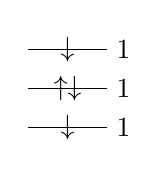
\begin{tikzpicture}[baseline={(current bounding box.center)}]
\draw (0,-.5)--node{$\downarrow$}(1,-.5)node[right]{1};
\draw (0,0)--node{$\uparrow\downarrow$}(1,0)node[right]{1};
\draw (0,.5)--node{$\downarrow$}(1,.5)node[right]{1};
\end{tikzpicture}
\end{align*}
能量中的单电子部分为$h_{11}, 2h_{22}, h_{33}$. 
库伦部分为$J_{22}, J_{13}, 2J_{12}, 2J_{23}$. 
交换作用的部分为$-K_{23}, -K_{12}, -K_{13}$. 
那么总能量就是$ h_{11} + 2h_{22} + h_{33} + J_{22} + J_{13} + 2J_{12} + 2J_{23} - K_{23} -K_{12} -K_{13}  $.

\exercise{
直接看出如下几个行列式的能量, 
并与后面给出的式子对照.

\begin{align*}
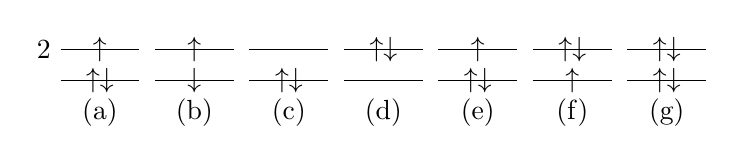
\begin{tikzpicture}[baseline={(current bounding box.center)}]
%=======subfigure(a)=============
\draw (0,.4)node[left]{2}--node{$\uparrow$}+(1,0);
\draw (0,0)--node{$\uparrow\downarrow$}+(1,0);
\draw (.5,-.4)node{(a)};
%=======subfigure(b)=============
\draw (1.2,.4)--node{$\uparrow$}+(1,0);
\draw (1.2,0)--node{$\downarrow$}+(1,0);
\draw (1.7,-.4)node{(b)};
%=======subfigure(c)=============
\draw (2.4,.4)--node{}+(1,0);
\draw (2.4,0)--node{$\uparrow\downarrow$}+(1,0);
\draw (2.9,-.4)node{(c)};
%=======subfigure(d)=============
\draw (3.6,.4)--node{$\uparrow\downarrow$}+(1,0);
\draw (3.6,0)--node{}+(1,0);
\draw (4.1,-.4)node{(d)};
%=======subfigure(e)=============
\draw (4.8,.4)--node{$\uparrow$}+(1,0);
\draw (4.8,0)--node{$\uparrow\downarrow$}+(1,0);
\draw (5.3,-.4)node{(e)};
%=======subfigure(f)=============
\draw (6,.4)--node{$\uparrow\downarrow$}+(1,0);
\draw (6,0)--node{$\uparrow$}+(1,0);
\draw (6.5,-.4)node{(f)};
%=======subfigure(g)=============
\draw (7.2,.4)--node{$\uparrow\downarrow$}+(1,0);
\draw (7.2,0)--node{$\uparrow\downarrow$}+(1,0);
\draw (7.7,-.4)node{(g)};
\end{tikzpicture}
\end{align*}
a. $h_{11} + h_{22} + J_{12} - K_{12}$

b. $h_{11} + h_{22} + J_{12}$

c. $2h_{11}+ J_{11} $

d. $2h_{22}+ J_{22} $

e. $2h_{11}+ h_{22} + J_{11} + 2J_{12} - K_{12}$

f. $2h_{22}+ h_{11} + J_{22} + 2J_{12} - K_{12}$

g. $2h_{11}+ 2h_{22}+ J_{11} + J_{22} + 4J_{12} - 2K_{12}$
}

\section{二次量子化}
\label{sec2.4}
反对称原理是量子力学中的一个公理, 
不用说, 
薛定谔方程本身也是量子力学公理之一. 
我们之前已经通过Slater行列式及其线性组合来保证波函数满足这个原理. 
那么能否用Slater行列式以外的办法来满足反对称原理呢?二次量子化就是这样一种框架, 
在这个框架下波函数的反对称性质被转化为一些算子的代数性质. 
二次量子化中不包含新的物理, 
它只是另外一种处理多电子体系的办法, 
虽然这个办法相当优雅. 
借助二次量子化, 
我们可以把重心从$N$-电子波函数本身上移开, 
转而关注之前研究过的单双电子积分$\braket{i|h|j}, \braket{ij|kl}$. 
二次量子化在与多电子问题相关的文献中由广泛应用. 
这里讲述二次量子化不仅是提供一种推导之前所得结果的额外办法, 
更是为接触这些文献作准备. 
本书其余章节并未一般性地使用二次量子化, 
因此本节可以选读.

\subsection{产生、湮灭算符及其反对易关系}
\label{sec2.4.1}
我们从行列式出发, 
展示行列式的性质可以转换为算符的代数性质, 
逐步构建二次量子化框架. 
首先我们为每个自旋轨道$\chi_i$配上一个\emph{产生}算符, 
用它作用于任意行列式$\ket{\chi_k\cdots\chi_l}$上产生的效果来定义这个算符本身, 
作用效果如下
\begin{align}\label{eq:2.190}
a_i^\dagger \ket{\chi_k\cdots\chi_l} = \ket{\chi_i\chi_k\cdots\chi_l}
\end{align}
因此$\cs_i$的效果就是在自旋轨道$\chi_i$上产生一个电子. 
两个产生算符作用到行列式上时, 
作用顺序很重要. 
考虑
\begin{align}\label{eq:2.191}
\cs_i\cs_j\ket{\chi_k\cdots\chi_l} = \cs_i \ket{\chi_j\chi_k\cdots\chi_l} = \ket{\chi_i\chi_j\chi_k\cdots\chi_l}
\end{align}
另一方面
\begin{align}\label{eq:2.192}
\cs_j\cs_i\ket{\chi_k\cdots\chi_l} = \cs_j\ket{\chi_i\chi_k\cdots\chi_l} & = \ket{\chi_j\chi_i\chi_k\cdots\chi_l}\notag\\
& = - \ket{\chi_i\chi_j\chi_k\cdots\chi_l}
\end{align}
其中用到了Slater行列式的反对称性质(见\autoref{2.40}). 
将\autoref{eq:2.191}、\autoref{eq:2.192}加起来可得
\begin{align}
(\cs_i\cs_j + \cs_j\cs_i)\ket{\chi_k\cdots\chi_l} = 0
\end{align}
由于$\ket{\chi_k\cdots\chi_l}$可以是任意行列式, 
所以可得一个算符之间的关系:
\begin{align}\label{eq:2.194}
\cs_i\cs_j + \cs_j\cs_i = 0 = \{ \cs_i, \cs_j \}
\end{align}
其中使用了之前引入的两个算符的\emph{反对易子}记号(见见\autoref{eq:1.19a}). 
由于
\begin{align}
\cs_i\cs_j = - \cs_j\cs_i
\end{align}
我们可以利用这个性质来交换两个产生算符的顺序——只要记得改变符号就行. 
若$i=j$, 
则有
\begin{align}
\cs_i\cs_i = - \cs_i\cs_i = 0
\end{align}
这就是说, 
无法在一个自旋轨道上产生两个电子(Pauli排斥原理). 
因此
\begin{align}
\cs_1\cs_1\ket{\chi_2\chi_3} = \cs_1\ket{\chi_1\chi_2\chi_3} = \ket{\chi_1\chi_1\chi_2\chi_3 = 0}
\end{align}
更一般地
\begin{align}
\cs_i \ket{\chi_k\cdots\chi_l} = 0,\quad\text{若} i\in \{ k,\cdots, l \}
\end{align}
也就是说, 
如果自旋轨道$\chi_i$上已有一个电子, 
那么就无法再于$\chi_i$上产生一个电子.

\exercise{
请用行列式的性质证明
\begin{align*}
(\cs_1\cs_2 + \cs_2\cs_1)\ket{K} = 0
\end{align*}
其中$\ket{K}$是以下行列式中的任意一个$\{ \ket{\chi_1\chi_2}, \ket{\chi_1\chi_3}, \ket{\chi_1\chi_4}, \ket{\chi_2\chi_3}, \ket{\chi_2\chi_4}, \ket{\chi_3\chi_4}, \}$
}
现在引进\emph{湮灭算符} $a_i$. 
它是产生算符$\cs_i$的伴随算符(adjoint operator)(即$(\cs_i)^\dagger = a_i$). 
和\autoref{eq:2.190}的精神类似, 
$a_i$按下式定义:
\begin{align}\label{eq:2.199}
a_i \ket{\chi_i\chi_k\cdots\chi_l} = \ket{\chi_k\cdots\chi_l}
\end{align}
那么$a_i$的作用就是在$\chi_i$上挪去或者湮灭一个电子. 
注意湮灭算符作用在行列式上时, 
若想湮灭某个自旋轨道上的电子, 
该自旋轨道必须在行列式的最左边. 
如果自旋轨道不在合适的位置上, 
则必须交换行列式中的列, 
以将自旋轨道放在合适的位置:
\begin{align}
a_i \ket{\chi_k\chi_l\chi_i} = -a_i \ket{\chi_i\chi_l\chi_k} = -\ket{\chi_l\chi_k} = \ket{\chi_k\chi_l}
\end{align} 

那么, 
为什么湮灭算符被定义为产生算符的伴随算符?考虑如下行列式
\begin{align}
\ket{K} = \ket{\chi_i\chi_j}
\end{align}
很明显
\begin{align}
\ket{K} = \cs_i \ket{\chi_j} 
\end{align}
取上式的伴随, 
则有(见\autoref{eq:1.52}\autoref{eq:1.57})
\begin{align}\label{eq:2.203}
\bra{K} = \bra{\chi_j}(\cs_i)^\dagger = \bra{\chi_j}a_i
\end{align}
用$\ket{K}$右乘\autoref{eq:2.203},就有
\begin{align}
\braket{K|K} = \braket{\chi_j|a_j|K}
\end{align}
由于$\braket{K|K} = 1 = \braket{\chi_j|\chi_j}$, 
只有当下式成立时, 
我们的框架才是自洽的:
\begin{align}\label{eq:2.205}
a_i\ket{K} = a_i\ket{\chi_i\chi_j} = \ket{\chi_j}
\end{align} 
这与\autoref{eq:2.199}中湮灭算符的定义相同. 
由\autoref{eq:2.203}可知道, 
$a_i$如果作用再一个放在左边的行列式上, 
其作用于产生算符相同. 
类似, 
$\cs_i$作用在左边的行列式上, 
效果和湮灭算符相同. 
举个例子, 
\autoref{eq:2.205}的伴随就是
\begin{align}
\bra{K}\cs_i = \bra{\chi_j}
\end{align}

为得到湮灭算子的反对易关系, 
我们取\autoref{eq:2.194}的伴随. 
由于(见\autoref{ex:1.3}):
\begin{align}
\left( \mathscr{AB} \right)^\dagger = \mathscr{B}^\dagger\mathscr{A}^\dagger
\end{align} 
那么
\begin{equation}\label{eq:2.208}
a_ja_i + a_ia_j = 0 =\{a_j,a_i\}
\end{equation}
因此
\begin{align}
a_ia_j = -a_ja_i
\end{align}
所以我们能交换两个湮灭算符的顺序, 
只要记得改变符号. 
若$i=j$, 
则
\begin{align}
a_ia_i = -a_ia_i = 0
\end{align}
这就是说无法湮灭一个电子两次. 
推论就是无法从一个本来没有电子占据的自旋轨道上挪去一个电子:
\begin{align}
a_i\ket{\chi_k\cdots\chi_l} = 0\quad \text{若 } i\not\in\{k,\ldots,l \}
\end{align}

还未讨论的就是产生算符和湮灭算符之间应该如何交换顺序. 
考虑算符$a_i\cs_i + \cs_ia_i$作用于一任意行列式$\ket{\chi_k\cdots\chi_l}$上. 
若自旋轨道$\chi_i$在这个行列式中并未被电子占据, 
则有
\begin{align}
(a_i\cs_i + \cs_ia_i) \ket{\chi_k\cdots\chi_l} & = a_i\cs_i \ket{\chi_k,\cdots,\chi_l} \notag \\
& = a_i\ket{\chi_i\chi_k\cdots\chi_l} \notag \\
& = \ket{\chi_k\cdots\chi_l}
\end{align}
另一方面, 
若$\chi_i$是一个占据轨道, 
则有
\begin{align}
(a_i\cs_i + \cs_ia_i) \ket{\chi_k\cdots\chi_l} & = \cs_i \ket{\chi_k\cdots\chi_i\cdots\chi_l} \notag \\
& = -\cs_i a_i \ket{\chi_i\cdots\chi_k\cdots\chi_l} \notag \\
& = -\cs_i \ket{\cdots\chi_k\cdots\chi_l} \notag \\
& = \ket{\chi_k\cdots\chi_i\cdots\chi_l}
\end{align}
两种情况下所得的结果一样. 
因此可得算符之间的关系
\begin{align}\label{eq:2.214}
(a_i\cs_i + \cs_ia_i) = 1 = \{ a_i,\cs_i \}
\end{align}
最后来考虑$(\cs_ja_i + a_i\cs_j)\ket{\chi_k\cdots\chi_j}(i\neq j)$. 
这个式子仅当自旋轨道$\chi_i$在行列式中, 
且$\chi_j$不在行列式中时才不为$0$. 
 否则, 
由于$\cs_j$的动作是产生一个电子(而现在已有一个电子在相应轨道上), 
或者$a_i$的试图湮灭一个不存在的电子, 
结果就会是零.
但是, 
即使$i\in\{ k,\ldots,l \}, j\not\in\{ k,\ldots, l \}$, 
结果也会是零, 
因为行列式是反对称的:
\begin{align}
(a_i\cs_j + \cs_ja_i)\ket{\chi_k\cdots\chi_i\cdots\chi_l} & = -(a_i\cs_j + \cs_ja_i) \ket{\chi_i\cdots\chi_k\cdots\chi_l} \notag\\
& = -a_i\ket{\chi_j\chi_i\cdots\chi_k\cdots\chi_l} - \cs_j\ket{\cdots\chi_k\cdots\chi_l} \notag\\
& = a_i\ket{\chi_i\chi_j\cdots\chi_k\cdots\chi_l} - \ket{\chi_j\cdots\chi_k\cdots\chi_l} \notag\\
& = 0
\end{align}
因此就有
\begin{align}
a_i\cs_j + \cs_ja_i = 0 = \{ a_i, \cs_j \}\quad i\neq j
\end{align}
将此式与\autoref{eq:2.214}合在一起就的到了产生算符和湮灭算符的反对易关系:
\begin{align}\label{eq:2.217}
a_i\cs_j + \cs_ja_i = \delta_{ij} = \{ a_i,\cs_j \}
\end{align}
有了这个式子, 
就能按照它来交换产生算符和湮灭算符的次序, 
只要他们关联着的自旋轨道不同, 
即$i\neq j$, 
那么交换时只要变号即可:
\begin{subequations}
    \begin{align}
    a_i\cs_j = -\cs_ja_i\quad i\neq j \\
\intertext{
但需注意, 若这两个算符所关联的自旋轨道相同$(i=j)$, 那么会有如下式子:}
    a_i\cs_i = 1 -\cs_ia_i
    \end{align}
\end{subequations}

\exercise{
请利用行列式的性质证明
\begin{align*}
(a_1\cs_2 + \cs_2a_1 )\ket{K} & = 0\\
(a_1\cs_1 + \cs_1a_1 )\ket{K} & = \ket{K}
\end{align*}
当$\ket{K}$是如下任一个的时候都成立:$\{ \ket{\chi_1\chi_2}, \ket{\chi_1\chi_3}, \ket{\chi_1\chi_4}, \ket{\chi_2\chi_3}, \ket{\chi_2\chi_4}, \ket{\chi_3\chi_4}  \}$.

}

Slater行列式的所有性质都蕴含在这几个反对易关系中, 
这些性质有:一对产生算符的反对易关系(\autoref{eq:2.194})、一对湮灭算符的反对易关系(\autoref{eq:2.208})、 产生算符和湮灭算符之间的反对易关系(\autoref{eq:2.217}). 
为了在二次量子化框架下定义Slater行列式, 
需要引入一个真空态$\ket{\,\,}$. 
所谓真空态, 是系统的一种状态:此时系统内没有任何电子. 进一步规定真空态是归一化的:
\begin{align}
\braket{\,\,|\,\,} = 1
\end{align} 
而且有如下性质:
\begin{align}
a_i \ket{\,\,} = 0 = \bra{\,\,} \cs_i
\end{align}
这个式子的意思是:真空态中没有电子, 
那么就无法从中挪去一个电子. 
若把产生算符连续地作用到真空态上, 
则可以构造处系统的任何态. 
比如
\begin{align}
\ket{\chi_i} = \cs_i\ket{\,\,}
\end{align}
或者更一般地
\begin{align}
\cs_i\cs_k\cdots\cs_i = \ket{\chi_i\chi_k\cdots\chi_l}
\end{align}
这个式子就是二次量子化表象下的Slater行列式. 
从行列式中导出的一切结论同样能用产生算符和湮灭算符的代数性质导出来. 


\autoref{ex:2.5}中曾计算过两个行列式之间的重叠:
\begin{align}\label{eq:2.223}
\ket{K} = \ket{\chi_i\chi_j} = \cs_i\cs_j\ket{\,\,}\\
\ket{L} = \ket{\chi_k\chi_l} = \cs_k\cs_i\ket{\,\,}
\label{eq:2.224}
\end{align}
那里用的办法是将行列式展开, 
再对两个电子的空间坐标和自旋坐标积分, 
使用自旋轨道之间的正交性. 
这里用二次量子化的办法计算这个重叠. 
\autoref{eq:2.223}的伴随是:
\begin{align}
\bra{K} = \bra{\,\,}(\cs_i\cs_j)^\dagger = \bra{\,\,}a_ja_i
\end{align}
由此可知
\begin{align}
\braket{k|L} = \braket{\,,|a_ja_i\cs_k\cs_i|\,\,}
\end{align}
求这个矩阵元的一般策略就是利用反对易关系把湮灭算符挪到最右边, 
这样就和真空态直接接触. 
我们先处理$a_i$. 
由于
\begin{align}
a_i\cs_k = \delta_{ik} - \cs_ka_i
\end{align}
我们有
\begin{align}\nonumber
\braket{K|L} & = \braket{\,\,|a_j(\delta_{ik}-\cs_ka_i)\cs_l|\,\,}\\
             & = \delta_{ik}\braket{\,\,|a_j\cs_l|\,\,} - \braket{\,\,|a_j\cs_ka_i\cs_l|\,\,}
\end{align}
下一步就是将第一项中的$a_j$以及第二项中的$a_i$都挪到靠右的地方, 
得到:
\begin{align}
\braket{K|L} = \delta_{ik}\delta_{jl} \braket{\,\,|\,\,} - \delta_{ik}\braket{\,\,|\cs_la_j|\,\,} - \delta_{il}\braket{\,\,|a_j\cs_k|\,\,} + \braket{\,\,|a_j\cs_k\cs_la_i|\,\,}
\end{align}
上式的第二项和最后项都是一个湮灭算符作用在真空态上, 
其结果为$0$. 
最后一步就是把第三项中的$a_j$挪到最右:
\begin{align}
\braket{K|L} & = \delta_{ik}\delta_{jl} \braket{\,\,|\,\,} - \delta_{il}\delta_{jk}\braket{\,\,|\,\,} + \delta_{il}\braket{\,\,|\cs_ka_j|\,\,}\notag\\
& = \delta_{jk}\delta_{jl} - \delta_{il}\delta_{jk}
\end{align}
第二个等号是由于真空态已预先规定为归一化的. 
这里所得的结果于\autoref{ex:2.5}中的相同. 

\exercise{
用二次量子化的办法证明$\braket{\chi_i|\chi_j} = \delta_{ij}$.

\Next
设想一个态
\begin{align*}
\ket{K} = \ket{\chi_1\chi_2\cdots\chi_N} = \cs_1\cs_2\cdots\cs_N\ket{\,\,}
\end{align*}
请证明在$i=j, i\in\{ 1,2,\ldots,N \}$的条件下, 
$\braket{K|\cs_i\cs_j|K}=1$.

\Next
令$\ket{\Psi_0} = \ket{\chi_1\cdots\chi_a\chi_b\cdots\chi_N}$为一Hartree-Fock基态. 
请证明
\begin{enumerate}[{a.}]
	\setlength{\itemsep}{0pt}
	\item $a_r\ket{\Psi_0} = 0 = \bra{\Psi_0}\cs_r$.
	\item $\cs_a\ket{\Psi_0} = 0 = \bra{\Psi_0}a_a$.
	\item $\ket{\Psi_0} = \cs_ra_a\ket{\Psi_0}$.
	\item $\bra{\psi_a^r} = \bra{\Psi_0}\cs_aa_r$.
	\item $\ket{\Psi_{ab}^{rs}} = \cs_sa_b\cs_ra_a\ket{\Psi_0} = \cs_r\cs_sa_ba_a\ket{\Psi_{0}}$.
	\item $\bra{\Psi_{ab}^{rs}} = \bra{\Psi_0}\cs_aa_r\cs_ba_s = \bra{\Psi_0}\cs_a\cs_ba_s a_r$.
\end{enumerate}
}
\subsection{二次量子化算符及其矩阵元}
\label{sec2.4.2}
到此我们已经了解, 
行列式可由产生算符、湮灭算符、真空态来表示. 
这些算符满足一组反对易关系. 
目前所建立的就是一种满足反对称原理的多电子波函数的表象, 
操作此表象完全不用借助行列式的性质. 
为了完成这个不借助行列式的多电子体系的理论, 
须将多电子算符$\mathcal{O}_1,\mathcal{O}_2$也用产生湮灭算符表示. 
有一点是确定的, 
二次量子化表象下正确的$\mathcal{O}$, 
其矩阵元$\braket{K|\mathcal{O}|L}$无论是用行列式的性质求, 
还是用算符的代数性质来求, 
数值必须相同. 
$\mathcal{O}_1$(或单电子算符之和)与$\mathcal{O}_2$(或电子间的总的库伦排斥算符)正确的二次量子化表达式如下:
\begin{align}
\mathcal{O}_1 & = \sum_{ij} \braket{i|h|j}\cs_ia_j\\
\mathcal{O}_2 & = \frac{1}{2}\sum_{ijkl}\braket{ij|kl}\cs_i\cs_ja_la_k
\end{align}
其中求和遍及整个自旋轨道集合$\{\chi_i\}$. 
有一点要指出, 
在这种形式的算符与电子的数目并无关系, 
而且单、双电子积分都显式地出现在表达式中. 
二次量子化的优点就是体系的电子数目不同时, 
处理方法不变. 
当研究固体时这个形式有很大便利.

\exercise{
令$\Psi_0 = \ket{\chi_1\chi_2} = \cs_1\cs_2\ket{\,\,}$为\phrase{极小基 $\mathrm{H}_2$}的Hartree-Fock波函数. 
请用二次量子化的办法证明
\begin{align*}
\braket{\Psi_0|\mathcal{O}_1|\Psi_0} = \sum_{ij}\braket{i|h|j}\braket{\,,|a_2 a_1 \cs_i a_j \cs_1\cs_2|\,\,}
& = \braket{1|h|1} + \braket{2|h|2}
\end{align*}
}

为说明二次量子化与之前用Slater行列式所得的结果等价, 
现用二次量子化的办法计算Hartree-Fock基态$\ket{\Psi_0} = \ket{\chi_1\cdots\chi_a\chi_v\cdots\chi_N}$的能量. 
对单电子算符之和, 
我们有
\begin{align}
\braket{\Psi_0|\mathcal{O}_1|\Psi_0} = \sum_{ij}\braket{i|h|j}\braket{\Psi_0|\cs_i a_j|\Psi_{0}}
\end{align}
由于上式中$a_j,\cs_i$的作用就是湮灭一个电子($a_j$作用在右边, 
$\cs_i$作用在左边), 
指标$i,j$须在集合$\{a,b,\ldots\}$之内取, 
那么
\begin{align}
\braket{\Psi_0|\mathcal{O}_1|\Psi_0} = \sum_{ab}\braket{a|h|b}\braket{\Psi_0|\cs_a a_b|\Psi_{0}}
\end{align}
利用
\begin{align}
\cs_a a_b = \delta_{ab} - a_b\cs_a \notag
\end{align}
把$\cs_a$挪到右边, 
有
\begin{align}
\braket{\Psi_0|\cs_a a_b|\Psi_0} = \delta_{ab}\braket{\Psi_0|\Psi_0} - \braket{\Psi_0|a_b\cs_a|\Psi_0}
\end{align}
右边第二项为$0$, 
因为$\cs_a$试图在$\chi_a$上产生一个电子, 
而这个$\ket{\Psi_0}$中的轨道已经被电子占据了. 
又由于$\braket{\Psi_0|\Psi_0} = 1$, 
最终结果就是
\begin{align}
\braket{\Psi_0|\mathcal{O}_1|\Psi_0} = \sum_{ab} \braket{a|h|b}\delta_{ab} = \sum_a\braket{a|h|a}
\end{align} 
与\autoref{t2.5}给出的结果完全相同.


对双电子算符之和, 
有
\begin{align}
\braket{\Psi_0|\mathcal{O}_2|\Psi_0} = \frac{1}{2}\sum_{ijkl}\braket{ij|kl}\braket{\Psi_0|\cs_i\cs_ja_ia_k|\Psi_0}
\end{align}
基于和单电子算符那里一样的理由, 
指标$i,j,k,l$应该限制在$\{a,b,\ldots\}$内:
\begin{align}
\braket{\Psi_0|\mathcal{O}_2|\Psi_0} =\frac{1}{2}\sum_{abcd}\braket{ab|cd}\braket{\Psi_0|\cs_a\cs_ba_ca_d|\Psi_0}
\end{align}
然后就是和上面一样的办法:将$\cs_a,\cs_b$挪到右边使其作用到$\ket{\Psi_0}$上:
\begin{align*}
\braket{\Psi_0|\cs_i\cs_ja_ia_k|\Psi_0} = & \delta_{bd}\braket{\Psi_0|\cs_a a_c|\Psi_0} - \braket{\Psi_0|\cs_a a_d \cs_b a_c|\Psi_0} \\
= & \delta_{bd}\delta_{ac}\braket{\Psi_0|\Psi_0} - \delta_{bd}\braket{\Psi_0|a_c\cs_a|\Psi_0}\\
& - \delta_{bc}\braket{\Psi_0|\cs_aa_d|\Psi_0} + \braket{\Psi_0|\cs_ia_da_c\cs_b|\Psi_0}\\
= & \delta_{bd}\delta_{ac} - \delta_{bc}\delta_{ad}\braket{\Psi_0|\Psi_{0}} + \delta_{bc}\braket{\Psi_0|a_d\cs_a|\Psi_0}\\
= & \delta_{bd}\delta_{ac} - \delta_{bc}\delta_{ad}
\end{align*}
结果就是两项:第一项中令$c=a,d=b$, 
第二项令$c=b,d=a$, 
就得到与\autoref{t2.6}相同的结果:
\begin{align}
\braket{\Psi_0|\mathcal{O}_2|\Psi_0} = \frac{1}{2}\sum_{ab}\braket{ab|ab} - \braket{ab|ba}
\end{align}
\exercise{
证明:
\begin{align*}
\braket{\Psi_a^r|\mathcal{O}_1|\Psi_0} & = \sum_{ij}\braket{i|h|j}\braket{\Psi_0|\cs_a a_r \cs_i a_j|\Psi_0}\\
& = \braket{r|h|a}
\end{align*}
记得将$\cs_a,a_r$挪到最右.

\Next
证明:
\begin{align*}
\braket{\Psi_a^r|\mathcal{O}_2|\Psi_0} = \sum_a^N\braket{rb||ab}
\end{align*}
\textit{提示:}先证明
\begin{align*}
\braket{\Psi_0|\cs_a a_r\cs_i\cs_j a_l a_k|\Psi_0} =& \delta_{rj}\delta_{al}\braket{\Psi_0|\cs_i a_k|\Psi_0} - \delta_{rj}\delta_{ak}\braket{\Psi_0|\cs_i a_l|\Psi_0}\\
& + \delta_{ri}\delta_{ak}\braket{\Psi_0|\cs_j a_l|\Psi_0} - \delta_{ri}\delta_{al}\braket{\Psi_0|\cs_j a_k|\Psi_0}
\end{align*}
之后可参考\autoref{ex:2.27}.

}
\section{自旋匹配组态}
\label{sec2.5}
之前提到, 
电子的自旋可由两个自旋函数$\alpha(\omega) \equiv \alpha, \beta(\omega) \equiv \beta$来描述. 
本节会更详细地讨论自旋, 
并讨论多电子系统的自旋态. 
会讲述由一组自旋轨道构成的\emph{限制性}Slater行列式:$\alpha$自旋所对应的空间轨道与和$\beta$自旋所对应的相同, 
也即$\{\chi_i\} = \{\psi_i\alpha,\psi_i\beta\}$. 
限制性行列式除了一些特殊情形外, 
都不是总自旋算符的本征函数. 
但可以将行列式恰当地线性组合起来, 
以得到\emph{自旋匹配组态}, 
它是正确的本征函数. 
本节最后会讲述\emph{非限制性}行列式, 
其中的每一对自旋轨道中, 
两个自旋对应的空间轨道是不一样的, 
即$\{\chi_i\} = \{\psi_i^\alpha\alpha,\psi_i^\beta\beta\}$.

\subsection{自旋算符}
\label{sec2.5.1}
单个粒子的自旋角动量算符是矢量算符:
\begin{align}
\vec{s} = s_x\vec{i} + s_y\vec{j} + s_z\vec{k}
\end{align}
此处$\vec{i},\vec{j},\vec{k}$是沿着$x,y,z$方向的单位向量. 
$\vec{s}$的平方则是标量算符:
\begin{align}\label{eq:2.241}
s^2 = \vec{s}\cdot\vec{s} = s^2_x + s^2_y + s^2_z
\end{align}
自旋角动量分量满足如下对易关系:
\begin{align}\label{eq:2.242}
[s_x,s_y] = is_z,\quad [s_y,s_z] = s_x,\quad [s_z,s_x]=is_y
\end{align}
描述单个粒子的完全集可以选为$s^2$及其某个分量的共同本征函数, 
一般将分量选为$s_z$:
\begin{subequations}
	\begin{align}
	s^2\ket{s,m_s} & = s(s+1)\ket{s,m_s}\tag{2.243a}\\
	s_z\ket{s,m_s} & = m_s\ket{s,m_s}\tag{2.243b}
	\end{align}
\end{subequations}
式中$s$是描述总自旋的一个量子数, 
$m_s$是描述自旋$z$分量的量子数. 
$s$的允许值为$0,\frac{1}{2},1,\frac{3}{2},\ldots$, 
$m_s$有$2s+1$个可能值:$-s,-s+1,-s+2,\ldots,s-1,s$. 
对于电子这两个值是$s=\frac{1}{2},m_s=\pm\frac{1}{2}$. 
那么描述电子自旋的完全集为
\begin{subequations}
	\begin{align}
	\ket{\frac{1}{2},\frac{1}{2}} \equiv \ket{\alpha}\\
	\ket{\frac{1}{2},-\frac{1}{2}} \equiv \ket{\beta}
	\end{align}
\end{subequations}
这两个态是$s^2,s_z$的本征态:
\begin{subequations}\label{eq:2.245}
	\begin{align}
	s^2\ket{\alpha} & = \frac{3}{4}\ket{\alpha},\quad s^2\ket{\beta} = \frac{3}{4}\ket{\beta}\\
	s_z\ket{\alpha} & =\frac{1}{2}\ket{\alpha},\quad s_z\ket{\beta} = -\frac{1}{2}\ket{\beta}\\
\intertext{
	但不是$s_x,s_y$的本征态:}
	s_x\ket{\alpha} & = \frac{1}{2}\ket{\beta},\quad s_x\ket{\beta} = \frac{1}{1}\ket{\alpha}\\
	s_y\ket{\alpha} & =\frac{i}{2}\ket{\beta},\quad s_y\ket{\beta} = -\frac{i}{2}\ket{\alpha}
	\end{align}
\end{subequations}
我们平常不太使用$s_x,s_y$, 
而是用更好用的阶梯算符:``上升”算符$s_+$, 
``下降”算符$s_-$,

\begin{subequations}
	\begin{align}
	s_+ = s_x + is_y\\
	s_- = s_x - is_y
	\end{align}
\end{subequations}
这两个算符可以升降$m_s$的值, 
作用一次, 
$m_s$的值改变$1$:
\begin{subequations}\label{eq:2.247}
	\begin{align}
	s_+\ket{\alpha} = 0,\quad s_+\ket{\beta} = \ket{\alpha}\\
	s_-\ket{\alpha} = \ket{\beta},\quad s_-\ket{\beta} = 0\\
	\end{align}
\end{subequations}
用\autoref{eq:2.242}中的对易关系, 
可将\autoref{eq:2.241}中的$s^2$的表达式改写为:
\begin{subequations}\label{eq:2.248}
	\begin{align}
	s^2 = s_+s_- - s_z + s_z^2\\
	s^2 = s_-s_+ + s_z + s_z^2 
	\end{align}
\end{subequations}
\exercise{
a) 由\autoref{eq:2.245}导出\autoref{eq:2.247}; b)推导式\autoref{eq:2.248}.
\Next
求出$s^2,s_z,s_+,s_-$在$\ket{\alpha},\ket{\beta}$为基时的矩阵表示. 
验证式(2.248a,b)的矩阵表示.

\Next
用\autoref{eq:2.242}中的反对易关系证明$[s^2,s_z]=0$.

}

多电子体系的总自旋算符就是每个电子自旋算符的矢量和:
\begin{align}
\vec{\mathscr{S}} = \sum_{i=1}^{N}\vec{s}(i)
\end{align}
由此式可以看出, 
总自旋的分量以及阶梯算符就是对应的单电子算符之和:
\begin{subequations}
	\begin{align}
	\ts_I   & = \sum_{i=1}^{N}s_I(i)\quad I=x,y,z\\
	\ts_\pm & = \sum_{i=1}^{N}s_\pm(i) 
	\end{align}
\end{subequations}
总自旋的平方为
\begin{align}
\ts^2 & = \vec{\ts}\cdot\vec{\ts} = \sum_{i=1}^{N}\sum_{j=1}^{N} \vec{s}(i)\cdot\vec{s}(j) \notag \\
      & = \ts_+\ts_- - \ts_z + \ts^2_z\notag\\
      & = \ts_-\ts_+ + \ts_z + \ts^2_z
\end{align}
它就是对应的单电子算符(对角项$i=j$)之和加上双电子算符(交叉项$i\neq j$)之和.


在通常的非相对论处理下(本书即如此), 
哈密顿量中并无自旋坐标, 
因此$\ts^2,\ts_z$都与哈密顿量对易:
\begin{align}
[\hs,\ts^2] = 0 = [\hs,\ts_z]
\end{align} 
那么, 
哈密顿量的精确本征函数也就是这两个自旋算子的本征函数:
\begin{subequations}
	\begin{align}
	\ts^2\ket{\Phi} & = S(S+1)\ket{\Phi}\\
	\ts_z\ket{\Phi} & = M_S\ket{\Phi}
	\end{align}
\end{subequations}
式中$S,M_S$分别是$N$-电子态$\ket{\Phi}$的总自旋量子数及其分量. 
总自旋为$S=0,\frac{1}{2},1,\frac{3}{2},\ldots$的态, 
其多重度为$(2S+1)=1,2,3,4$, 
我们分别把这些态称作单重态、双重态、三重态、四重态等等. 
\sch 方程的近似解并不一定是纯自旋态. 
但是将近似波函数限制为单重、双重、三重态等等会比较方便.


所有的单行列式都是$\ts_z$的本征函数(见\autoref{ex:2.37}). 
写出来就是
\begin{align}
\label{eq:2.254}
\ts_z\ket{\chi_i\chi_j\cdots\chi_k} = \frac{1}{2}(N^\alpha - N_\beta)\ket{\chi_i\chi_j\cdots\chi_k} = M_S\ket{\chi_i\chi_j\cdots\chi_k}
\end{align}
式中$N^\alpha$是具有$\alpha$自旋的轨道数目, 
$N^\beta$是具有$\beta$自旋的轨道数目. 
但要注意, 
单行列式并不一定是$\ts^2$的本征函数. 
正如我们在下一小节要讨论的那样, 
通过几个行列式的线性组合, 
可以构造出自旋匹配组态, 
即$\ts^2$的正确的本征函数.

\exercise{
考虑一个算符$\mathscr{A}$, 
它与哈密顿量对易. 
设$\ket{\Phi}$是$\hs$的本征函数, 
本征值为$E$. 
证明$\mathscr{A}\ket{\Phi}$也是$\hs$的本征函数, 
对应本征值为$E$. 
如果$\ket{\Phi}$是(能量上的)非简并态, 
那么$\mathscr{A}\ket{\Phi}$就是$\ket{\Phi}$的倍数(即$\mathscr{A}\ket{\Phi} = a\ket{\Phi}$). 
那么$\ket{\Phi}$就是$\mathscr{A}$的本征函数. 
若存在简并, 
可以用$\mathscr{H}$的简并本征函数的线性组合构造出$\mathscr{A}$的本征函数. 

\Next
设想厄米算符$\mathscr{A}$与$\hs$对易, 
它的两个非简并本征函数为$\ket{\Phi_{1}},\ket{\Phi_2}$, 
即$\mathscr{A}\ket{\Phi_1} = a_1\ket{\Phi_1},\mathscr{A}\ket{\Phi_2} = a_2\ket{\Phi_2}, a_1\neq a_2$. 
请证明$\ket{\Phi_1|\hs|\Phi_2} = 0$. 
由此可知, 
哈密顿量在单重、三重态组态(仅举一例)之间的矩阵元为0.

\Next
证明\autoref{eq:2.254}. 
\textit{提示:}使用式\autoref{eq:2.115}将Slater行列式展开, 
并注意到$\ts_z$与$\mathscr{P}_n$对易, 
因为$\ts_z$在对电子指标的任意置换下都不变.

}

\subsection{限制性行列式与自旋匹配组态}
\label{sec2.5.2}
\autoref{sec2.2.1}中已经提过, 
给定一组$K$个正交的空间轨道$\{\psi_i|i=1,2,\ldots,K\}$, 
可以构造$2K$个自旋轨道$\{\chi_i|i=1,2,\ldots,2K\}$, 
每个空间轨道乘以$\alpha$或$\beta$即可:
\begin{align}\label{eq:2.255}
\chi_{2i-1}(\mathbf{x}) & = \psi_i(\mathbf{r})\alpha(\omega) \notag\\
\chi_{2i}(\mathbf{x})   & = \psi_i(\mathbf{r})\beta(\omega)
\end{align}
这些自旋轨道称为\emph{限制性}自旋轨道, 
用这些轨道构成的行列式称为限制性行列式. 
在这样的行列式内, 

\begin{figure}[H]
	\centering
	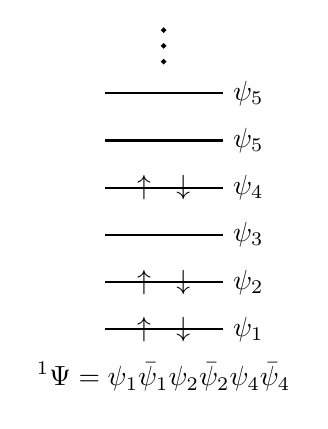
\begin{tikzpicture}[thick]
	%=========== figure left, from bottom to top===========================
	\draw (.75, -.6)node{$\displaystyle \ket{^1\Psi} = \ket{\psi_1\bar{\psi}_1\psi_2\bar{\psi}_2\psi_4\bar{\psi}_4}$};
	\draw (0,0)--++(.5,0)node{$\uparrow$}-- ++(.5,0)node{$\downarrow$}-- ++(.5,0)node[right]{$\psi_1$};
	\draw (0,.6)--++(.5,0)node{$\uparrow$}-- ++(.5,0)node{$\downarrow$}-- ++(.5,0)node[right]{$\psi_2$};
	\draw (0,1.2)--++(.5,0)--node{} ++(.5,0)node{}-- ++(.5,0)node[right]{$\psi_3$};
	\draw (0,1.8)--++(.5,0)node{$\uparrow$}-- ++(.5,0)node{$\downarrow$}-- ++(.5,0)node[right]{$\psi_4$};
	\draw (0,2.4)--++(.5,0)node{}-- ++(.5,0)node{}-- ++(.5,0)node[right]{$\psi_5$};
	\draw (0,3)--++(.5,0)node{}-- ++(.5,0)node{}-- ++(.5,0)node[right]{$\psi_5$};
	\filldraw (0.75,3.4)circle(.5pt) (.75,3.6)circle(.5pt) (.75,3.8)circle(.5pt);
	\end{tikzpicture}
	\caption{一个单重态限制性行列式.}
\end{figure}
一个空间轨道$\psi_i$既可以由单个电子占据(自旋上下都可以), 也能被两个电子占据(自旋一上一下). 非限制性行列式可以按照单占据轨道的数目来分类. 所有轨道都被两个电子占据的行列式称为\emph{闭壳层}行列式. 一个\emph{开壳层}就代表一个仅含一个电子的空间轨道. 可以按照开壳层的数目来称呼行列式.

闭壳层行列式中的所有电子都配对, 
那么很自然, 
闭壳层行列式就是一个纯自旋单态. 
也即, 
它是$\ts^2$的本征函数, 
本征值为零:
\begin{align}\label{eq:2.256}
\ts^2\ket{\psi_i\bar{\psi}_i\psi_j\bar{\psi}_j} = 0(0+1)\ket{\psi_i\bar{\psi}_i\psi_j\bar{\psi}_j} = 0
\end{align}
可见\autoref{ex:2.38} 
最简单的闭壳层行列式就是\phrase{极小基 $\mathrm{H}_2$}的Hartree-Fock基态波函数:
\begin{align}\label{eq:2.257}
\ket{\Psi_0} = \ket{\psi_1\bar{\psi}_1} = [\psi_1(1)\psi_1(2)]^{-1/2}(\alpha(1)\beta(2) - \beta(1)\alpha(2))
\end{align}
式中最后的等号就是将行列式展开. 
这个波函数的自旋部分就是一双电子系统的单重自旋函数. 
同样, 
双激发态$\ket{\Psi_{1\bar{1}}^{2\bar{2}}}$也是单重态.

\exercise{
证明\autoref{eq:2.256}. 
\textit{提示:}1) $\ts^2 = \ts_-\ts_+ + \ts_z + \ts^2_z$, 
2) 用\autoref{eq:2.254}即可证明$\ts_+\ket{\psi_i\bar{\psi}_i}=0$, 
3)
用\autoref{eq:2.115}展开行列式, 
注意到$\ts_+$与置换算符对易, 
4)最后一步, 
$s_+\psi\beta = \psi_\alpha$, 
但行列式此式为0, 
因为其中有相同的两列.

}

现来看开壳层限制性行列式. 
开壳层行列式\emph{不是}$\ts^2$的本征函数, 
除非所有开壳层电子的自旋都平行, 
如\autoref{fig:2.12}中那样. 
举个例子, 
考虑\phrase{极小基 $\hd$}的四个单激发行列式(见\autoref{eq:2.76}, 
四个都是开壳层行列式). 
其中的两个
\begin{subequations}\label{eq:2.258}
	\begin{align}
	\ket{\Psi_1^{\bar{2}}} & = \ket{\bar{2}\bar{1}} = -2^{-1/2}[\psi_1(1)\psi_2(2) - \psi_2(1)\psi_1(2)]\beta(1)\beta(2)\\
	\ket{\Psi_{\bar{1}}^2} & = \ket{12}  = -2^{-1/2}[\psi_1(1)\psi_2(2) - \psi_2(1)\psi_1(2)]\alpha(1)\alpha(2)
	\end{align}
\end{subequations} 
是$\ts^2$的本征函数, 
本征值为$1(1+1)=2$, 
都是三重态. 
另一方面, 
剩下的两个行列式
\begin{subequations}\label{eq:2.259}
	\begin{align}
	\ket{\Psi_1^2} & = \ket{2\bar{1}}\\
	\ket{\Psi_{\bar{1}}^{\bar{2}}} & = \ket{1\bar{2}}
	\end{align}
\end{subequations} 
不是纯自旋态. 
但若对这两个行列式进行恰当的线性组合, 
就可以构造出自旋匹配组态, 
那也就成为$\ts^2$的本征函数. 
具体而言, 
单重的自旋匹配组态可以如此构造:
\begin{align}
\ket{^1\Psi_1^2} & = 2^{-1/2}(\ket{\Psi_{\bar{1}}^{\bar{2}}} + \ket{\Psi_1^2}) \notag\\
& =2^{-1/2}(\ket{1\bar{2}} + \ket{2\bar{1}})\notag \\
	& =2^{-1/2}[ \psi_1(1)\psi_2(2) + \psi_1(2)\psi_2(1)] 2^{-1/2}(\alpha(1)\beta(2) - \beta(1)\alpha(2)) \label{eq:2.260}
\end{align}
三重的自旋匹配组态构造如下
\begin{align}
\ket{^3\Psi_1^2} & = 2^{-1/2}(\ket{\Psi_{\bar{1}}^{\bar{2}}} - \ket{\Psi_1^2}) \notag\\
& =2^{-1/2}(\ket{1\bar{2}} - \ket{2\bar{1}})\notag \\
& =2^{-1/2}[ \psi_1(1)\psi_2(2) - \psi_1(2)\psi_2(1)] 2^{-1/2}(\alpha(1)\beta(2) + \beta(1)\alpha(2))
\end{align}

\begin{figure}[H]
	\centering
	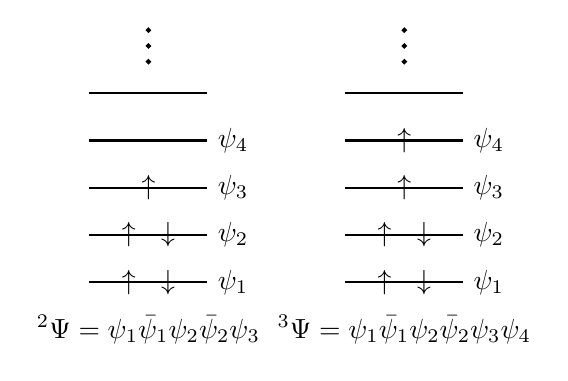
\begin{tikzpicture}[thick]
	%=========== figure left, from bottom to top===========================
	\draw (.75, -.6)node{$\displaystyle \ket{^2\Psi} = \ket{\psi_1\bar{\psi}_1\psi_2\bar{\psi}_2\psi_3}$};
	\draw (0,0)--++(.5,0)node{$\uparrow$}-- ++(.5,0)node{$\downarrow$}-- ++(.5,0)node[right]{$\psi_1$};
	\draw (0,.6)--++(.5,0)node{$\uparrow$}-- ++(.5,0)node{$\downarrow$}-- ++(.5,0)node[right]{$\psi_2$};
	\draw (0,1.2)--++(.5,0)--node{$\uparrow$} ++(.5,0)node{}-- ++(.5,0)node[right]{$\psi_3$};
	\draw (0,1.8)--++(.5,0)node{}-- ++(.5,0)node{}-- ++(.5,0)node[right]{$\psi_4$};
	\draw (0,2.4)--++(.5,0)node{}-- ++(.5,0)node{}-- ++(.5,0);
	\filldraw (0.75,2.8)circle(.5pt) (.75,3)circle(.5pt) (.75,3.2)circle(.5pt);
	%=========== figure left, from bottom to top===========================
	\draw (4,-.6)node{$\displaystyle \ket{^3\Psi} = \ket{\psi_1\bar{\psi}_1\psi_2\bar{\psi}_2\psi_3\psi_4}$};
	\draw (3.25,0)--++(.5,0)node{$\uparrow$}-- ++(.5,0)node{$\downarrow$}-- ++(.5,0)node[right]{$\psi_1$};
	\draw (3.25,.6)--++(.5,0)node{$\uparrow$}-- ++(.5,0)node{$\downarrow$}-- ++(.5,0)node[right]{$\psi_2$};
	\draw (3.25,1.2)--++(.5,0)--node{$\uparrow$} ++(.5,0)node{}-- ++(.5,0)node[right]{$\psi_3$};
	\draw (3.25,1.8)--++(.5,0)--node{$\uparrow$} ++(.5,0)node{}-- ++(.5,0)node[right]{$\psi_4$};
	\draw (3.25,2.4)--++(.5,0)node{}-- ++(.5,0)node{}-- ++(.5,0);
	\filldraw (4,2.8)circle(.5pt) (4,3)circle(.5pt) (4,3.2)circle(.5pt);
	\end{tikzpicture}
	\caption{双重和三重限制性行列式.}
        \label{fig:2.12}
\end{figure}
真如我们所期望的, 
$\ket{^1\Psi_1^2}$的自旋部分和闭壳层波函数\autoref{eq:2.257}相同, 
因为二者都是单重态.

\exercise{
用此式$\ts^2 = \ts_-\ts_+ + \ts_z + \ts^2_z$证明$\ket{^1\psi^2_1}$式单态, 
$\ket{^3\Psi_1^2}$和$\ket{\Psi_{\bar{1}}^2}$是三态.

\Next
证明
\begin{align*}
\braket{^2\Psi_1^2|\hs|^1\Psi_1^2} = h_{11} + h_{22} + J_{12} + K_{12}\\
\braket{^3\Psi_1^2|\hs|^3\Psi_1^2} = h_{11} + h_{22} + J_{12} - K_{12}
\end{align*}
由此三重态的能量就闭单重态能量低. 
请用波函数的空间部分解释此现象.

}

下面将刚才所得的\phrase{极小基 $\hd$}的结果推广. 
第四章和第五章会用到单重自旋匹配组态, 
它由如下闭壳层Hatree-Fock基态的单激发和双激发组成:
\begin{align}
\ket{\Psi_0} = \ket{1\bar{1}\cdots a\bar{a} b\bar{b}}
\end{align}
到底怎么找到办法来把单激发和双激发行列式线性组合为正确的自旋匹配组态就超出了本书的范围;
我们仅引用这些结果. 
构建自旋本征函数的办法非常多. 

对这些方法的一个权威且清晰的描述由Paunz\endnote{R. Paunz, \textit{Spin Eigenfunctions}, Plenum, New York, 1979.}给出.


由单激发态(一个电子由$\psi_a$激发到$\psi_r$)可以构建一个单重自旋匹配组态:
\begin{align}
\ket{^1\Psi_a^r} = 2^{-1/2}(\ket{\Psi_{\bar{a}}^{\bar{r}}} + \ket{\Psi_a^r})
\end{align}
若$a=1,b=2$则上面的式子就退化为\phrase{极小基 $\hd$}的情形, 
即\autoref{eq:2.260}.


对双激发而言, 
可能的单重自旋匹配组态很多, 
结果已列在\autoref{t2.7}中. 
若同一空间轨道的两个电子共同激发到另外一个空间轨道上, 
由这种激发态构成的单重自旋匹配组态记为$\ket{^1\Psi_{aa}^{rr}}$. 
同一空间轨道上的两个电子激发到了不同的空间轨道上, 
由这种激发态构成的单重自旋匹配组态记为$\ket{^1\Psi_{aa}^{rs}}$. 
不同空间轨道的两个电子激发到同一空间轨道, 
由这种激发态构成的单重自旋匹配组态记为$\ket{^1\Psi_{ab}^{rr}}$. 
最后一个, 
不同空间轨道的两个电子激发到不同的空间轨道时, 
有两个线性无关的单重自旋匹配组态, 
记为$\ket{^A\Psi_{ab}^{rs}}, \ket{^B\Psi_{ab}^{rs}}$.


\begin{table}[h]
    \centering
    \caption{\bf 双激发单重自旋匹配组态}
    \label{t2.7}
	\begin{tabular}{ll}
            \hline \\
		%============ 1 ===============
		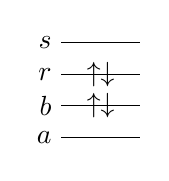
\begin{tikzpicture}[baseline={(current bounding box.center)}]
		\draw (0, 0)node[left]{$a$}--++(.5,0)--++(.5,0);
		\draw (0,.4)node[left]{$b$}--++(.5,0)node{$\uparrow\downarrow$}--++(.5,0);
		\draw (0,.8)node[left]{$r$}--++(.5,0)node{$\uparrow\downarrow$}--++(.5,0);
		\draw (0,1.2)node[left]{$s$}--++(.5,0)--++(.5,0);
		\end{tikzpicture}
		& ${\ket{^1\Psi_{aa}^{rr}}} = \ket{\Psi_{a\bar{a}}^{r\bar{r}}}$\\
		%============ 2 ===============
		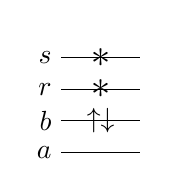
\begin{tikzpicture}[baseline={(current bounding box.center)}]
		\draw (0, 0)node[left]{$a$}--++(.5,0)--++(.5,0);
		\draw (0,.4)node[left]{$b$}--++(.5,0)node{$\uparrow\downarrow$}--++(.5,0);
		\draw (0,.8)node[left]{$r$}--++(.5,0)node{\raisebox{-15pt}{\Large*}}--++(.5,0);
		\draw (0,1.2)node[left]{$s$}--++(.5,0)node{\raisebox{-15pt}{\Large*}}--++(.5,0);
		\end{tikzpicture}
		& ${\ket{^1\Psi_{aa}^{rs}}} = 2^{-1/2}(\ket{\Psi_{a\bar{a}}^{r\bar{s}}} + \ket{\Psi_{a\bar{a}}^{s\bar{r}}})$\\
		%============ 3 ===============
		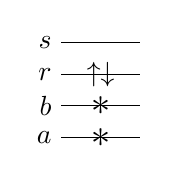
\begin{tikzpicture}[baseline={(current bounding box.center)}]
		\draw (0, 0)node[left]{$a$}--++(.5,0)node{\raisebox{-15pt}{\Large*}}--++(.5,0);
		\draw (0,.4)node[left]{$b$}--++(.5,0)node{\raisebox{-15pt}{\Large*}}--++(.5,0);
		\draw (0,.8)node[left]{$r$}--++(.5,0)node{$\uparrow\downarrow$}--++(.5,0);
		\draw (0,1.2)node[left]{$s$}--++(.5,0)--++(.5,0);
		\end{tikzpicture}
		& ${\ket{^1\Psi_{ab}^{rr}}} = 2^{-1/2}(\ket{\Psi_{a\bar{b}}^{\bar{r}r}} + \ket{\Psi_{a\bar{b}}^{r\bar{r}}}$\\
		%============ 4 ===============
		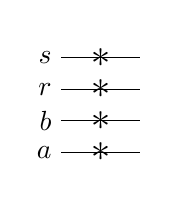
\begin{tikzpicture}[baseline={(current bounding box.center)}]
		\draw (0, 0)node[left]{$a$}--++(.5,0)node{\raisebox{-15pt}{\Large*}}--++(.5,0);
		\draw (0,.4)node[left]{$b$}--++(.5,0)node{\raisebox{-15pt}{\Large*}}--++(.5,0);
		\draw (0,.8)node[left]{$r$}--++(.5,0)node{\raisebox{-15pt}{\Large*}}--++(.5,0);
		\draw (0,1.2)node[left]{$s$}--++(.5,0)node{\raisebox{-15pt}{\Large*}}--++(.5,0);
		\end{tikzpicture}
		& 
		$\begin{aligned}
		{\ket{^A\Psi_{ab}^{rs}}} &= (12)^{-1/2}(2\ket{\Psi_{ab}^{rs}} + 2\ket{\Psi_{\bar{ab}}^{\bar{rs}}} - \ket{\Psi_{\bar{a}b}^{\bar{s}r}} + \ket{\Psi_{\bar{a}b}^{\bar{r}s}} + \ket{\Psi_{a\bar{b}}^{r\bar{s}}} - \ket{\Psi_{a\bar{b}}^{s\bar{r}}}\\
		{\ket{^B\Psi_{ab}^{rs}}} & = \frac{1}{2}(\ket{\Psi_{\bar{a}b}^{\bar{s}r}} + \ket{\Psi_{\bar{a}b}^{\bar{r}s}} + \ket{\Psi_{a\bar{b}}^{r\bar{s}}} + \ket{\Psi_{a\bar{b}}^{s\bar{r}}})
		\end{aligned}$
                \\\hline
	\end{tabular}
\end{table}
\subsection{非限制性行列式}
\label{sec2.5.3}
之前讨论的限制性行列式中, 
$\alpha$自旋和$\beta$自旋的空间轨道被限制为相同的. 
举个例子, 
$\mathrm{Li}$原子的限制性Hartree-Fock基态为:
\begin{align}\label{eq:2.264}
\ket{^2\Psi_\mathrm{RHF}} = \ket{\psi_{1s}\bar{\psi}_{1s}\psi_{2s}}
\end{align} 
如\autoref{fig:2.13}所示. 
在这个行列式中, 
$1s\alpha$电子的空间部分和$1s\beta$电子的空间部分被限制为相同的函数. 
这个限制是真实的, 
因为$1s\alpha$电子与$2s\alpha$电子间由交换作用, 
但与$1s\beta$之间没有. 
那么$2s\alpha$电子就会``极化”$1s$壳层. 
$1s\alpha$和$1s\beta$电子感受到的有效势场不相同, 
这两个电子更倾向于待在不同的空间波函数上. 
直觉上我们可以预期, 
如果空间波函数相同这个限制被打开, 
即不同自旋可对应不同的空间轨道:
\begin{align}\label{eq:2.265}
\ket{\Psi_\mathrm{UHF}} = \ket{\psi_{1s}^\alpha\bar{\psi}_{1s}^\beta\psi_{2s}^\alpha}
\end{align}
\begin{figure}[H]
	\centering
	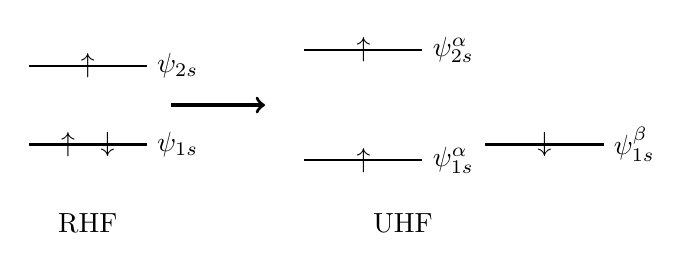
\begin{tikzpicture}[thick]
	\draw (.75,-1)node{RHF};
	\draw (0,0)--++(.5,0)node{$\uparrow$}--++(.5,0)node{$\downarrow$}--++(.5,0)node[right]{$\psi_{1s}$};
	\draw (0,1)--++(.5,0)--node{$\uparrow$}++(.5,0)--++(.5,0)node[right]{$\psi_{2s}$};
	\draw[very thick,->] (1.8,.5)--(3,.5);
	\draw (4.75,-1)node{UHF};
	\draw (3.5,-.2)--++(.5,0)--node{$\uparrow$}++(.5,0)--++(.5,0)node[right]{$\psi_{1s}^\alpha$};
	\draw (3.5,1.2)--++(.5,0)--node{$\uparrow$}++(.5,0)--++(.5,0)node[right]{$\psi_{2s}^\alpha$};
	\draw (5.8,0)--++(.5,0)--node{$\downarrow$}++(.5,0)--++(.5,0)node[right]{$\psi_{1s}^\beta$};
	\end{tikzpicture}
	\caption{将限制性的单行列式放宽为非限制性的单行列式:以$\mathrm{Li}$原子为例.}
        \label{fig:2.13}
\end{figure}
那么得到的能量应当更低. 
事实确实如此. 
波函数\autoref{eq:2.265}是\emph{非限制性}行列式一例. 
它就是$\mathrm{Li}$原子的非限制性基态波函数.


非限制性行列式由非限制自旋轨道构成. 
使用非限制自旋轨道时, 
不同自旋对应不同的空间轨道. 
给定一组$K$个正交归一空间轨道$\{\psi_i^\alpha\}$
\begin{align}
\braket{\psi_i^\alpha|\psi_j^\alpha}=\delta_{ij}
\end{align}
以及另外一组$K$个正交归一空间轨道$\{\psi_i^\beta\}$
\begin{align}
\braket{\psi_i^\beta|\psi_j^\beta}=\delta_{ij}
\end{align}
而这两组轨道之间并不正交
\begin{align}
\braket{\psi_i^\alpha|\psi_j^\beta}=S_{ij}^{\alpha\beta}
\end{align}
此处$S_{ij}^{\alpha\beta}$为重叠积分, 
我们可以构造$2K$个\emph{非限制性}自旋轨道:
\begin{equation}
\begin{split}
\chi_{2i-1}(\mathbf{x}) &= \psi_i^\alpha(\mathbf{r})\alpha(\omega)\\
\chi_{2i}(\mathbf{x})   &= \psi_i^\beta(\mathbf{r})\beta(\omega) 
\end{split}
\end{equation}
正如\autoref{ex:2.1}所示, 
这$2K$个非限制性轨道构成一个正交归一集, 
虽然在空间部分, 
$\alpha$$\beta$轨道并不正交.


非限制性行列式不是$\ts^2$的本征函数. 
此外, 
它们也无法通过不多(a small number of)的行列式之间线性组合来成为自旋匹配的. 
因此, 
Li原子的UHF基态不像RHF\autoref{eq:2.264}那样是一个纯双重态. 
但是, 
非限制性波函数常用作双重和三重态的初始近似. 


\autoref{fig:2.14}代表一个非限制性波函数, 
它是近似单重的. 
注意到$N^\alpha = N^\beta$. 
图中为强调非限制性, 
将$\alpha,\beta$轨道特别画成非简并的状态.

\begin{figure}\centering
	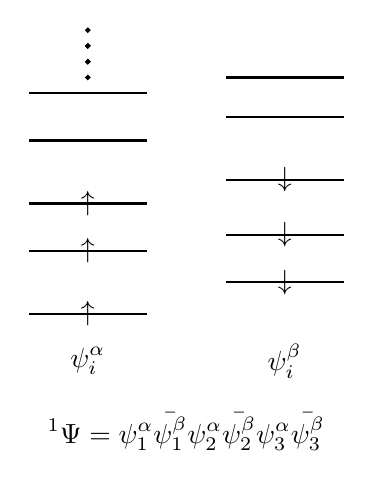
\begin{tikzpicture}[thick]
	\draw (2, -1.5)node{$\displaystyle {^1\Psi} = \ket{\psi_1^\alpha\bar{\psi_1^\beta}\psi_2^\alpha\bar{\psi_2^\beta}\psi_3^\alpha\bar{\psi_3^\beta}}$};
	%=========== figure left, from bottom to top===========================
	\draw (.75, -.6)node{$\displaystyle {\psi_i^\alpha}$};
	\draw (0,0)-- ++(.5,0)-- node{$\uparrow$} ++(.5,0)-- ++(.5,0);
	\draw (0,.8)--++(.5,0)-- node{$\uparrow$} ++(.5,0)node{}-- ++(.5,0);
	\draw (0,1.4)--++(.5,0)--node{$\uparrow$} ++(.5,0)node{}-- ++(.5,0);
	\draw (0,2.2)--++(.5,0)node{}-- ++(.5,0)node{}-- ++(.5,0);
	\draw (0,2.8)--++(.5,0)node{}-- ++(.5,0)node{}-- ++(.5,0);
	\filldraw (0.75,3)circle(.5pt) (.75,3.2)circle(.5pt) (.75,3.4)circle(.5pt);
	%=========== figure right, from bottom to top===========================
	\draw (3.25, -.6)node{$\displaystyle {\psi_i^\beta}$};
	\draw (2.5,.4)-- ++(.5,0)-- node{$\downarrow$} ++(.5,0)-- ++(.5,0);
	\draw (2.5,1)--++(.5,0)-- node{$\downarrow$} ++(.5,0)node{}-- ++(.5,0);
	\draw (2.5,1.7)--++(.5,0)--node{$\downarrow$} ++(.5,0)node{}-- ++(.5,0);
	\draw (2.5,2.5)--++(.5,0)node{}-- ++(.5,0)node{}-- ++(.5,0);
	\draw (2.5,3)--++(.5,0)node{}-- ++(.5,0)node{}-- ++(.5,0);
	\filldraw (0.75,3.2)circle(.5pt) (.75,3.4)circle(.5pt) (.75,3.6)circle(.5pt);
	\end{tikzpicture}
	\caption{一个\emph{近似}为单重态的非限制性行列式. }
        \label{fig:2.14}
\end{figure}
非限制性单态常会收敛到对应的限制性单态上, 
也就是闭壳层状态. 
举个例子, 
在我们的\phrase{极小基 $\hd$}中, 
在正常的键长下, 
闭壳层基态是$\ket{\psi_1\bar{\psi}_1}$, 
如果两个电子的空间部分不一样, 
那么能量会上升而非下降. 
但是当键长很大时, 
一个电子等效地处于一个氢核旁边, 
另一个电子处在另一个核旁边, 
那么这两个电子的空间部分应该很不相同. 
因此在大键长下, 
使用非限制性行列式要闭限制性所得的能量更低, 
正如我们在下一章将看到的那样.


若$N^\alpha=N^\beta+1$, 
那么非限制性行列式近似地为双重态(见\autoref{fig:2.15}). 
非限制性双重态常作为自由基的初级描述, 
自由基有一个未配对电子, 
如$\mathrm{CH}_3$. 
近似的三重态$\alpha$电子比$\beta$电子多两个, 
如\autoref{fig:2.16}所示.


若$\ket{1},\ket{2},\ket{3}$等是精确的自旋单、双、三…态, 
那么\autoref{fig:2.14},
\autoref{fig:2.15}, 
\autoref{fig:2.16}中的非限制性态可以展开为:
\begin{subequations}
	\begin{align}
	\ket{^1\Psi} = c_1^1\ket{1} + c_3^1\ket{3} + c_5^1\ket{5} + \cdots\\
	\ket{^2\Psi} = c_2^2\ket{2} + c_4^2\ket{4} + c_6^2\ket{6} + \cdots\\
	\ket{^3\Psi} = c_3^3\ket{3} + c_5^3\ket{5} + c_7^3\ket{7} + \cdots  
	\end{align}
\end{subequations}
可以看出非限制波函数会包含更高自旋多重度的态, 
而不包含更低的. 
如果以上展式中领头项占主导地位, 

\begin{figure}
	\begin{minipage}{.48\textwidth}
	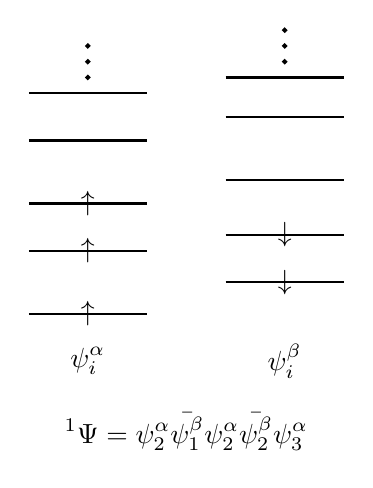
\begin{tikzpicture}[thick]
        \draw (2, -1.5)node{$\displaystyle {^1\Psi} = \ket{\psi_2^\alpha\bar{\psi_1^\beta}\psi_2^\alpha\bar{\psi_2^\beta}\psi_3^\alpha}$};
	%=========== figure left, from bottom to top===========================
	\draw (.75, -.6)node{$\displaystyle {\psi_i^\alpha}$};
	\draw (0,0)-- ++(.5,0)-- node{$\uparrow$} ++(.5,0)-- ++(.5,0);
	\draw (0,.8)--++(.5,0)-- node{$\uparrow$} ++(.5,0)node{}-- ++(.5,0);
	\draw (0,1.4)--++(.5,0)--node{$\uparrow$} ++(.5,0)node{}-- ++(.5,0);
	\draw (0,2.2)--++(.5,0)node{}-- ++(.5,0)node{}-- ++(.5,0);
	\draw (0,2.8)--++(.5,0)node{}-- ++(.5,0)node{}-- ++(.5,0);
	\filldraw (0.75,3)circle(.5pt) (.75,3.2)circle(.5pt) (.75,3.4)circle(.5pt);
	%=========== figure right, from bottom to top===========================
	\draw (3.25, -.6)node{$\displaystyle {\psi_i^\beta}$};
	\draw (2.5,.4)-- ++(.5,0)-- node{$\downarrow$} ++(.5,0)-- ++(.5,0);
	\draw (2.5,1)--++(.5,0)-- node{$\downarrow$} ++(.5,0)node{}-- ++(.5,0);
	\draw (2.5,1.7)--++(.5,0)--node{} ++(.5,0)node{}-- ++(.5,0);
	\draw (2.5,2.5)--++(.5,0)node{}-- ++(.5,0)node{}-- ++(.5,0);
	\draw (2.5,3)--++(.5,0)node{}-- ++(.5,0)node{}-- ++(.5,0);
	\filldraw (3.25,3.2)circle(.5pt) (3.25,3.4)circle(.5pt) (3.25,3.6)circle(.5pt);
	\end{tikzpicture}
	\caption{一个\emph{近似}为双重态的非限制性行列式. }
        \label{fig:2.15}
	\end{minipage}\qquad
	\begin{minipage}{.48\textwidth}
	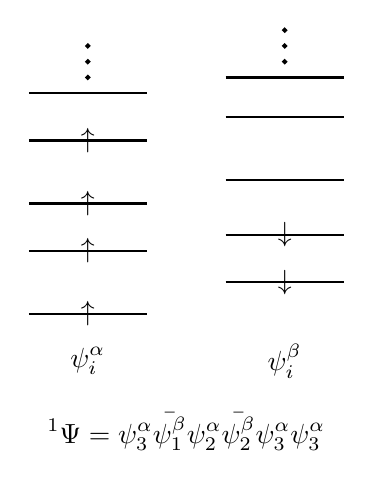
\begin{tikzpicture}[thick]
	\draw (2, -1.5)node{$\displaystyle {^1\Psi} = \ket{\psi_3^\alpha\bar{\psi_1^\beta}\psi_2^\alpha\bar{\psi_2^\beta}\psi_3^\alpha{\psi_3^\alpha}}$};
	%=========== figure left, from bottom to top===========================
	\draw (.75, -.6)node{$\displaystyle {\psi_i^\alpha}$};
	\draw (0,0)-- ++(.5,0)-- node{$\uparrow$} ++(.5,0)-- ++(.5,0);
	\draw (0,.8)--++(.5,0)-- node{$\uparrow$} ++(.5,0)node{}-- ++(.5,0);
	\draw (0,1.4)--++(.5,0)--node{$\uparrow$} ++(.5,0)node{}-- ++(.5,0);
	\draw (0,2.2)--++(.5,0)--node{$\uparrow$} ++(.5,0)node{}-- ++(.5,0);
	\draw (0,2.8)--++(.5,0)node{}-- ++(.5,0)node{}-- ++(.5,0);
	\filldraw (0.75,3)circle(.5pt) (.75,3.2)circle(.5pt) (.75,3.4)circle(.5pt);
	%=========== figure right, from bottom to top===========================
	\draw (3.25, -.6)node{$\displaystyle {\psi_i^\beta}$};
	\draw (2.5,.4)-- ++(.5,0)-- node{$\downarrow$} ++(.5,0)-- ++(.5,0);
	\draw (2.5,1)--++(.5,0)-- node{$\downarrow$} ++(.5,0)node{}-- ++(.5,0);
	\draw (2.5,1.7)--++(.5,0)--node{} ++(.5,0)node{}-- ++(.5,0);
	\draw (2.5,2.5)--++(.5,0)node{}-- ++(.5,0)node{}-- ++(.5,0);
	\draw (2.5,3)--++(.5,0)node{}-- ++(.5,0)node{}-- ++(.5,0);
	\filldraw (3.25,3.2)circle(.5pt) (3.25,3.4)circle(.5pt) (3.25,3.6)circle(.5pt);
	\end{tikzpicture}
	\caption{一个\emph{近似}为三重态的非限制性行列式. }
        \label{fig:2.16}
	\end{minipage}
\end{figure}
那么就可以将非限制性行列式近似作双重态、三重态等等. 
在非限制性行列式下, 
$\ts^2$的期望值常常过大, 
因为非自旋纯态(或称之为自旋污染态)的$S$值绘比纯态更大. 
具体而言, 
可以证明
\begin{align}\label{eq:2.271}
\braket{\ts^2}_\mathrm{UHF} = \braket{\ts^2}_\mathrm{Exact} + N^\beta - \sum_i^N\sum_j^N|S_{ij}^{\alpha\beta}|^2
\end{align}
式中已设$N^\alpha > N^\beta$, 
且
\begin{align}
	\braket{\ts^2}_\mathrm{Exact} = \left( \frac{N^\alpha - N^\beta}{2} \right) \left( \frac{N^\alpha - N^\beta}{2} + 1\right)
\end{align}
虽然有自旋污染这个问题, 
但非限制性行列式仍常用作双重态核三重态的第一次近似, 
因为非限制性行列式的能量比对应的限制性行列式更低.

 \exercise{
考虑行列式$\ket{K} = \ket{\psi_1^\alpha\bar{\psi}_1^\beta}$, 
它由\emph{非正交}的空间轨道构成:$\braket{\psi_1^\alpha|\psi_1^\beta} = S_{11}^{\alpha\beta}$. 
请证明只有当$\psi_1^\alpha=\psi_1^\beta$时$\ket{K}$才是$\ts^2$的本征函数. 
另外证明$\braket{K|\ts^2|K} = 1 - |S_{11}^{\alpha\beta}|^2$, 
与\autoref{eq:2.271}相吻合.

}

\theendnotes
\addcontentsline{toc}{section}{注释}
\section*{拓展阅读}
\addcontentsline{toc}{section}{拓展阅读}

\indent Avery, J., \textit{Creation and Annihilation Operators}, McGraw-Hill, New York, 1976. 
此书第二章用二次量子化的语言梳理了量子力学中的各种近似, 包括Hartree-Fock近似.

Flurry, R. L. Jr., \textit{Symmetry Groups}, Prentice Hall, Englewood Cliffs, New Jersey, 1980. 
这是一个对群论在化学中的应用的相当精彩的介绍. 您正在看的这本书假设您对基本的群论与相关的记号较为熟悉.

Mattuck, R. D., 2nd ed., \textit{A Guide to Feynman Diagrams in the Many-Body Problem}, McGraw-Hill, New York, 1976. 
第七章用比本书更高级的方式介绍了二次量子化.

McWeeny, R. and Sutcliffe, B. T., \textit{Methods of Molecular Quantum Mechanics}, 2nd ed., Academic Press, New York, 1976. 
讨论了计算由非正交自旋轨道构成的Slater行列式的矩阵元的规则. 该书也简明介绍了如何得到自旋本征函数.

Slater, J. C., \textit{Quantum Theory of Matter}, 2nd ed., McGraw-Hill, New York, 1968. 
第十一章讨论了行列式波函数, 并用略不同于本书的方式推导了行列式间的矩阵元.
